% resultados_lstm.tex  --  Sección 4.3
% Predicción LSTM para Cemento y Ladrillo Común

\section{Predicción de los Precios del Cemento y del Ladrillo Común con Long Short-Term Memory (LSTM)}

\vspace{0.3cm}
\justify
En esta sección se presentan los resultados de aplicar una red LSTM (\textit{Long Short-Term Memory}) a la predicción de los precios mensuales del cemento y del ladrillo común. Para cada material se entrenaron dos modelos independientes: uno para el escenario sin efecto pandémico y otro para el escenario con efecto pandémico. Ambos fueron implementados con TensorFlow 2.19.0 / Keras, y sus hiperparámetros fueron optimizados de forma independiente con Optuna. La partición temporal es idéntica en todos los casos: 95 meses de entrenamiento, 20 meses de validación y 22 meses de prueba. Las variables de entrada son 7: precio promedio polinomial de grado 2, nivel del río Paraguay, indicador de cuarentena COVID-19, rezago de un mes, media móvil de 3 meses, y las componentes sinusoidal y cosenoidal del mes. Los intervalos de confianza al 95\,\% se estimaron mediante Monte Carlo Dropout ($N=100$ simulaciones).

% ============================================================
%  CEMENTO
% ============================================================
\subsection{Predicción del Precio del Cemento}

\justify
Para el cemento, la búsqueda de hiperparámetros con Optuna convergió a la misma configuración en ambos escenarios (sin y con efecto pandémico), lo que indica que la arquitectura óptima para esta serie es robusta a la inclusión o exclusión de la variable pandémica en el entrenamiento. Las métricas de evaluación sobre el conjunto de prueba son asimismo idénticas entre escenarios (RMSE de prueba: Gs.~1.619,75). Por esta razón, la descripción del modelo, la evaluación y el análisis de residuos se presentan una sola vez; los resultados se diferencian únicamente en el pronóstico a 24 meses.

\subsubsection{Análisis Exploratorio de la Serie}

\begin{figure}[htbp]
    \centering
    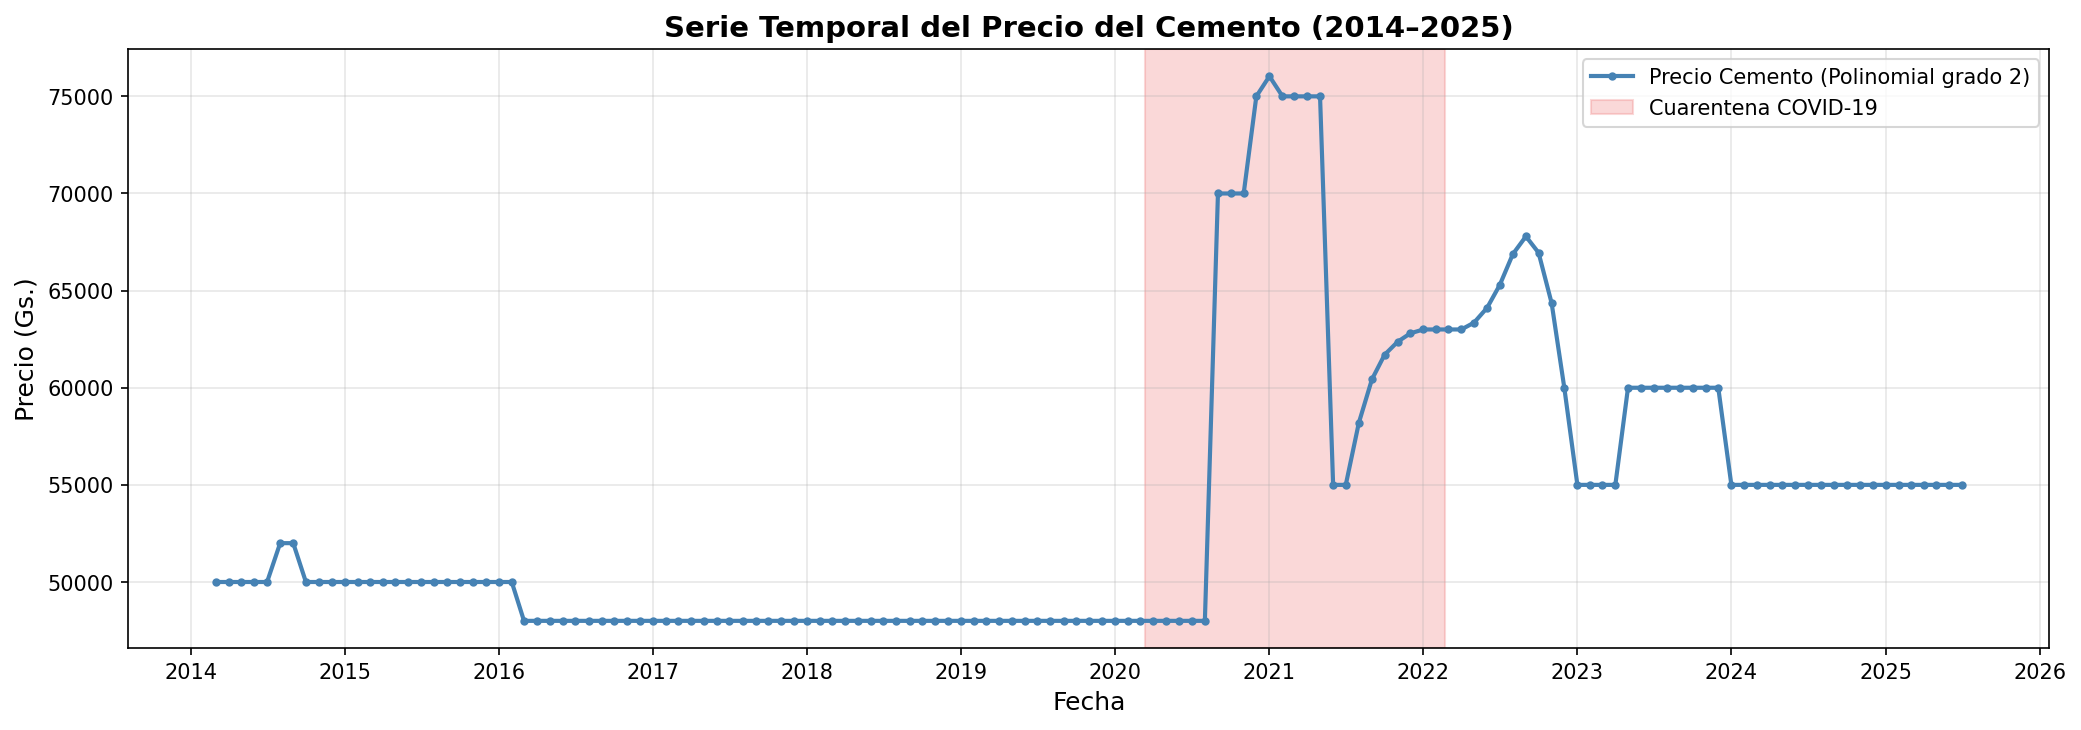
\includegraphics[width=\textwidth]{predicciones/prediccion_cemento_lstm/resultados_sin_covid/eda_01_serie_precios_cemento.png}
    \caption{Serie histórica mensual del precio del cemento (Gs.), período 2014--2025.}
    \label{fig:lstm_cemento_eda_serie}
\end{figure}

\begin{figure}[htbp]
    \centering
    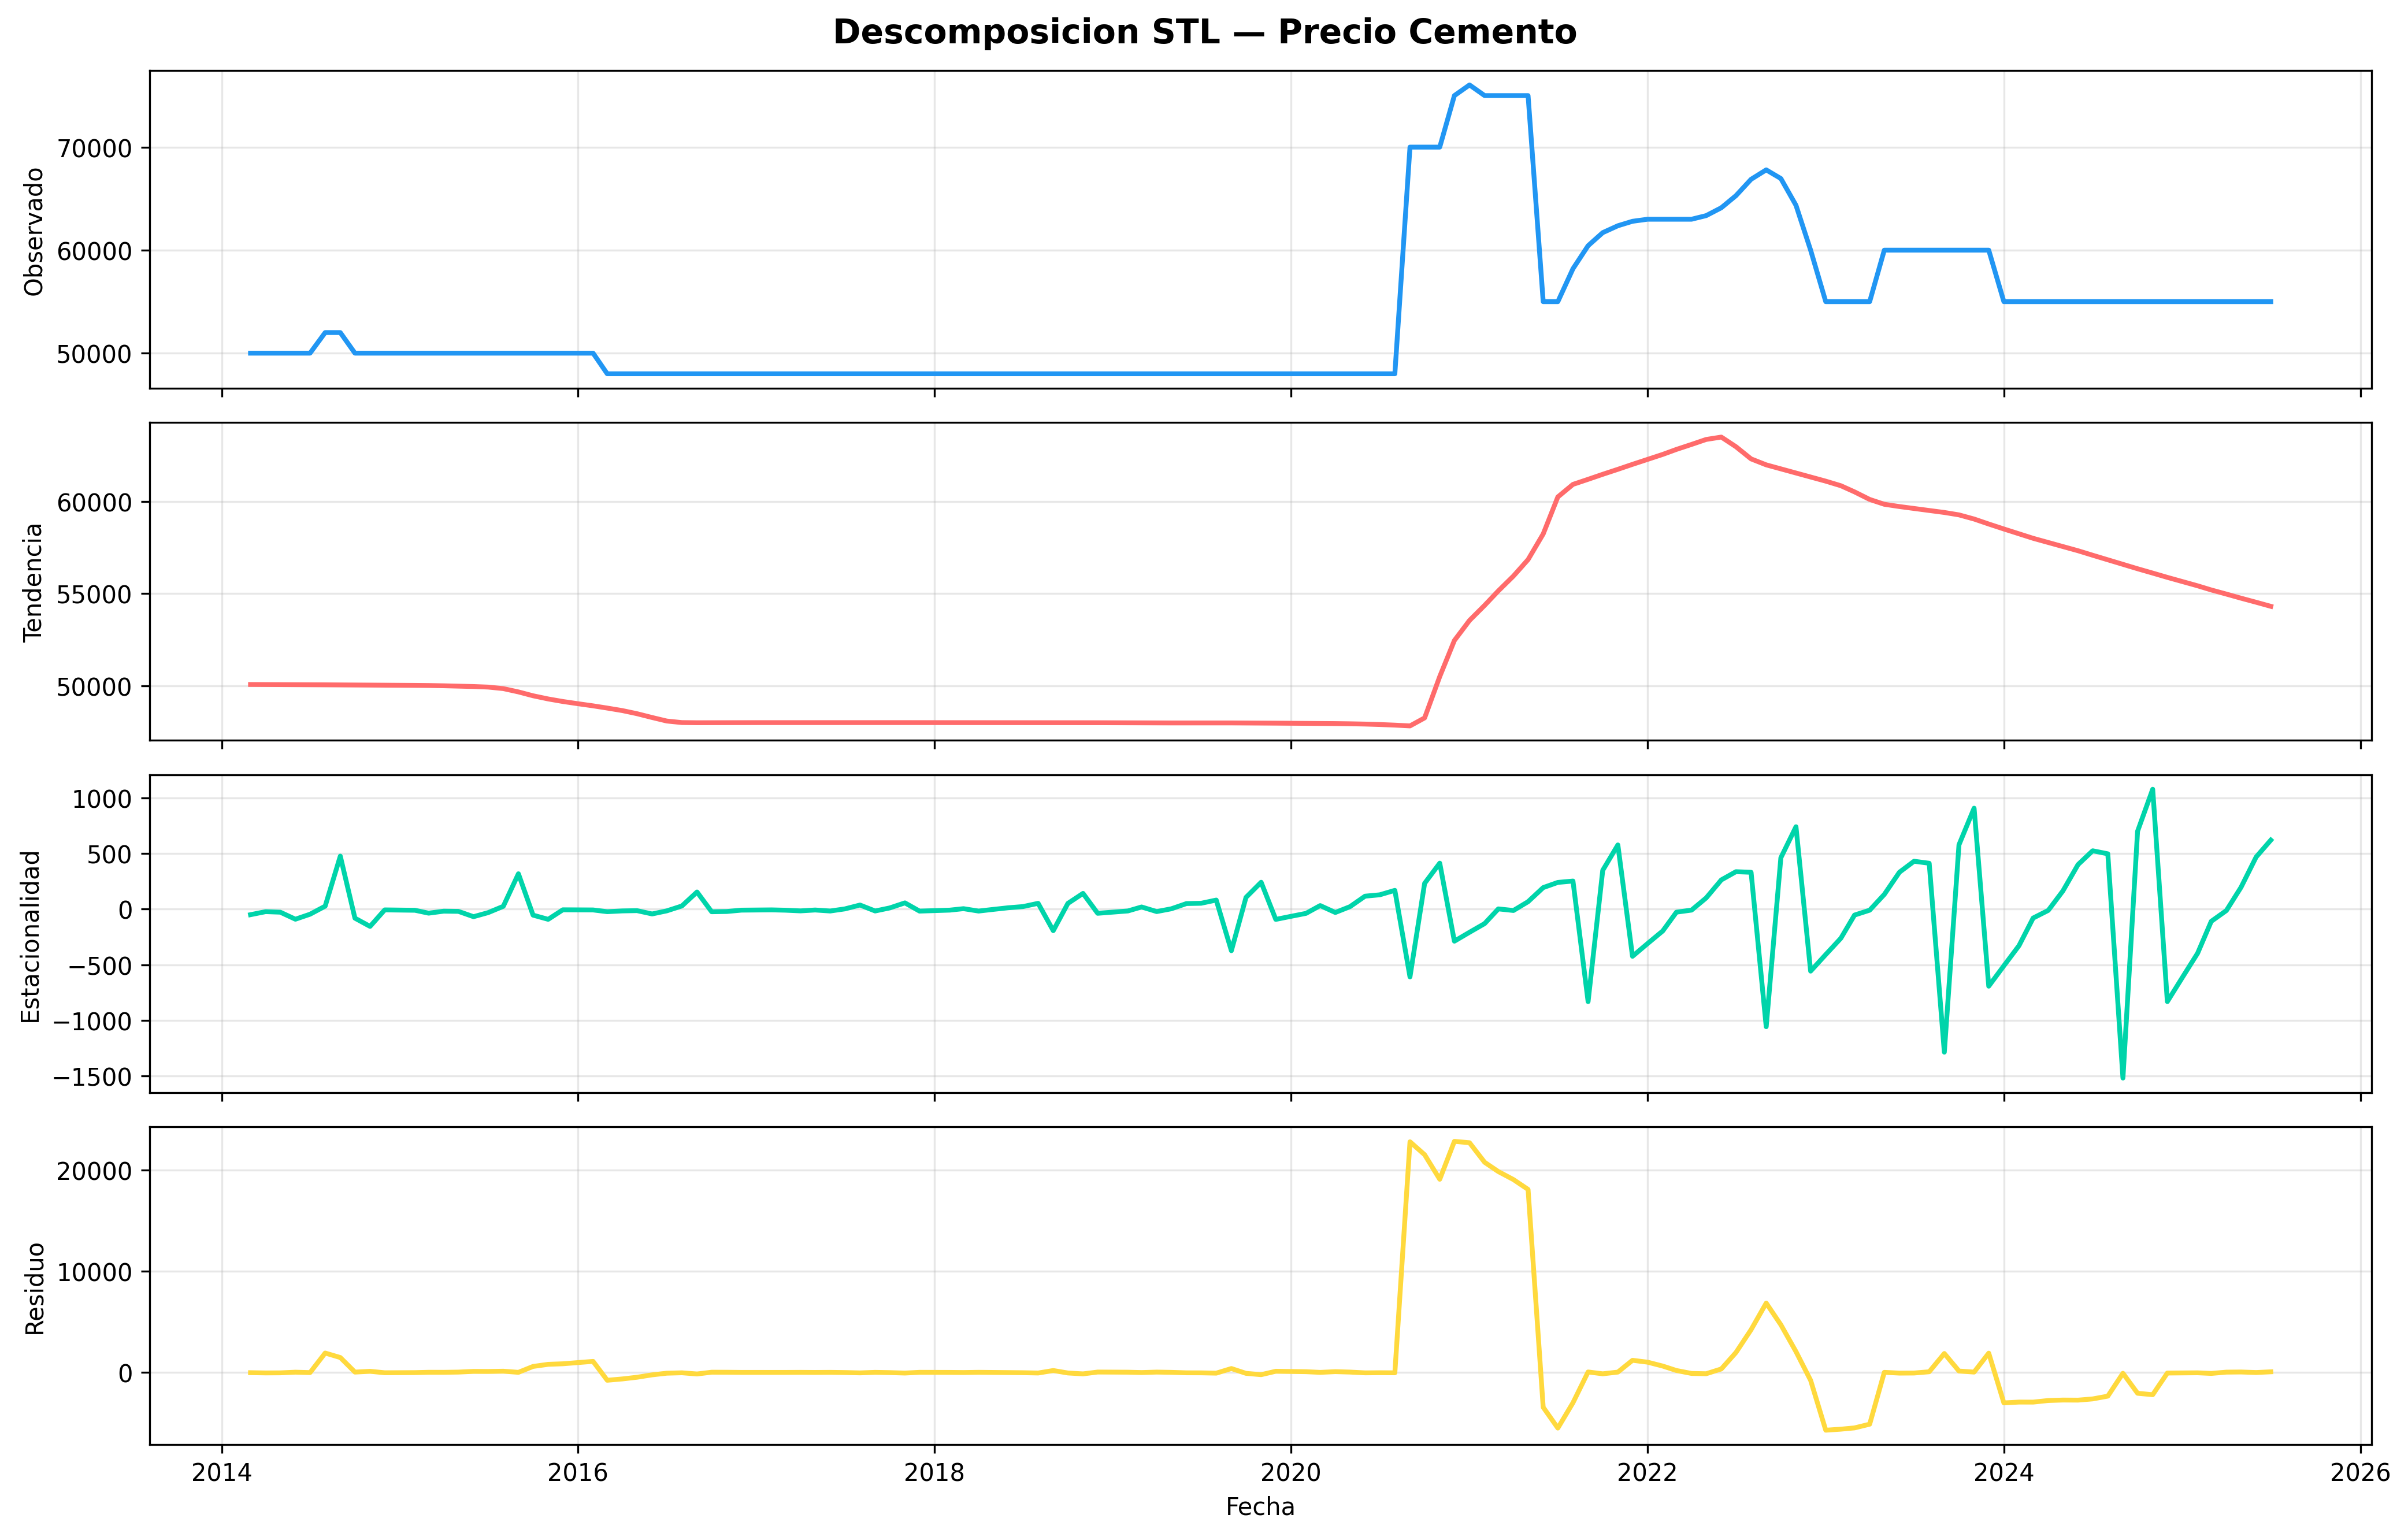
\includegraphics[width=\textwidth]{predicciones/prediccion_cemento_lstm/resultados_sin_covid/eda_stl_decomposition.png}
    \caption{Descomposición STL de la serie del precio del cemento: tendencia, estacionalidad y residuo.}
    \label{fig:lstm_cemento_eda_stl}
\end{figure}

\begin{figure}[htbp]
    \centering
    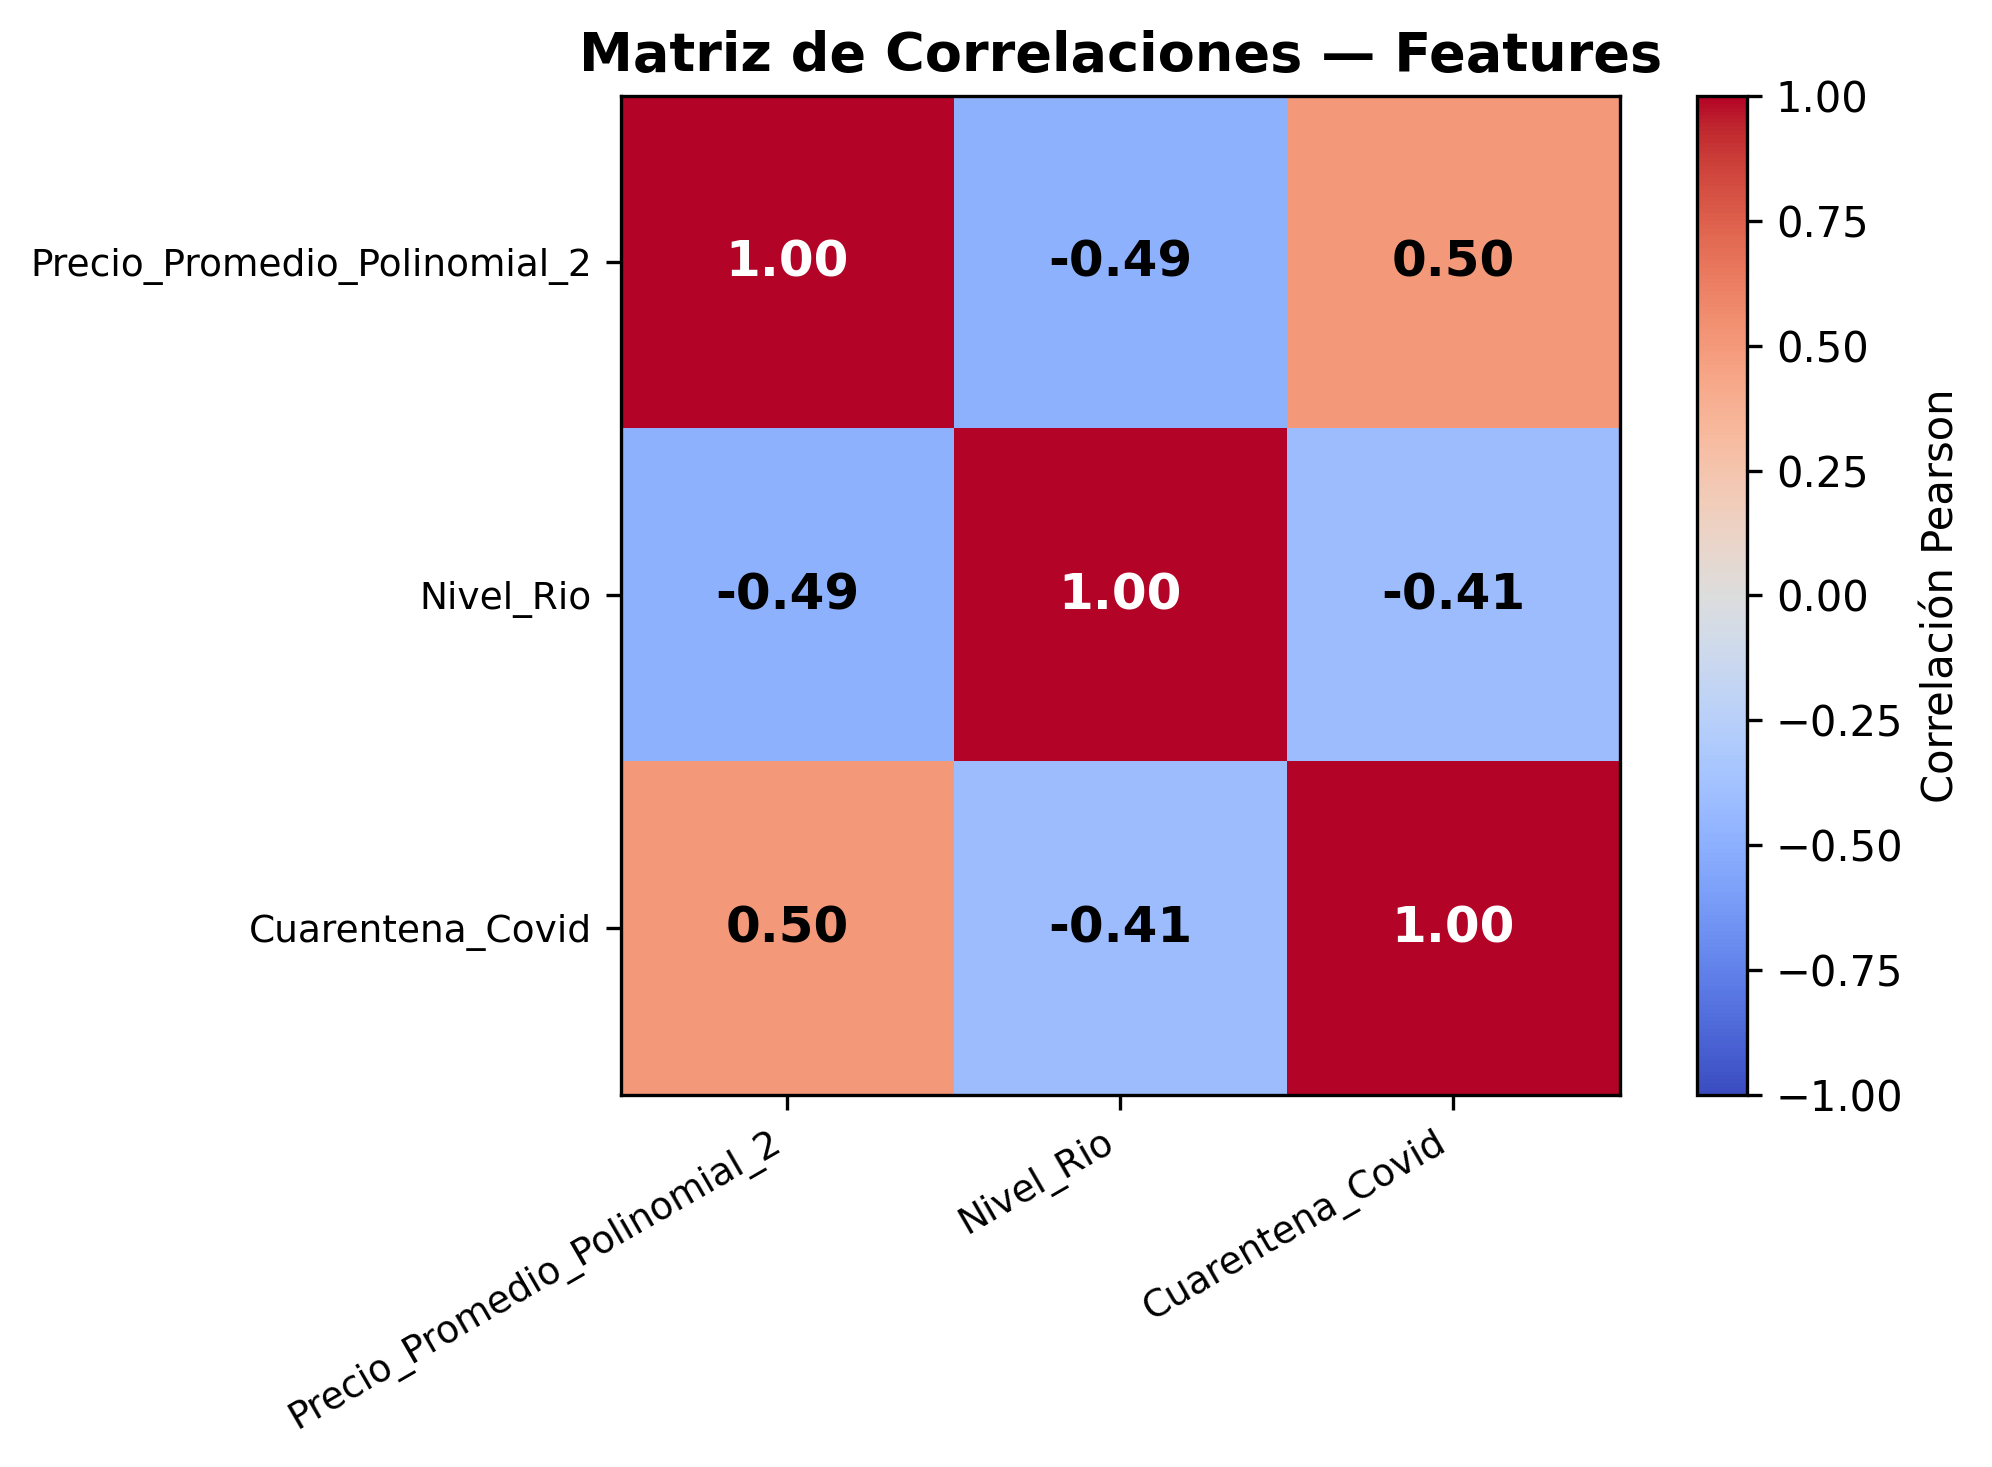
\includegraphics[width=\textwidth]{predicciones/prediccion_cemento_lstm/resultados_sin_covid/eda_correlaciones_heatmap.png}
    \caption{Mapa de calor de correlaciones entre las variables de entrada del modelo LSTM para cemento.}
    \label{fig:lstm_cemento_eda_corr}
\end{figure}

\subsubsection{Hiperparámetros y Arquitectura}

\justify
La búsqueda automática de hiperparámetros con Optuna seleccionó una arquitectura de una sola capa LSTM con 64 unidades ocultas, sin bidireccionalidad ni \textit{dropout}. El optimizador elegido fue Adam con tasa de aprendizaje $\text{lr}=0{,}001$ y regularización de pesos $\lambda=10^{-5}$. El \textit{lookback} quedó fijado en 6 meses y el \textit{batch size} en 4. No se aplicó ningún \textit{scheduler} de tasa de aprendizaje. La Tabla~\ref{tab:lstm_cemento_hiper} resume estos parámetros.

\begin{table}[htbp]
\centering
\caption{Hiperparámetros óptimos del modelo LSTM para cemento, seleccionados por Optuna.}
\label{tab:lstm_cemento_hiper}
\begin{tabular}{ll}
\toprule
\textbf{Hiperparámetro} & \textbf{Valor} \\
\midrule
Capas LSTM          & 1 \\
Unidades ocultas    & 64 \\
Bidireccional       & No \\
Dropout             & 0,0 \\
Dropout recurrente  & 0,0 \\
Optimizador         & Adam \\
Tasa de aprendizaje & 0,001 \\
Regularización L2   & $10^{-5}$ \\
Lookback            & 6 meses \\
Batch size          & 4 \\
Scheduler           & Ninguno \\
Parámetros entrenables & 18.497 \\
\bottomrule
\end{tabular}
\end{table}

\subsubsection{Curva de Aprendizaje}

\justify
El modelo final se entrenó durante 65 épocas sobre el conjunto de entrenamiento con \textit{early stopping} basado en el RMSE de validación. La Figura~\ref{fig:lstm_cemento_curva} muestra la evolución del error en ambas particiones.

\begin{figure}[htbp]
    \centering
    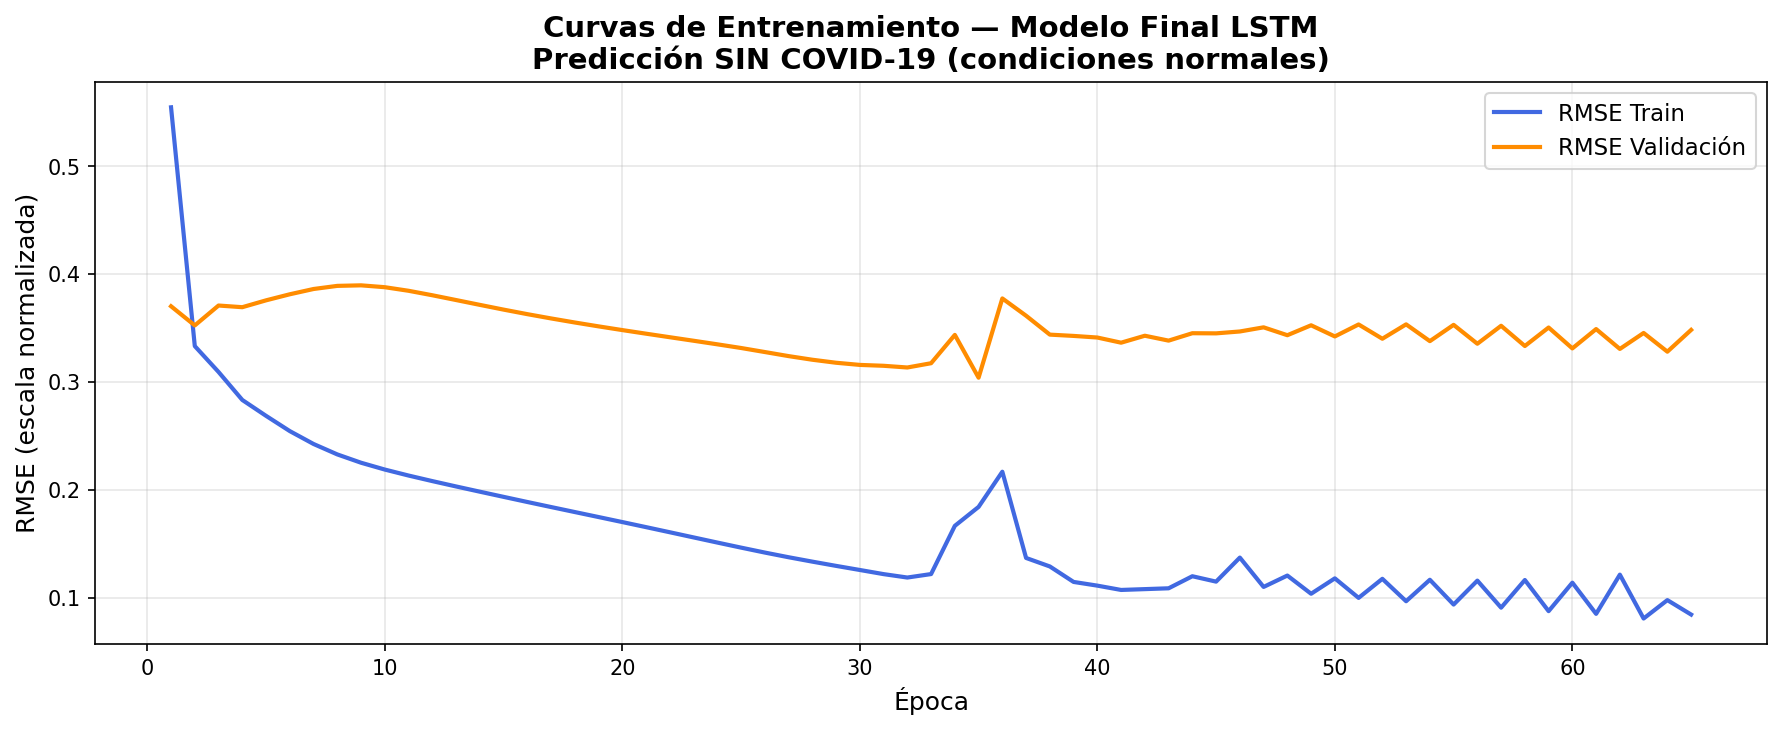
\includegraphics[width=0.85\textwidth]{predicciones/prediccion_cemento_lstm/resultados_sin_covid/final_01_curvas_entrenamiento.png}
    \caption{Curva de aprendizaje del modelo LSTM para cemento: RMSE de entrenamiento y validación por época.}
    \label{fig:lstm_cemento_curva}
\end{figure}

\justify
Se observa que el error de entrenamiento desciende rápidamente durante las primeras épocas y se estabiliza, mientras que el error de validación converge hacia un nivel ligeramente superior sin divergir de manera sostenida. Este comportamiento indica que el modelo generaliza correctamente sin presentar sobreajuste severo.

\subsubsection{Métricas de Evaluación}

\justify
La Tabla~\ref{tab:lstm_cemento_metricas} presenta el RMSE obtenido en los tres subconjuntos de datos, expresado en Guaraníes (Gs.).

\begin{table}[htbp]
\centering
\caption{Desempeño del modelo LSTM para cemento: RMSE en entrenamiento, validación y prueba.}
\label{tab:lstm_cemento_metricas}
\begin{tabular}{lrrr}
\toprule
\textbf{Métrica} & \textbf{Train} & \textbf{Val} & \textbf{Test} \\
\midrule
RMSE (Gs.) & 1.828,74 & 4.261,22 & 1.619,75 \\
\bottomrule
\end{tabular}
\end{table}

\justify
El RMSE de prueba de 1.619,75~Gs.\ resulta inferior al de entrenamiento (1.828,74~Gs.), lo que indica que el modelo no ha memorizado los datos de entrenamiento. El error de validación más elevado (4.261,22~Gs.) refleja que ese subconjunto contiene meses con mayor volatilidad de precios. En términos relativos, considerando que el precio del cemento oscila históricamente en el rango de Gs.~48.000 a Gs.~76.036, el RMSE de prueba representa un error relativo inferior al 4\%, resultado aceptable para una predicción mensual a nivel de mercado.

\subsubsection{Evaluación sobre el Conjunto de Prueba}

\begin{figure}[htbp]
    \centering
    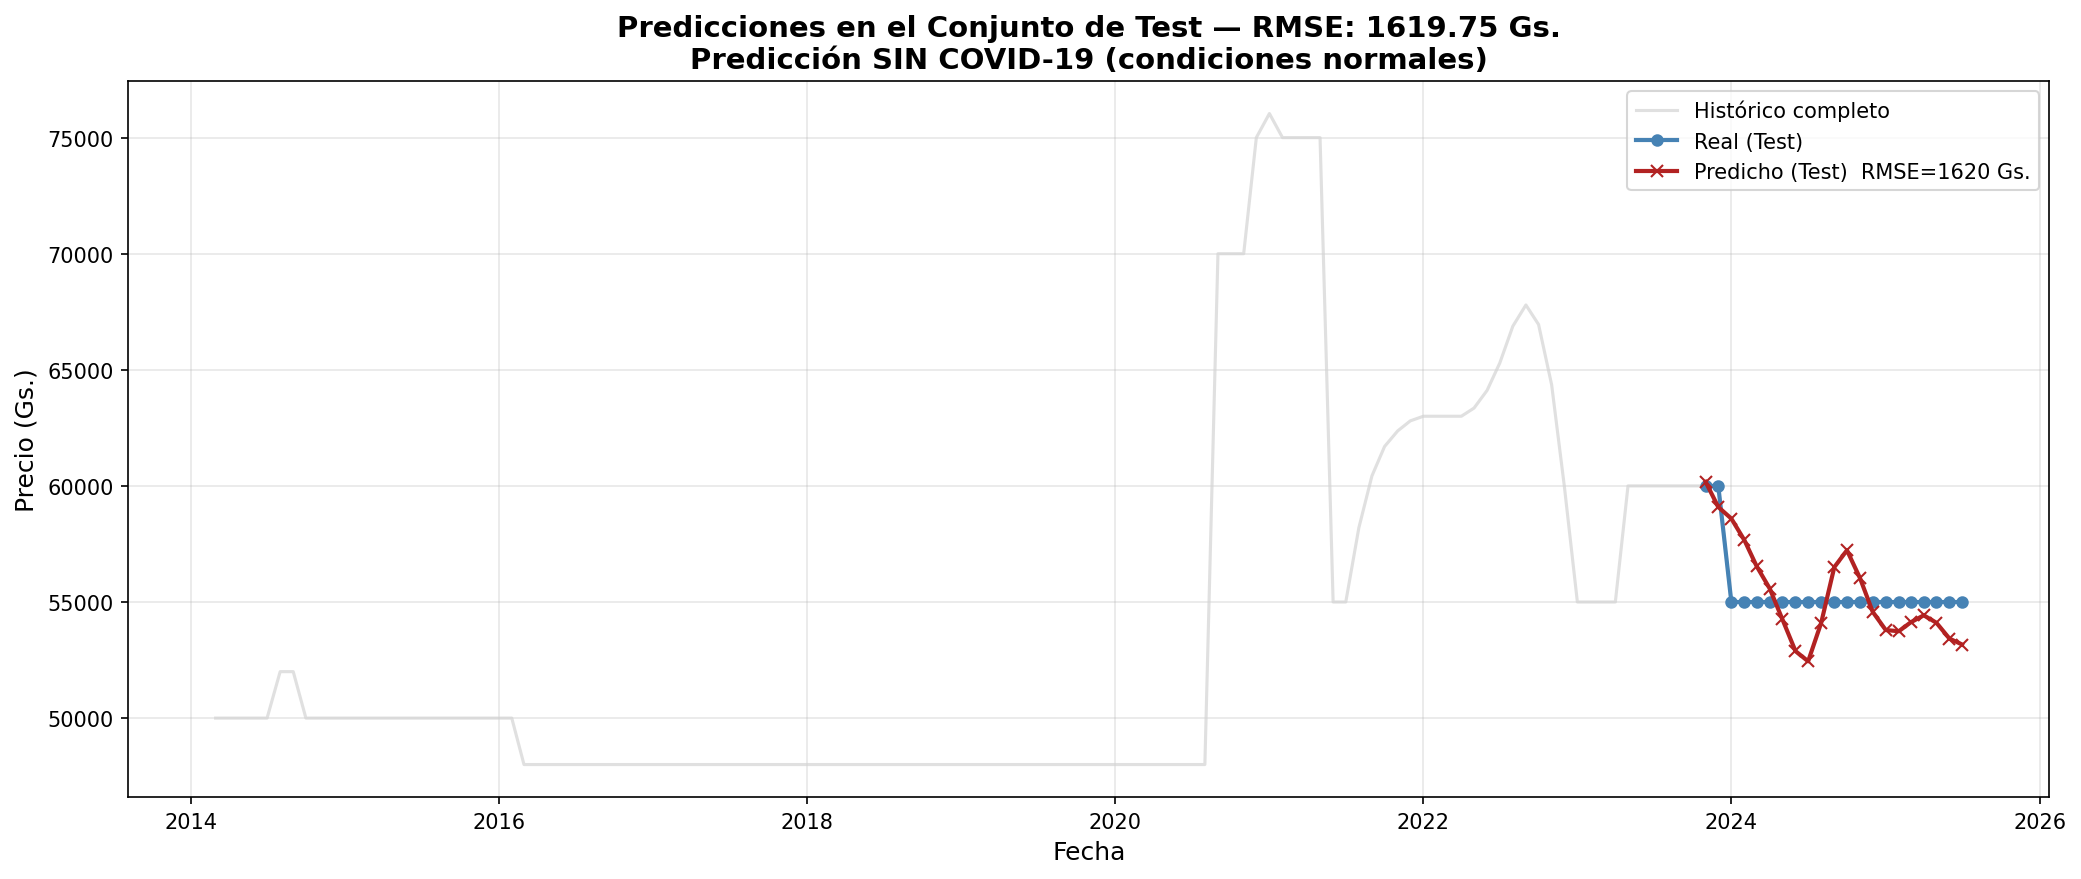
\includegraphics[width=\textwidth]{predicciones/prediccion_cemento_lstm/resultados_sin_covid/final_02_prediccion_test_serie.png}
    \caption{Predicción del modelo LSTM vs.\ valores reales del precio del cemento en el conjunto de prueba (22 meses).}
    \label{fig:lstm_cemento_test_serie}
\end{figure}

\begin{figure}[htbp]
    \centering
    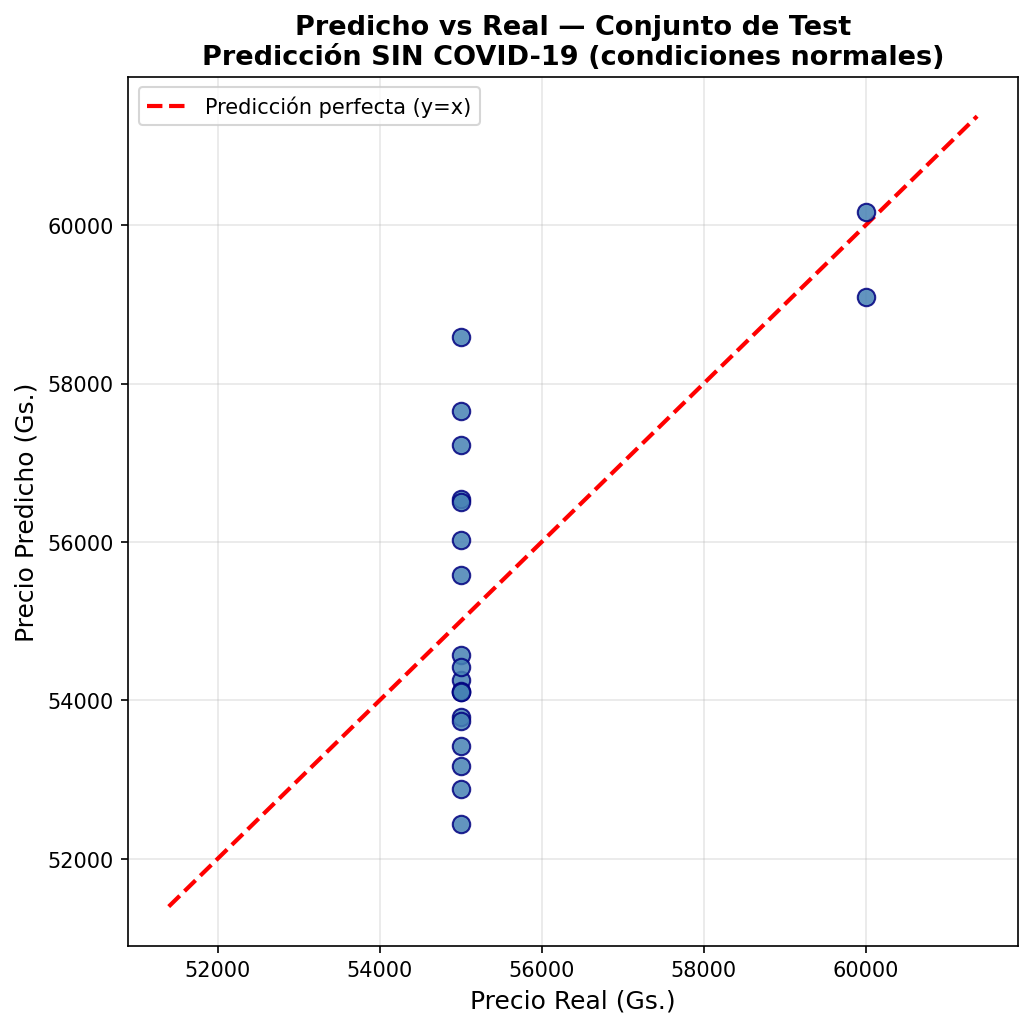
\includegraphics[width=0.7\textwidth]{predicciones/prediccion_cemento_lstm/resultados_sin_covid/final_03_scatter_test.png}
    \caption{Diagrama de dispersión: precio predicho vs.\ precio real del cemento en el conjunto de prueba.}
    \label{fig:lstm_cemento_scatter}
\end{figure}

\begin{figure}[htbp]
    \centering
    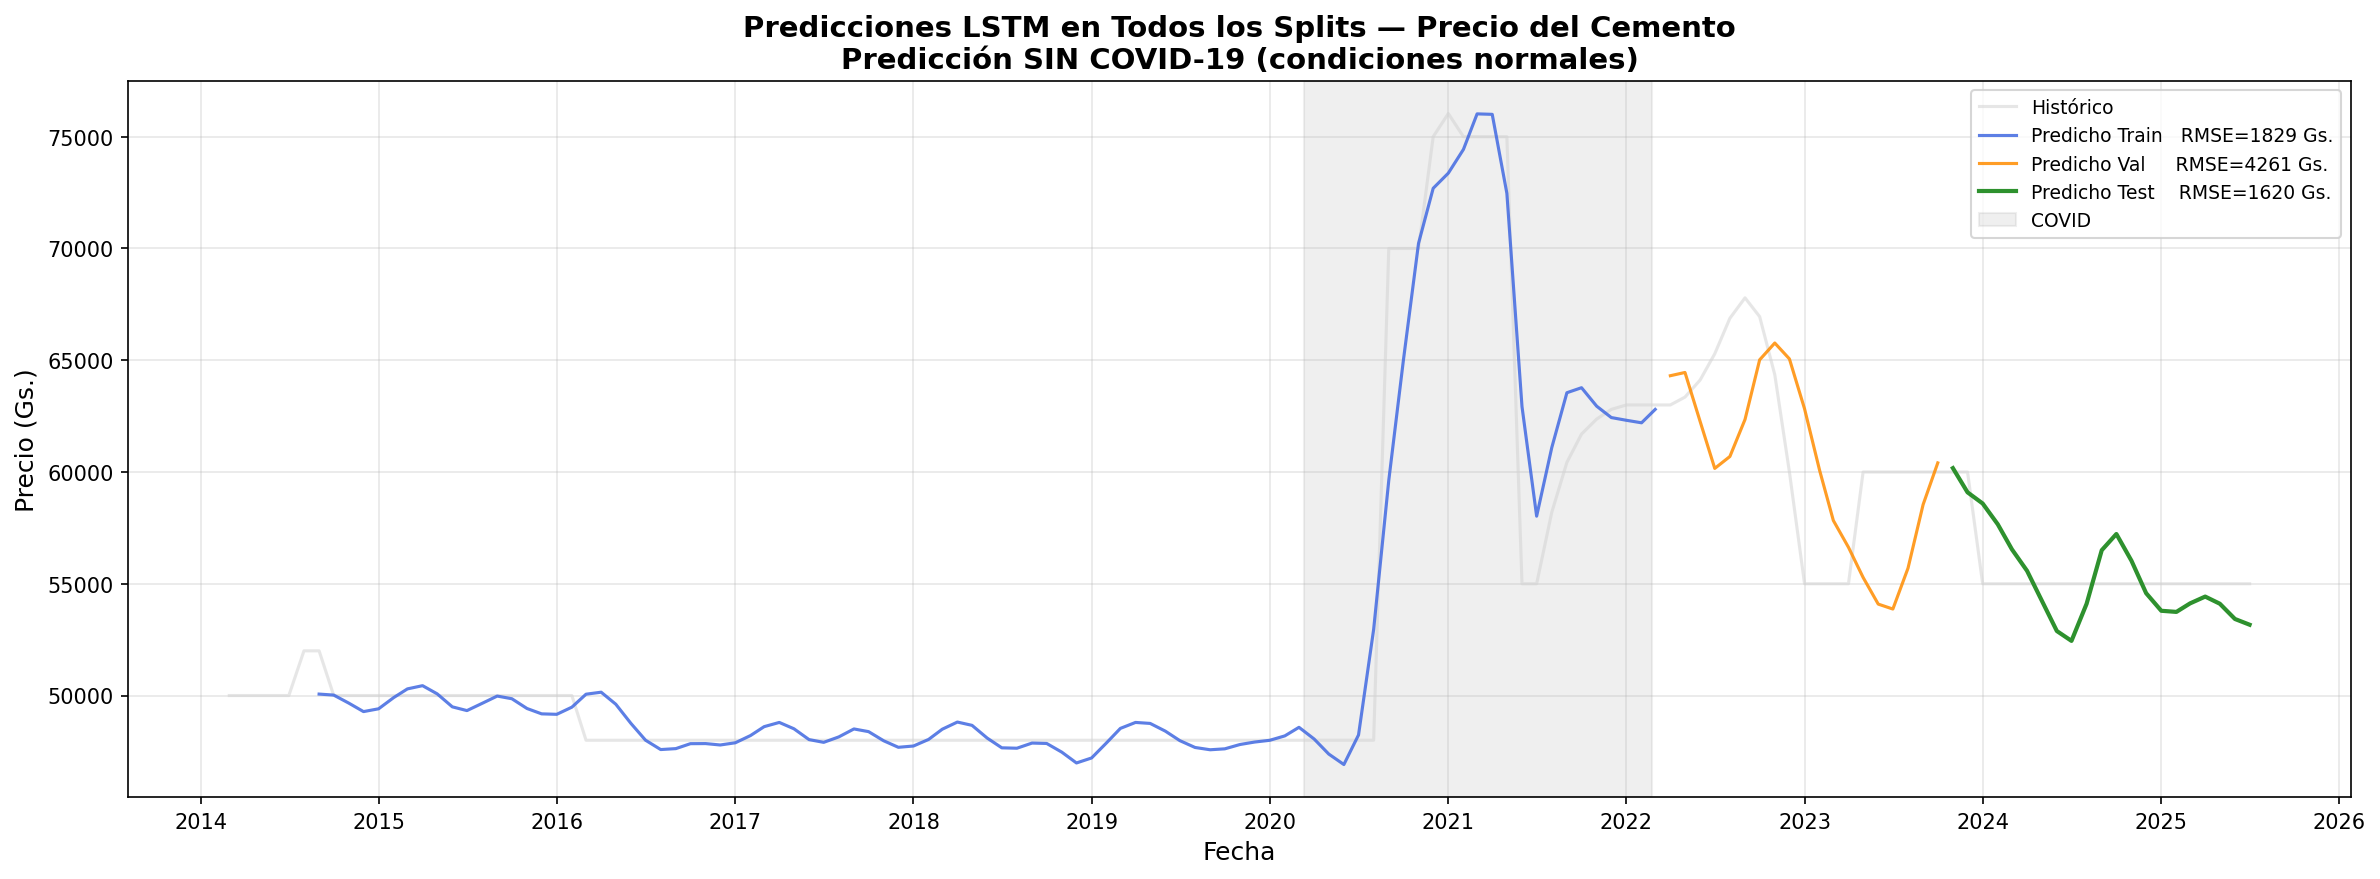
\includegraphics[width=\textwidth]{predicciones/prediccion_cemento_lstm/resultados_sin_covid/final_05_todos_splits.png}
    \caption{Predicción del modelo LSTM para cemento sobre los tres subconjuntos: entrenamiento, validación y prueba.}
    \label{fig:lstm_cemento_splits}
\end{figure}

\justify
La Figura~\ref{fig:lstm_cemento_test_serie} muestra la comparación entre los valores reales y predichos sobre el conjunto de prueba. El modelo captura la tendencia general de los precios siguiendo razonablemente bien las fluctuaciones observadas. Los puntos en el diagrama de dispersión (Figura~\ref{fig:lstm_cemento_scatter}) se agrupan en torno a la diagonal de 45°, confirmando la concordancia entre predichos y reales.

\clearpage
\subsubsection{Análisis de Residuos}

\begin{figure}[htbp]
    \centering
    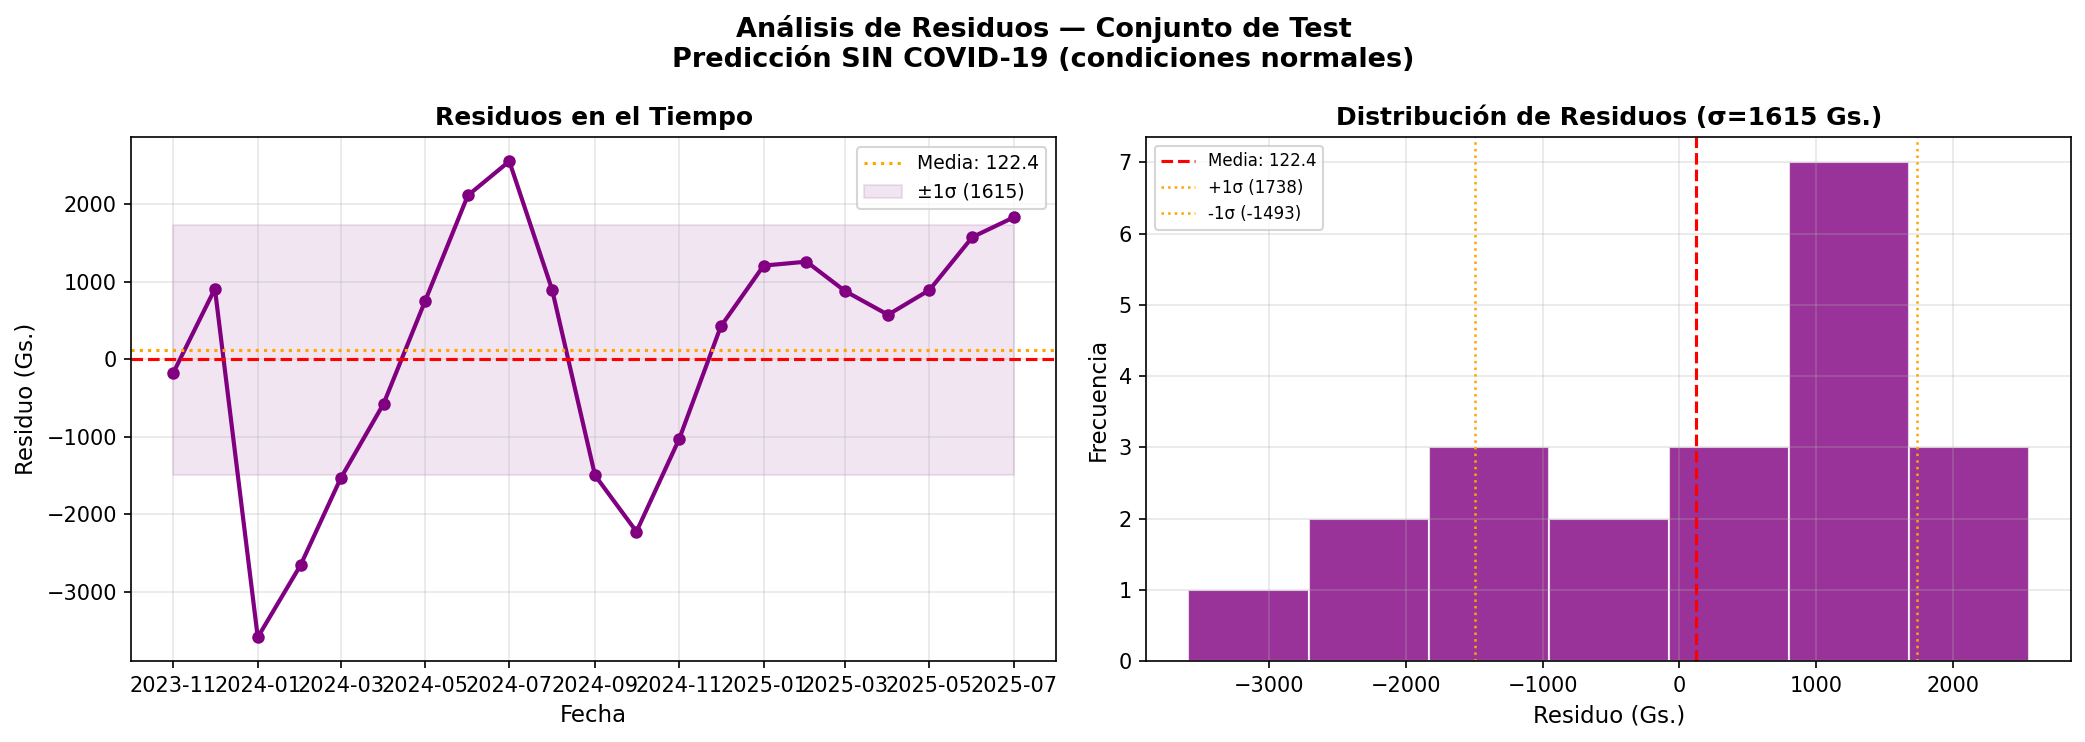
\includegraphics[width=\textwidth]{predicciones/prediccion_cemento_lstm/resultados_sin_covid/final_04_residuos.png}
    \caption{Serie temporal de residuos del modelo LSTM para cemento sobre el conjunto de prueba.}
    \label{fig:lstm_cemento_residuos}
\end{figure}

\begin{figure}[htbp]
    \centering
    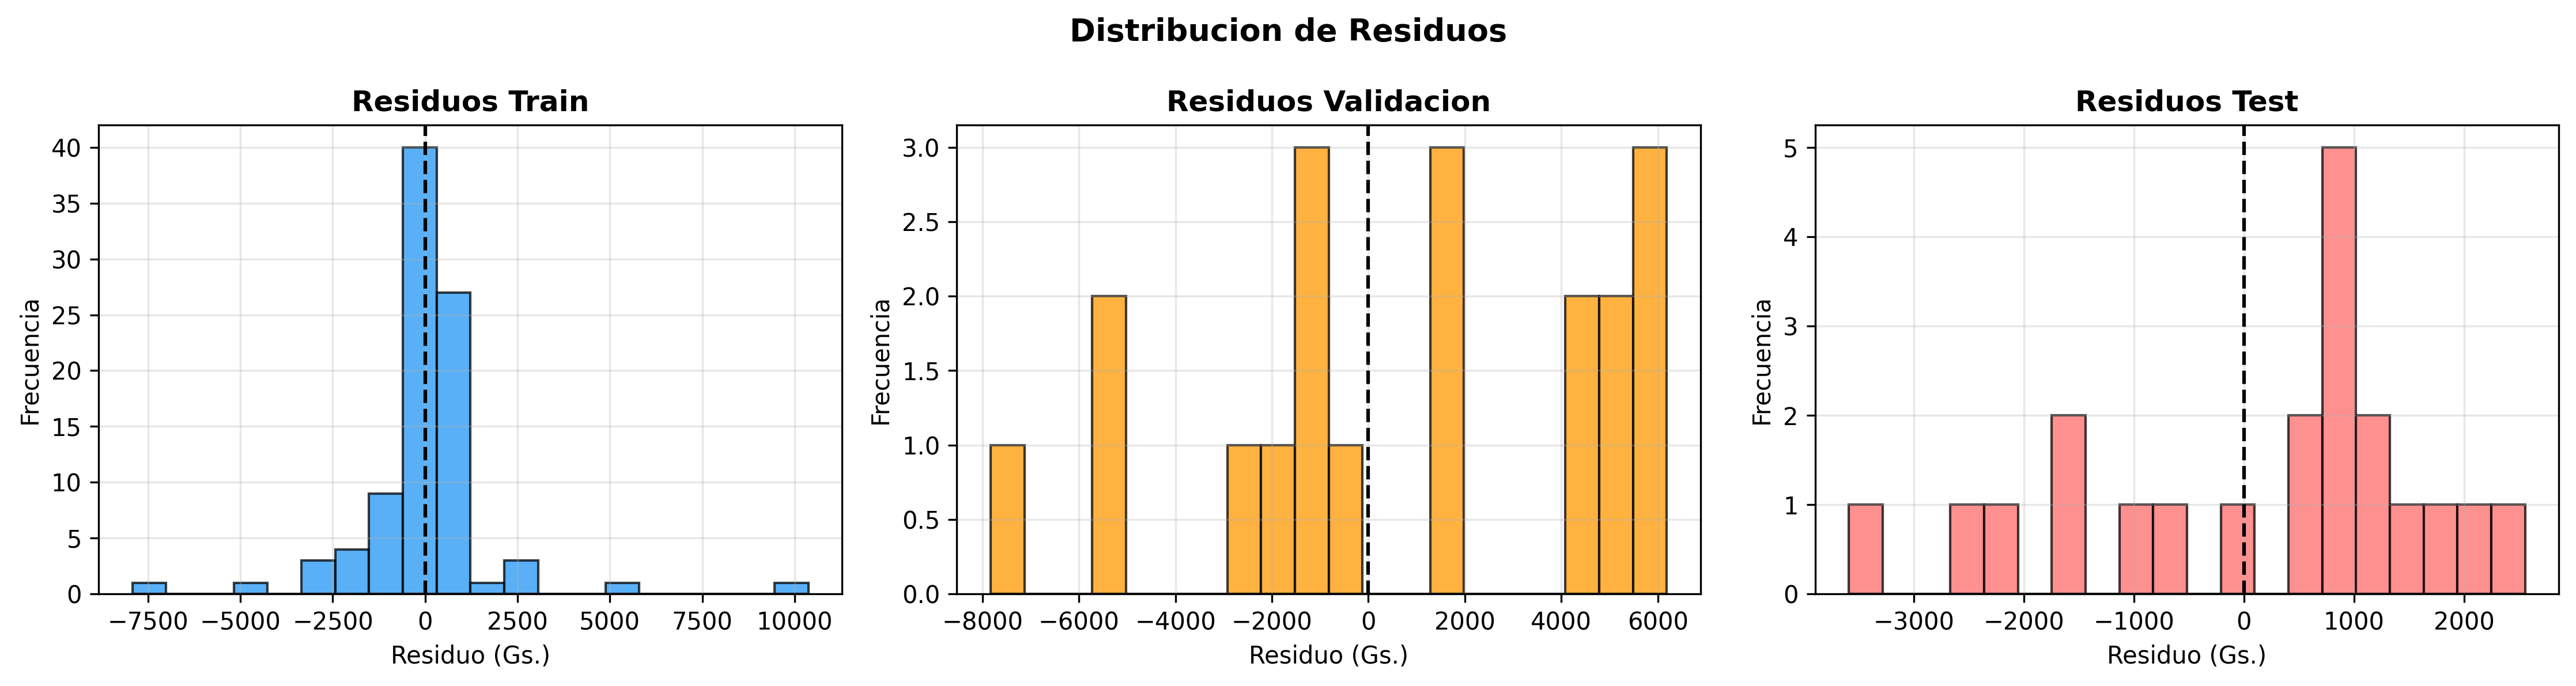
\includegraphics[width=0.75\textwidth]{predicciones/prediccion_cemento_lstm/resultados_sin_covid/residuos_histograma.png}
    \caption{Histograma de residuos del modelo LSTM para cemento.}
    \label{fig:lstm_cemento_residuos_hist}
\end{figure}

\begin{figure}[htbp]
    \centering
    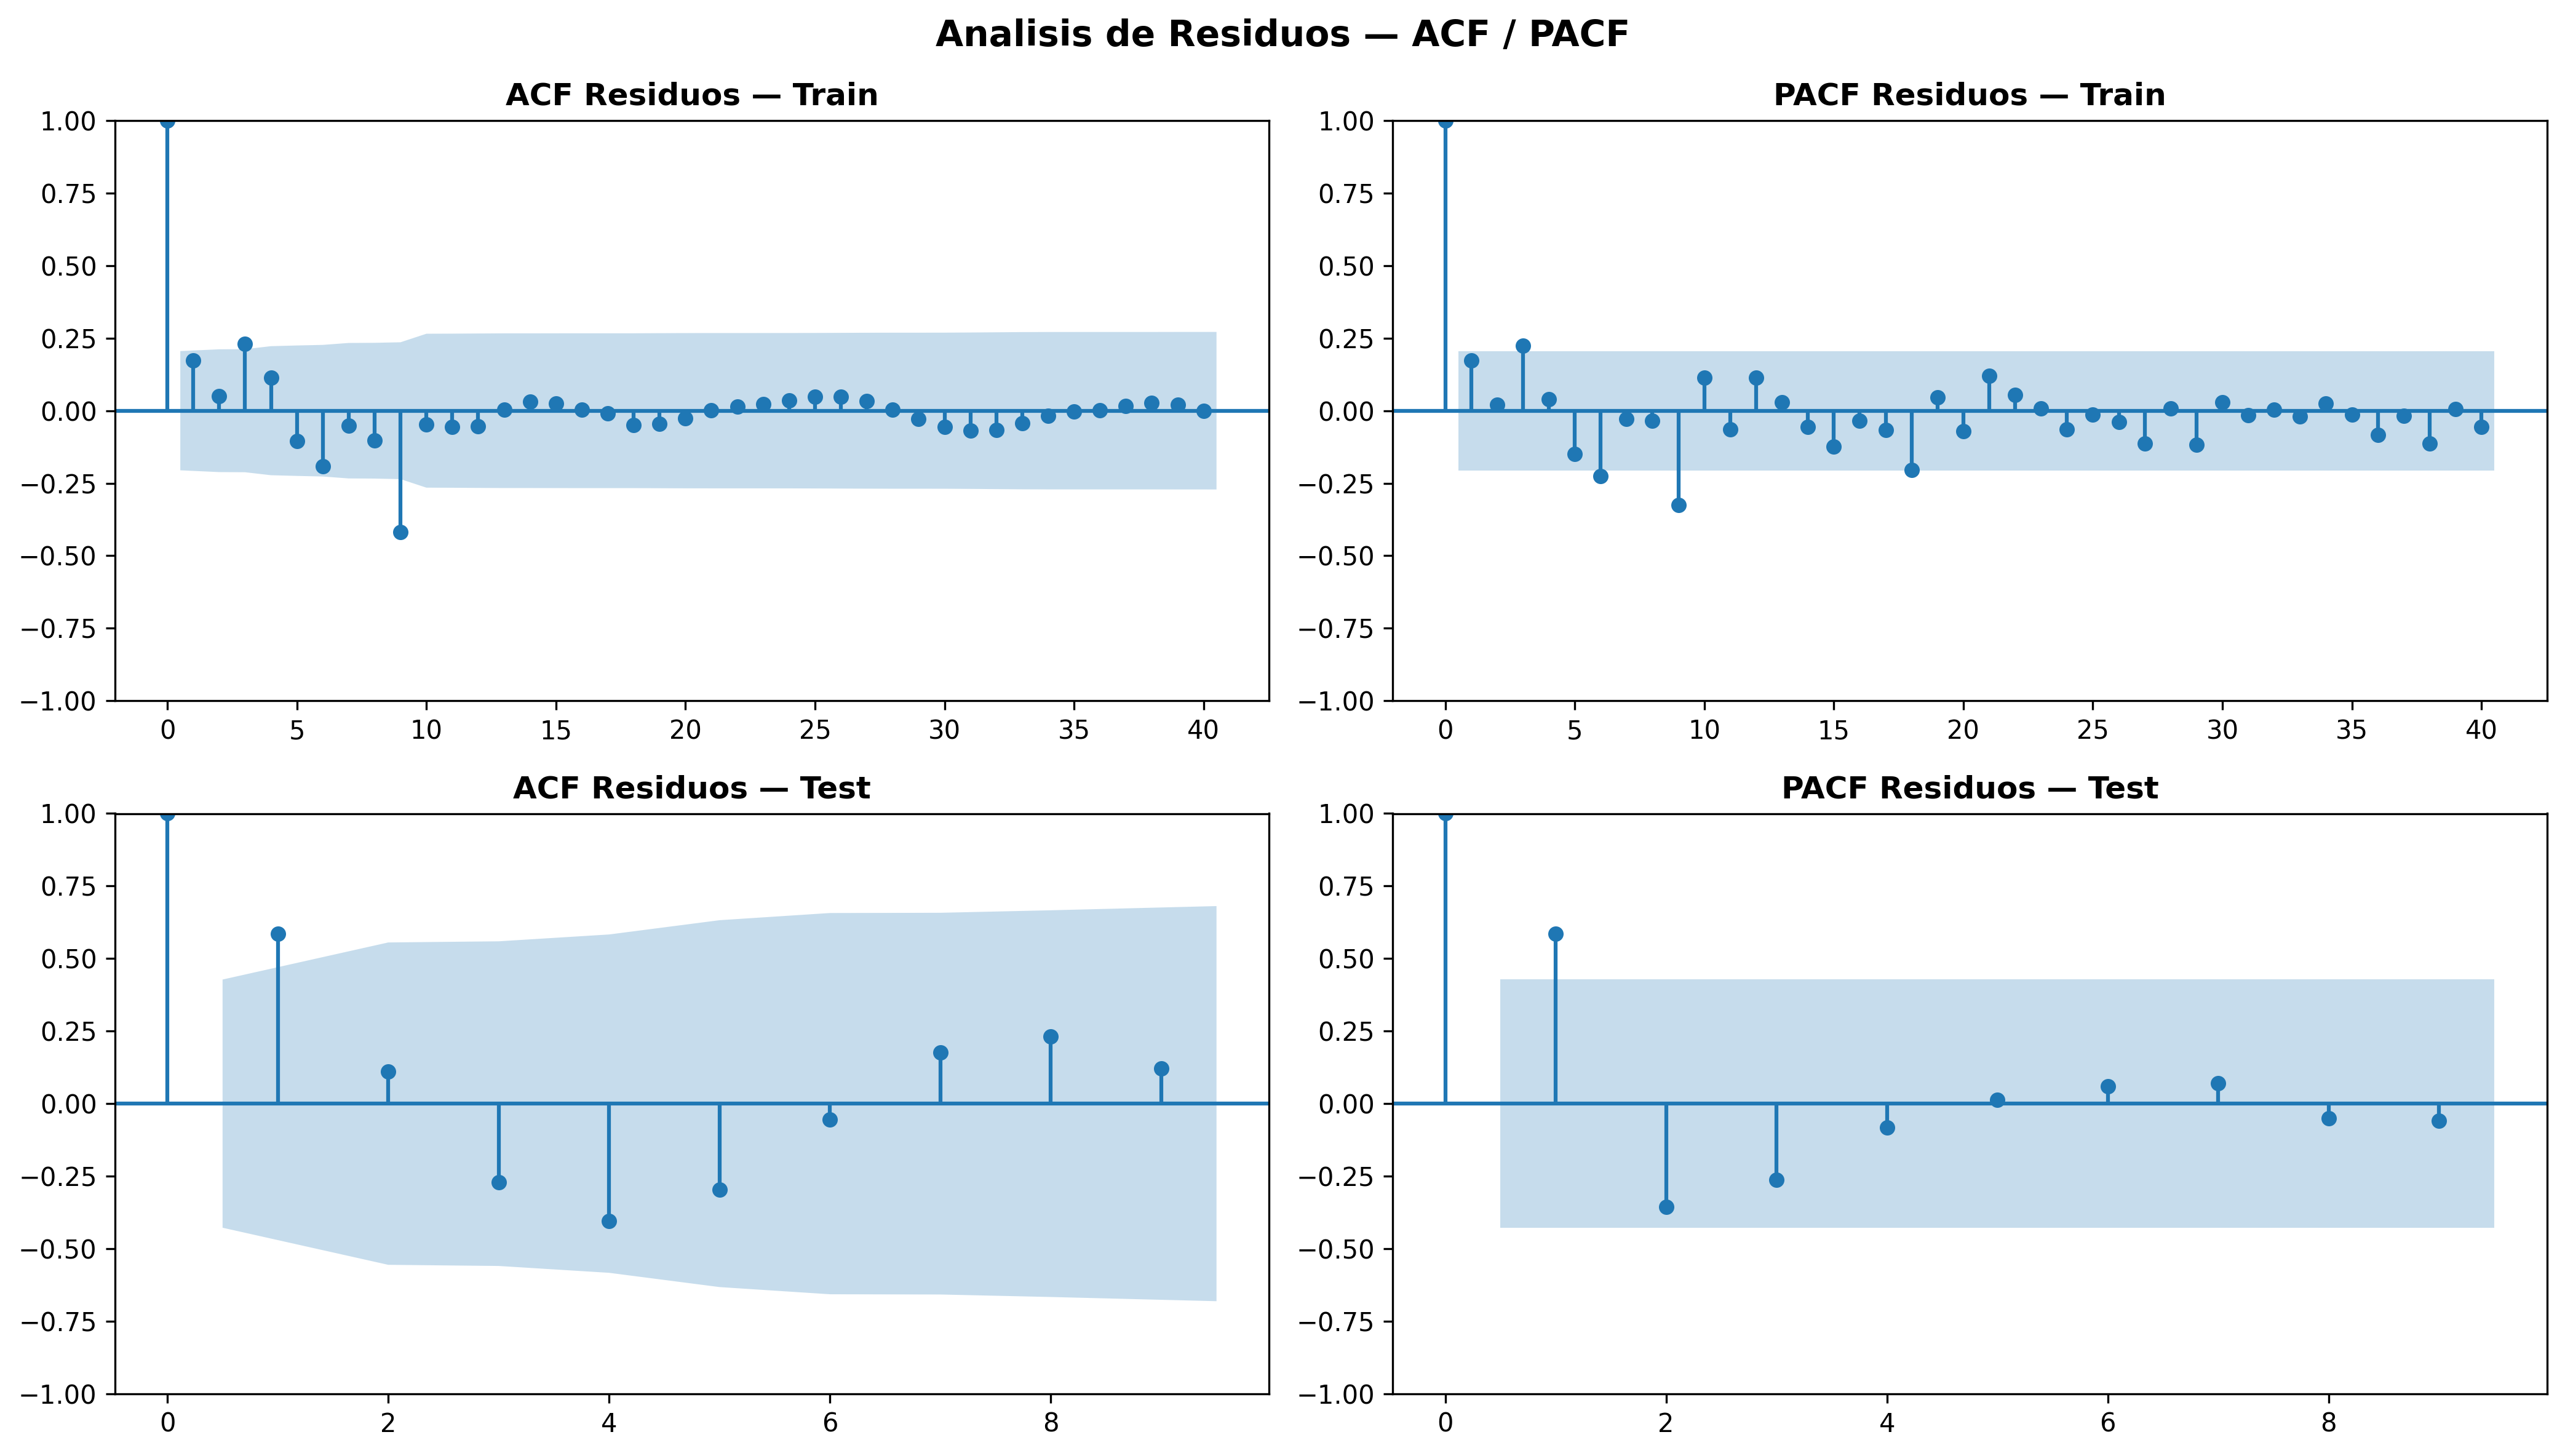
\includegraphics[width=\textwidth]{predicciones/prediccion_cemento_lstm/resultados_sin_covid/residuos_acf_pacf.png}
    \caption{ACF y PACF de los residuos del modelo LSTM para cemento.}
    \label{fig:lstm_cemento_acf_residuos}
\end{figure}

\justify
El test de Ljung-Box sobre los residuos del conjunto de prueba arrojó un $p$-valor de 0,017 con 10 rezagos y de 0,042 con 20 rezagos, ambos por debajo del umbral de 0,05. Esto indica la presencia de autocorrelación residual estadísticamente significativa, aunque los $p$-valores son cercanos al límite de significancia. Este resultado sugiere que el modelo deja alguna estructura temporal sin capturar en sus residuos, lo que debe tenerse en cuenta al interpretar los intervalos de confianza estimados por Monte Carlo Dropout.

\clearpage
\subsubsection{Pronóstico a 24 Meses --- Escenario sin Pandemia}

\justify
Se generó el pronóstico del precio del cemento para los 24 meses comprendidos entre agosto de 2025 y julio de 2027, con la variable \texttt{Cuarentena\_Covid} fijada en 0 durante todo el horizonte de predicción, simulando condiciones normales de mercado.

\begin{figure}[htbp]
    \centering
    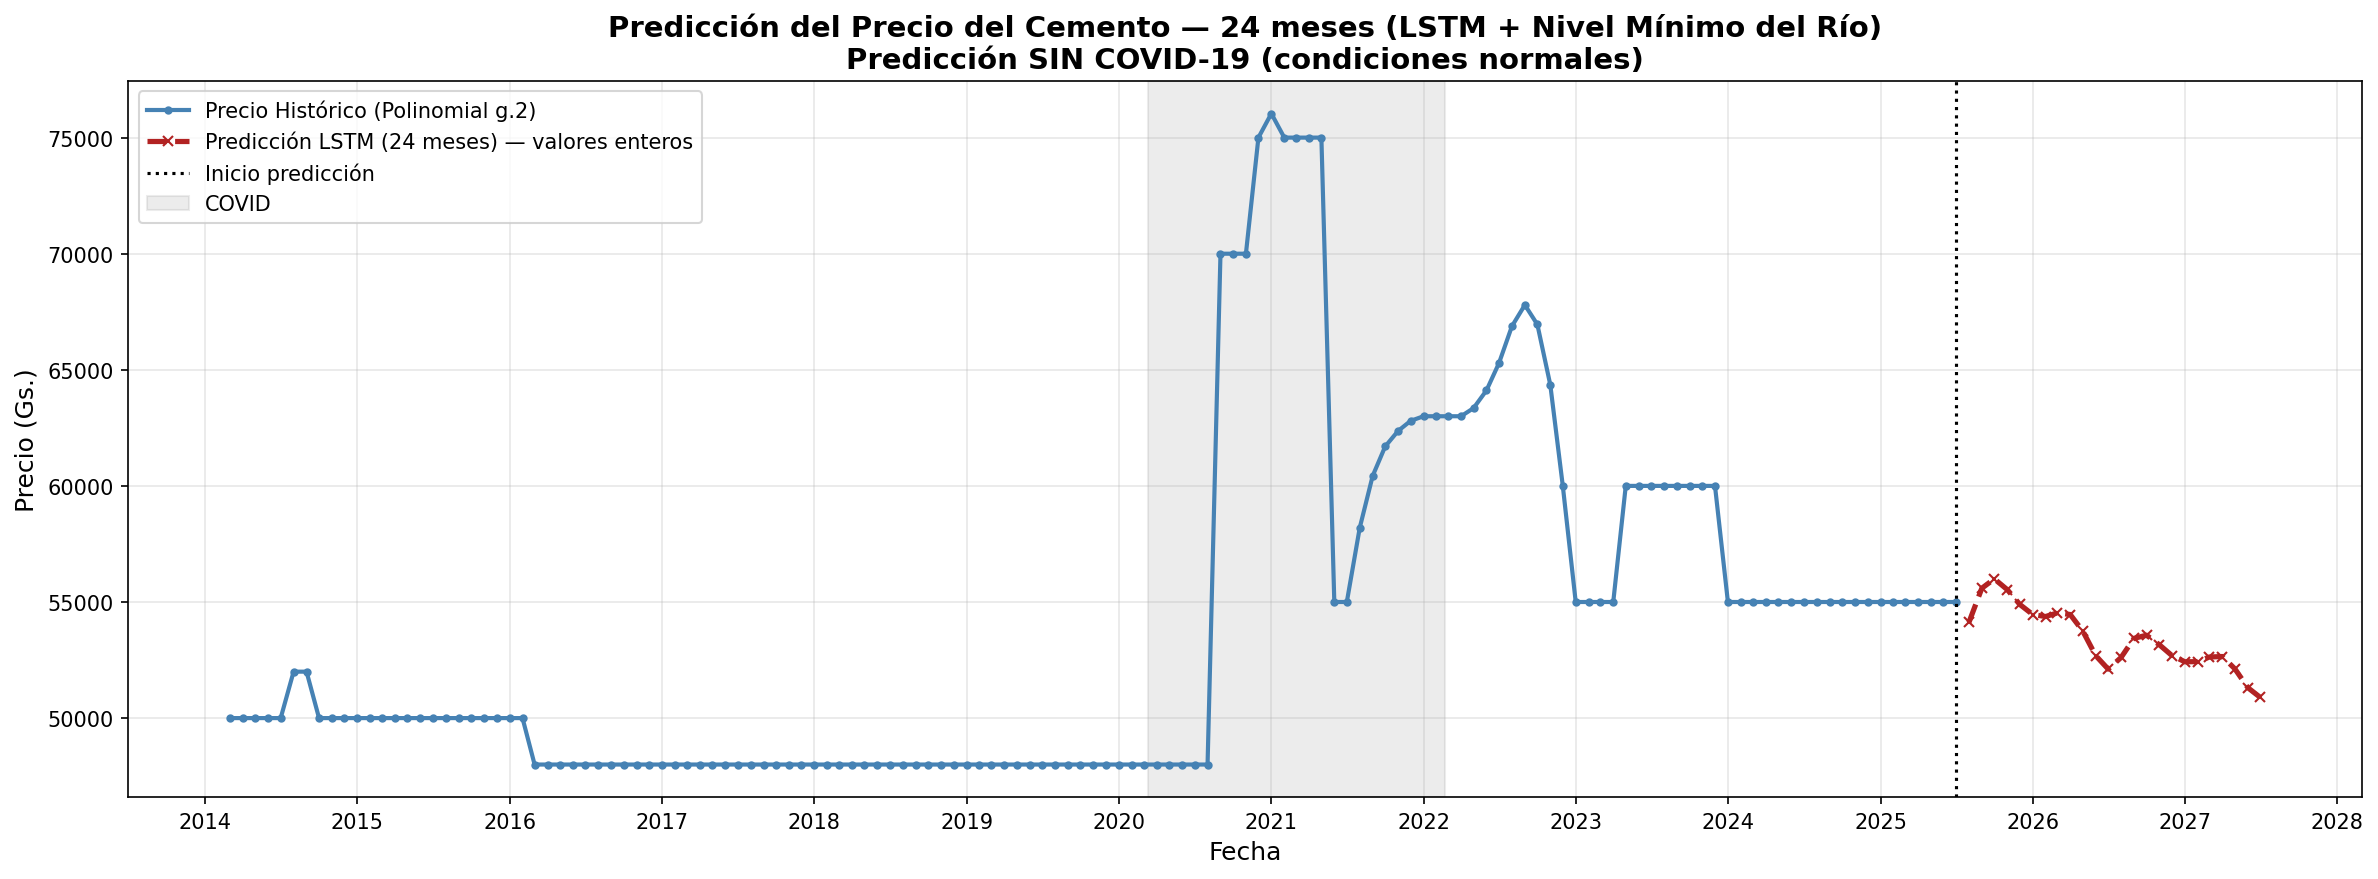
\includegraphics[width=\textwidth]{predicciones/prediccion_cemento_lstm/resultados_sin_covid/final_06_prediccion_futura_completa.png}
    \caption{Pronóstico LSTM a 24 meses del precio del cemento --- escenario sin pandemia, con intervalos de confianza al 95\,\%.}
    \label{fig:lstm_cemento_pred_sin_covid}
\end{figure}

\begin{figure}[htbp]
    \centering
    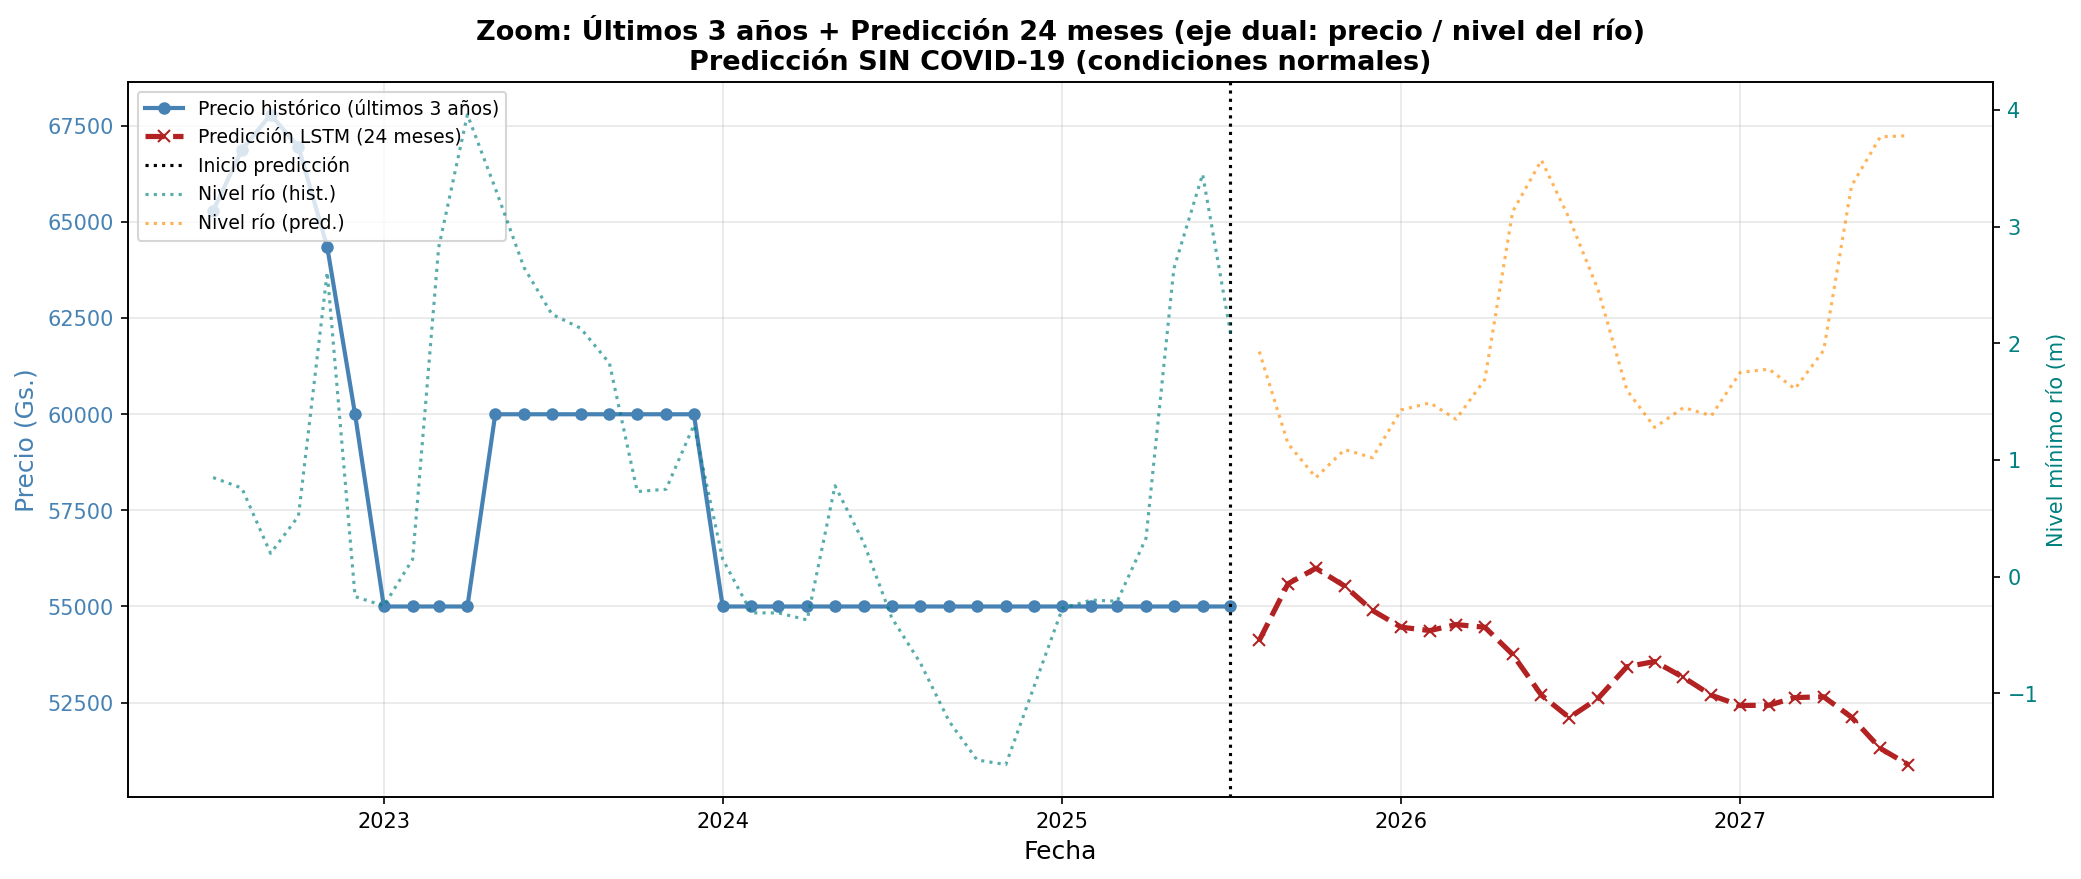
\includegraphics[width=\textwidth]{predicciones/prediccion_cemento_lstm/resultados_sin_covid/final_07_prediccion_zoom_dual.png}
    \caption{Detalle de la transición entre datos históricos y pronóstico LSTM del cemento --- escenario sin pandemia.}
    \label{fig:lstm_cemento_zoom_sin_covid}
\end{figure}

\begin{figure}[htbp]
    \centering
    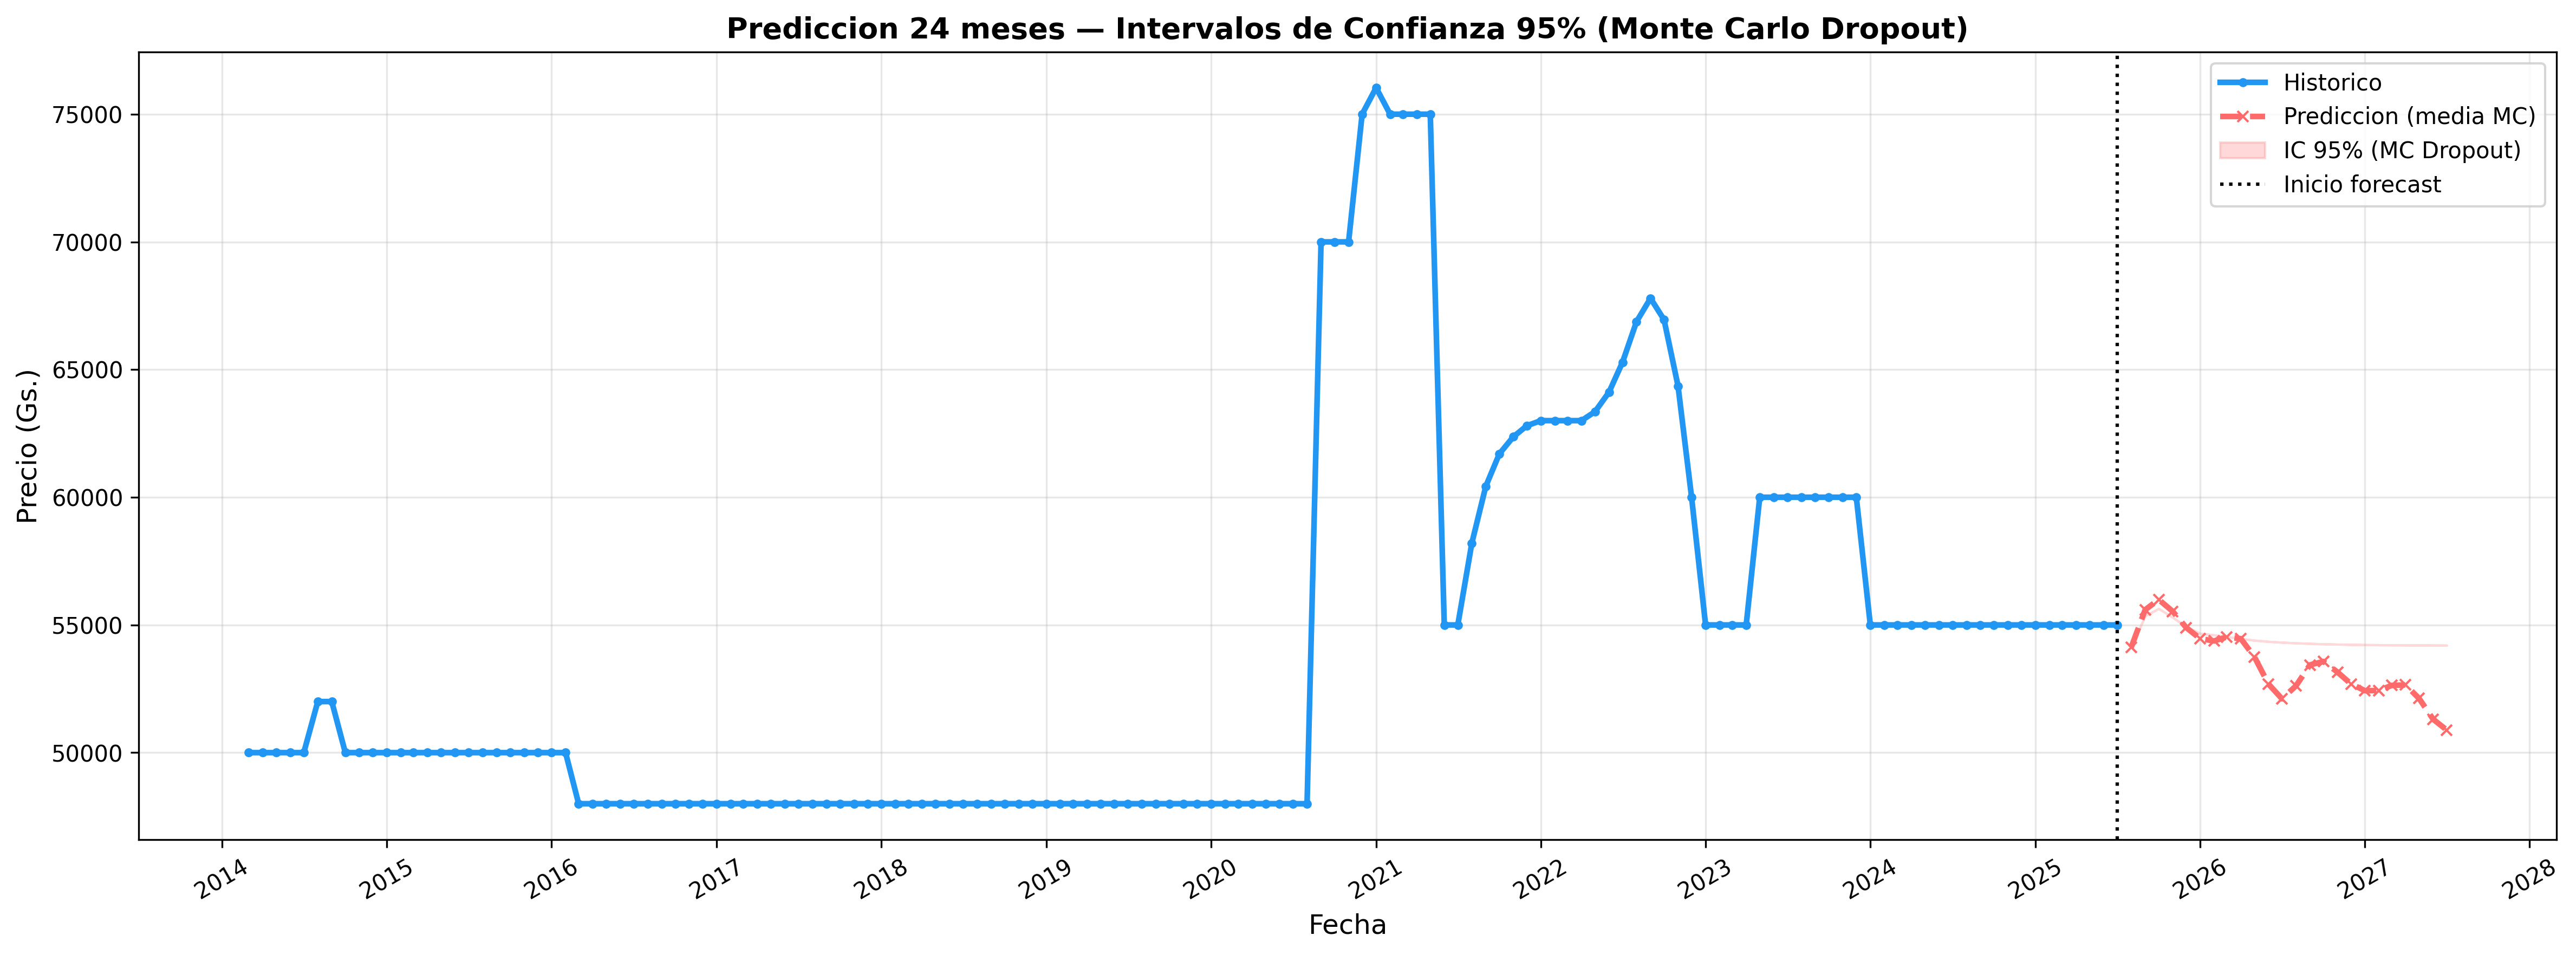
\includegraphics[width=\textwidth]{predicciones/prediccion_cemento_lstm/resultados_sin_covid/forecast_ic_monte_carlo.png}
    \caption{Intervalo de confianza Monte Carlo Dropout del pronóstico LSTM para cemento --- escenario sin pandemia.}
    \label{fig:lstm_cemento_ic_mc_sin_covid}
\end{figure}

\justify
Bajo el escenario sin pandemia, el rango de precios predicho se sitúa entre Gs.~50.888 y Gs.~55.996 a lo largo del horizonte de 24 meses, reflejando una tendencia estable con leve tendencia descendente a partir del primer año de proyección.

\clearpage
\subsubsection{Pronóstico a 24 Meses --- Escenario con Efecto Pandémico}

\justify
En este escenario, el mismo modelo entrenado se utilizó para generar el pronóstico con la variable \texttt{Cuarentena\_Covid} activada (valor 1) durante todo el horizonte de predicción. Este escenario hipotético permite evaluar cómo el modelo LSTM responde ante disrupciones prolongadas de tipo pandémico.

\begin{figure}[htbp]
    \centering
    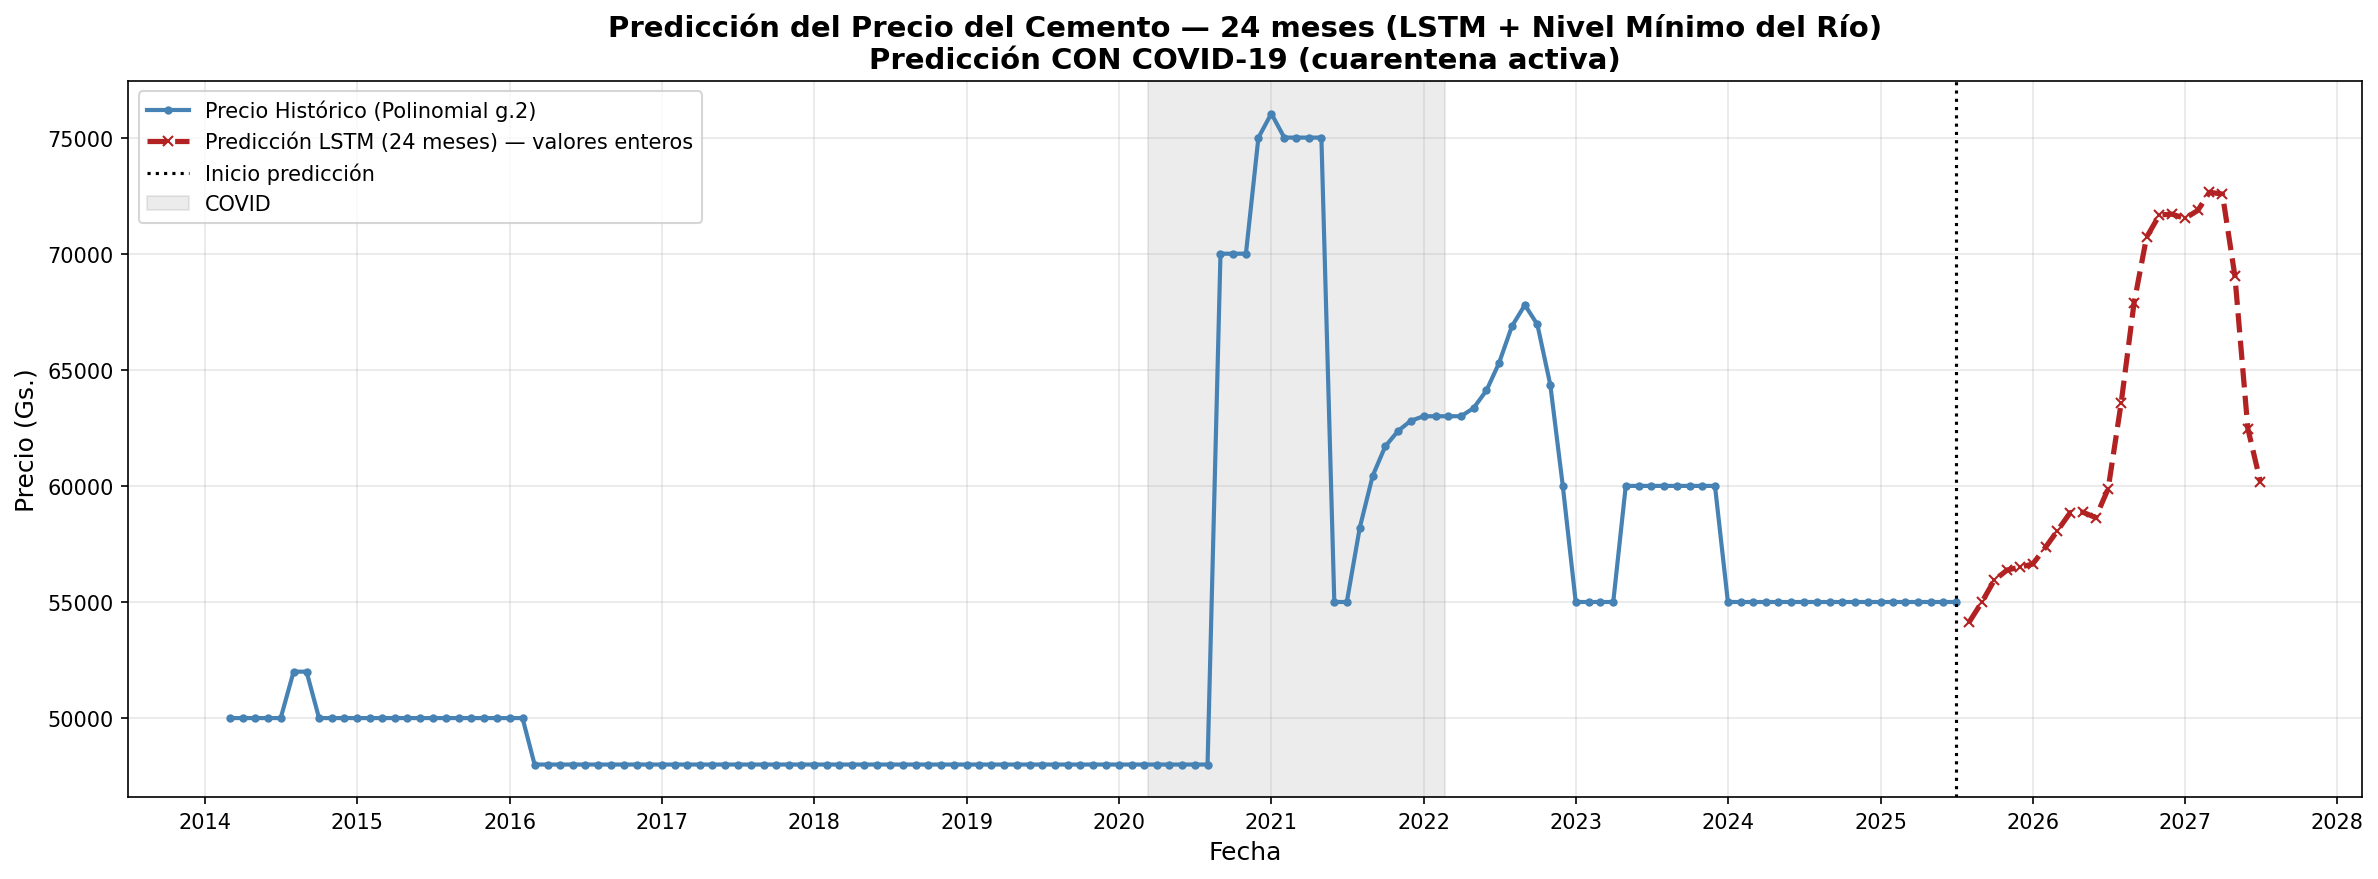
\includegraphics[width=\textwidth]{predicciones/prediccion_cemento_lstm/resultados_con_covid/final_06_prediccion_futura_completa.png}
    \caption{Pronóstico LSTM a 24 meses del precio del cemento --- escenario con efecto pandémico, con intervalos de confianza al 95\,\%.}
    \label{fig:lstm_cemento_pred_con_covid}
\end{figure}

\begin{figure}[htbp]
    \centering
    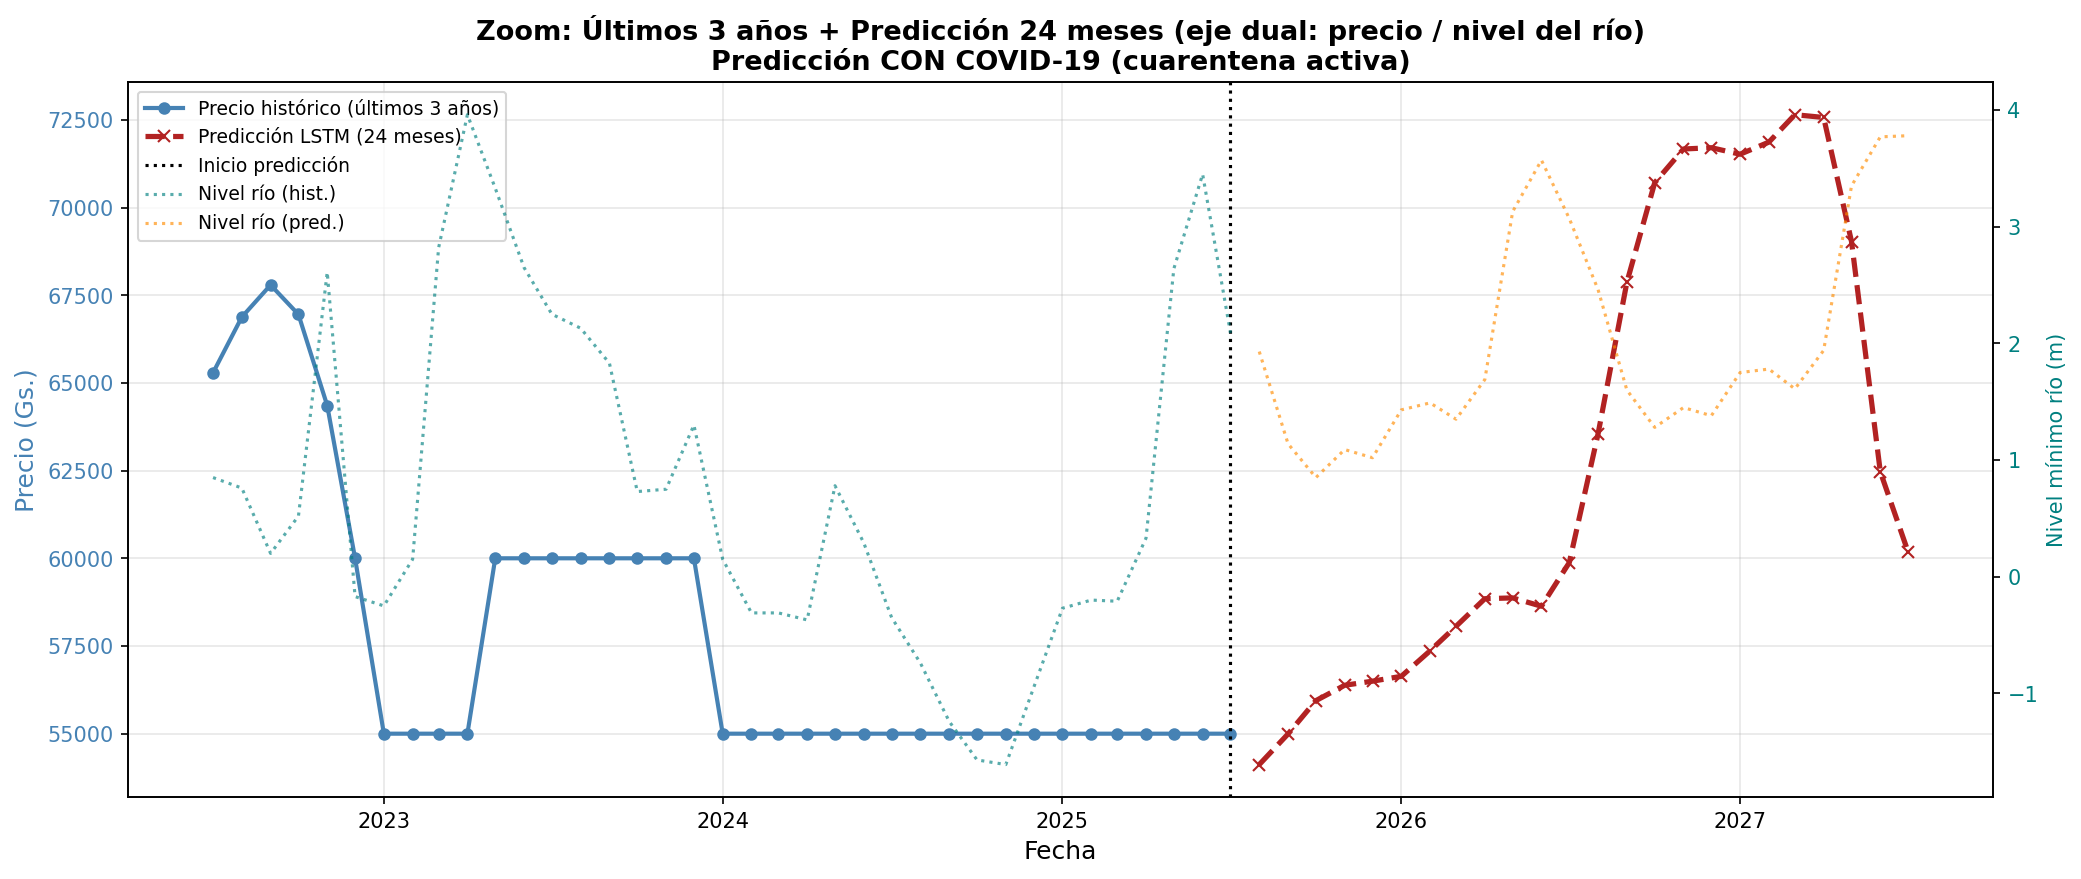
\includegraphics[width=\textwidth]{predicciones/prediccion_cemento_lstm/resultados_con_covid/final_07_prediccion_zoom_dual.png}
    \caption{Detalle de la transición entre datos históricos y pronóstico LSTM del cemento --- escenario con efecto pandémico.}
    \label{fig:lstm_cemento_zoom_con_covid}
\end{figure}

\begin{figure}[htbp]
    \centering
    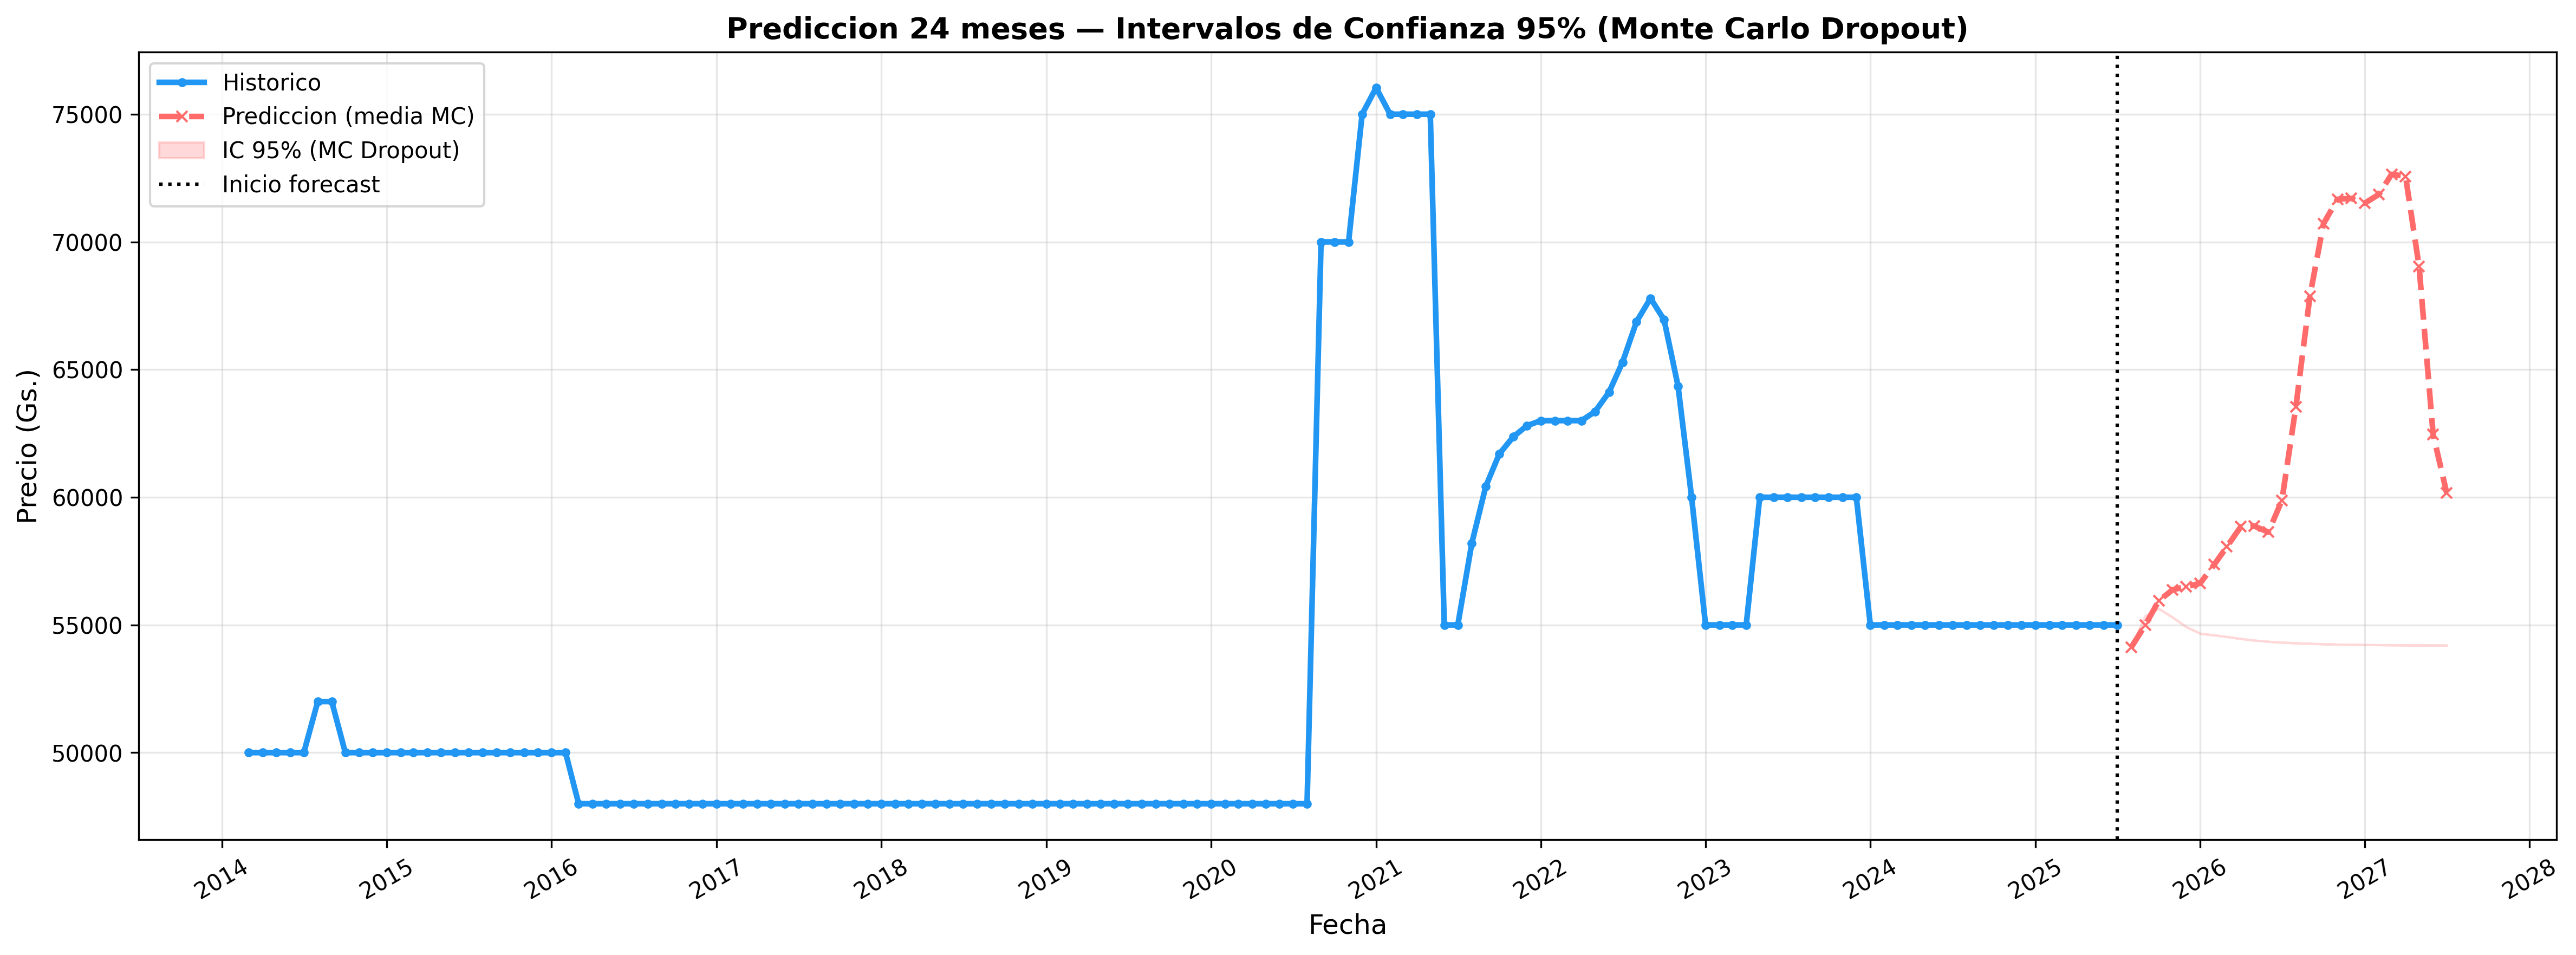
\includegraphics[width=\textwidth]{predicciones/prediccion_cemento_lstm/resultados_con_covid/forecast_ic_monte_carlo.png}
    \caption{Intervalo de confianza Monte Carlo Dropout del pronóstico LSTM para cemento --- escenario con efecto pandémico.}
    \label{fig:lstm_cemento_ic_mc_con_covid}
\end{figure}

\justify
Bajo el escenario con efecto pandémico, el rango de precios predicho se sitúa entre Gs.~54.119 y Gs.~72.646, considerablemente más elevado y con mayor dispersión que el escenario sin pandemia. La diferencia entre ambos escenarios revela que el modelo LSTM asigna un efecto alcista significativo a la variable de cuarentena: el precio máximo predicho pasa de Gs.~55.996 (sin pandemia) a Gs.~72.646 (con pandemia), un incremento del 29,7\,\% en el límite superior del rango. Este comportamiento es consistente con lo observado durante la pandemia real de 2020--2021, donde las disrupciones en la cadena de suministro provocaron aumentos sostenidos en los precios del cemento.

% ============================================================
%  LADRILLO
% ============================================================
\clearpage
\subsection{Predicción del Precio del Ladrillo}

\justify
Para el ladrillo, la búsqueda de hiperparámetros con Optuna identificó arquitecturas diferentes para cada escenario. El escenario sin pandemia fue optimizado con 261 pruebas durante 480,9 minutos y convergió a una arquitectura LSTM bidireccional; el escenario con pandemia, con una sola prueba de configuración, seleccionó una arquitectura unidireccional más compacta. Dado que los modelos son distintos, cada escenario se presenta con su propia descripción completa: hiperparámetros, entrenamiento, evaluación y pronóstico.

\subsubsection{Análisis Exploratorio de la Serie}

\begin{figure}[htbp]
    \centering
    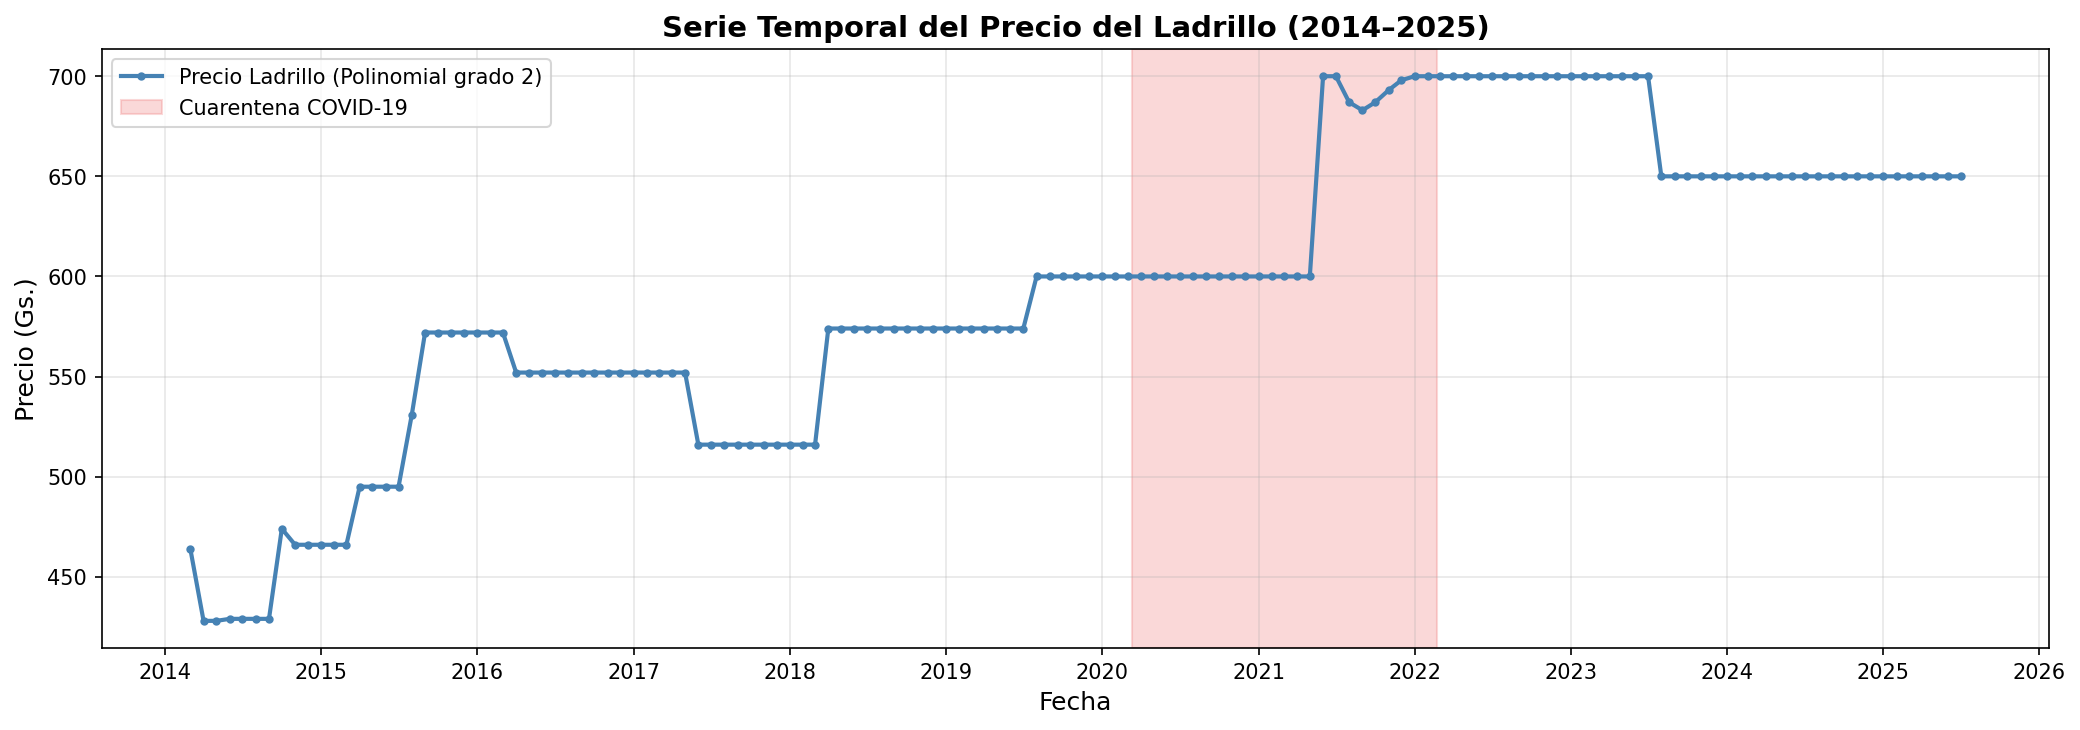
\includegraphics[width=\textwidth]{predicciones/prediccion_ladrillo_lstm/resultados_sin_covid/eda_01_serie_precios_ladrillo.png}
    \caption{Serie histórica mensual del precio del ladrillo (Gs.), período 2014--2025.}
    \label{fig:lstm_ladrillo_eda_serie}
\end{figure}

\begin{figure}[htbp]
    \centering
    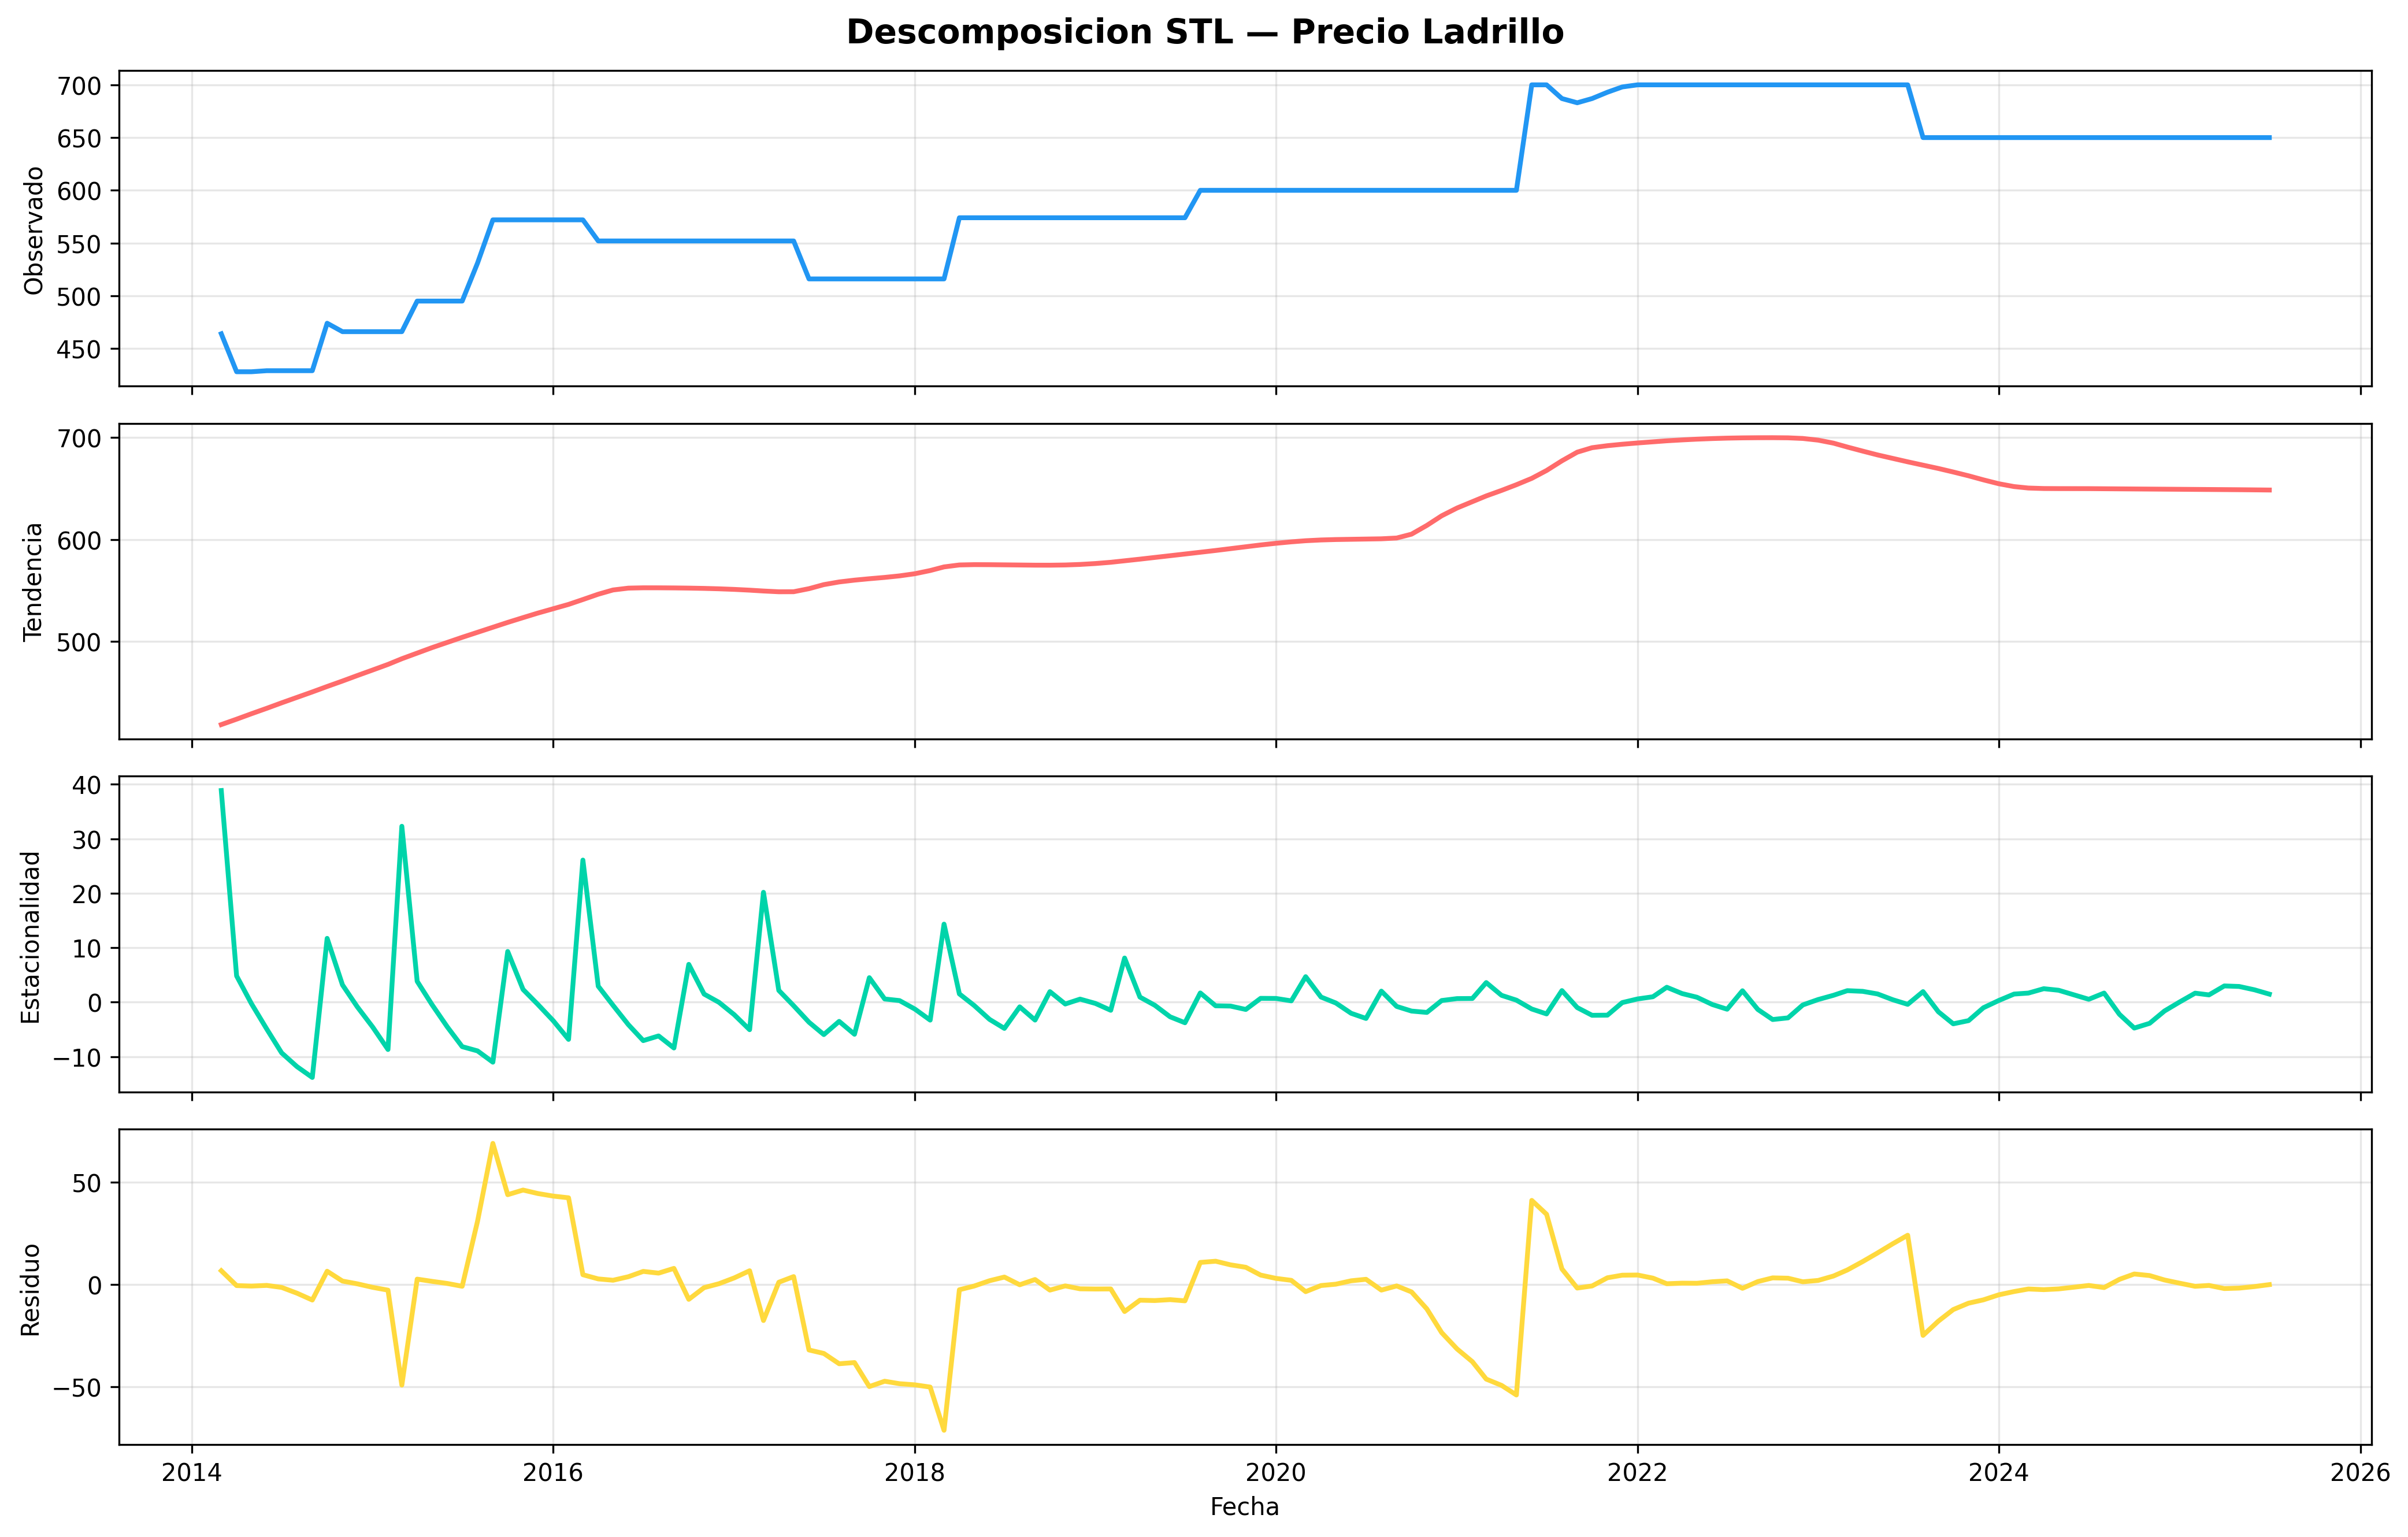
\includegraphics[width=\textwidth]{predicciones/prediccion_ladrillo_lstm/resultados_sin_covid/eda_stl_decomposition.png}
    \caption{Descomposición STL de la serie del precio del ladrillo: tendencia, estacionalidad y residuo.}
    \label{fig:lstm_ladrillo_eda_stl}
\end{figure}

\begin{figure}[htbp]
    \centering
    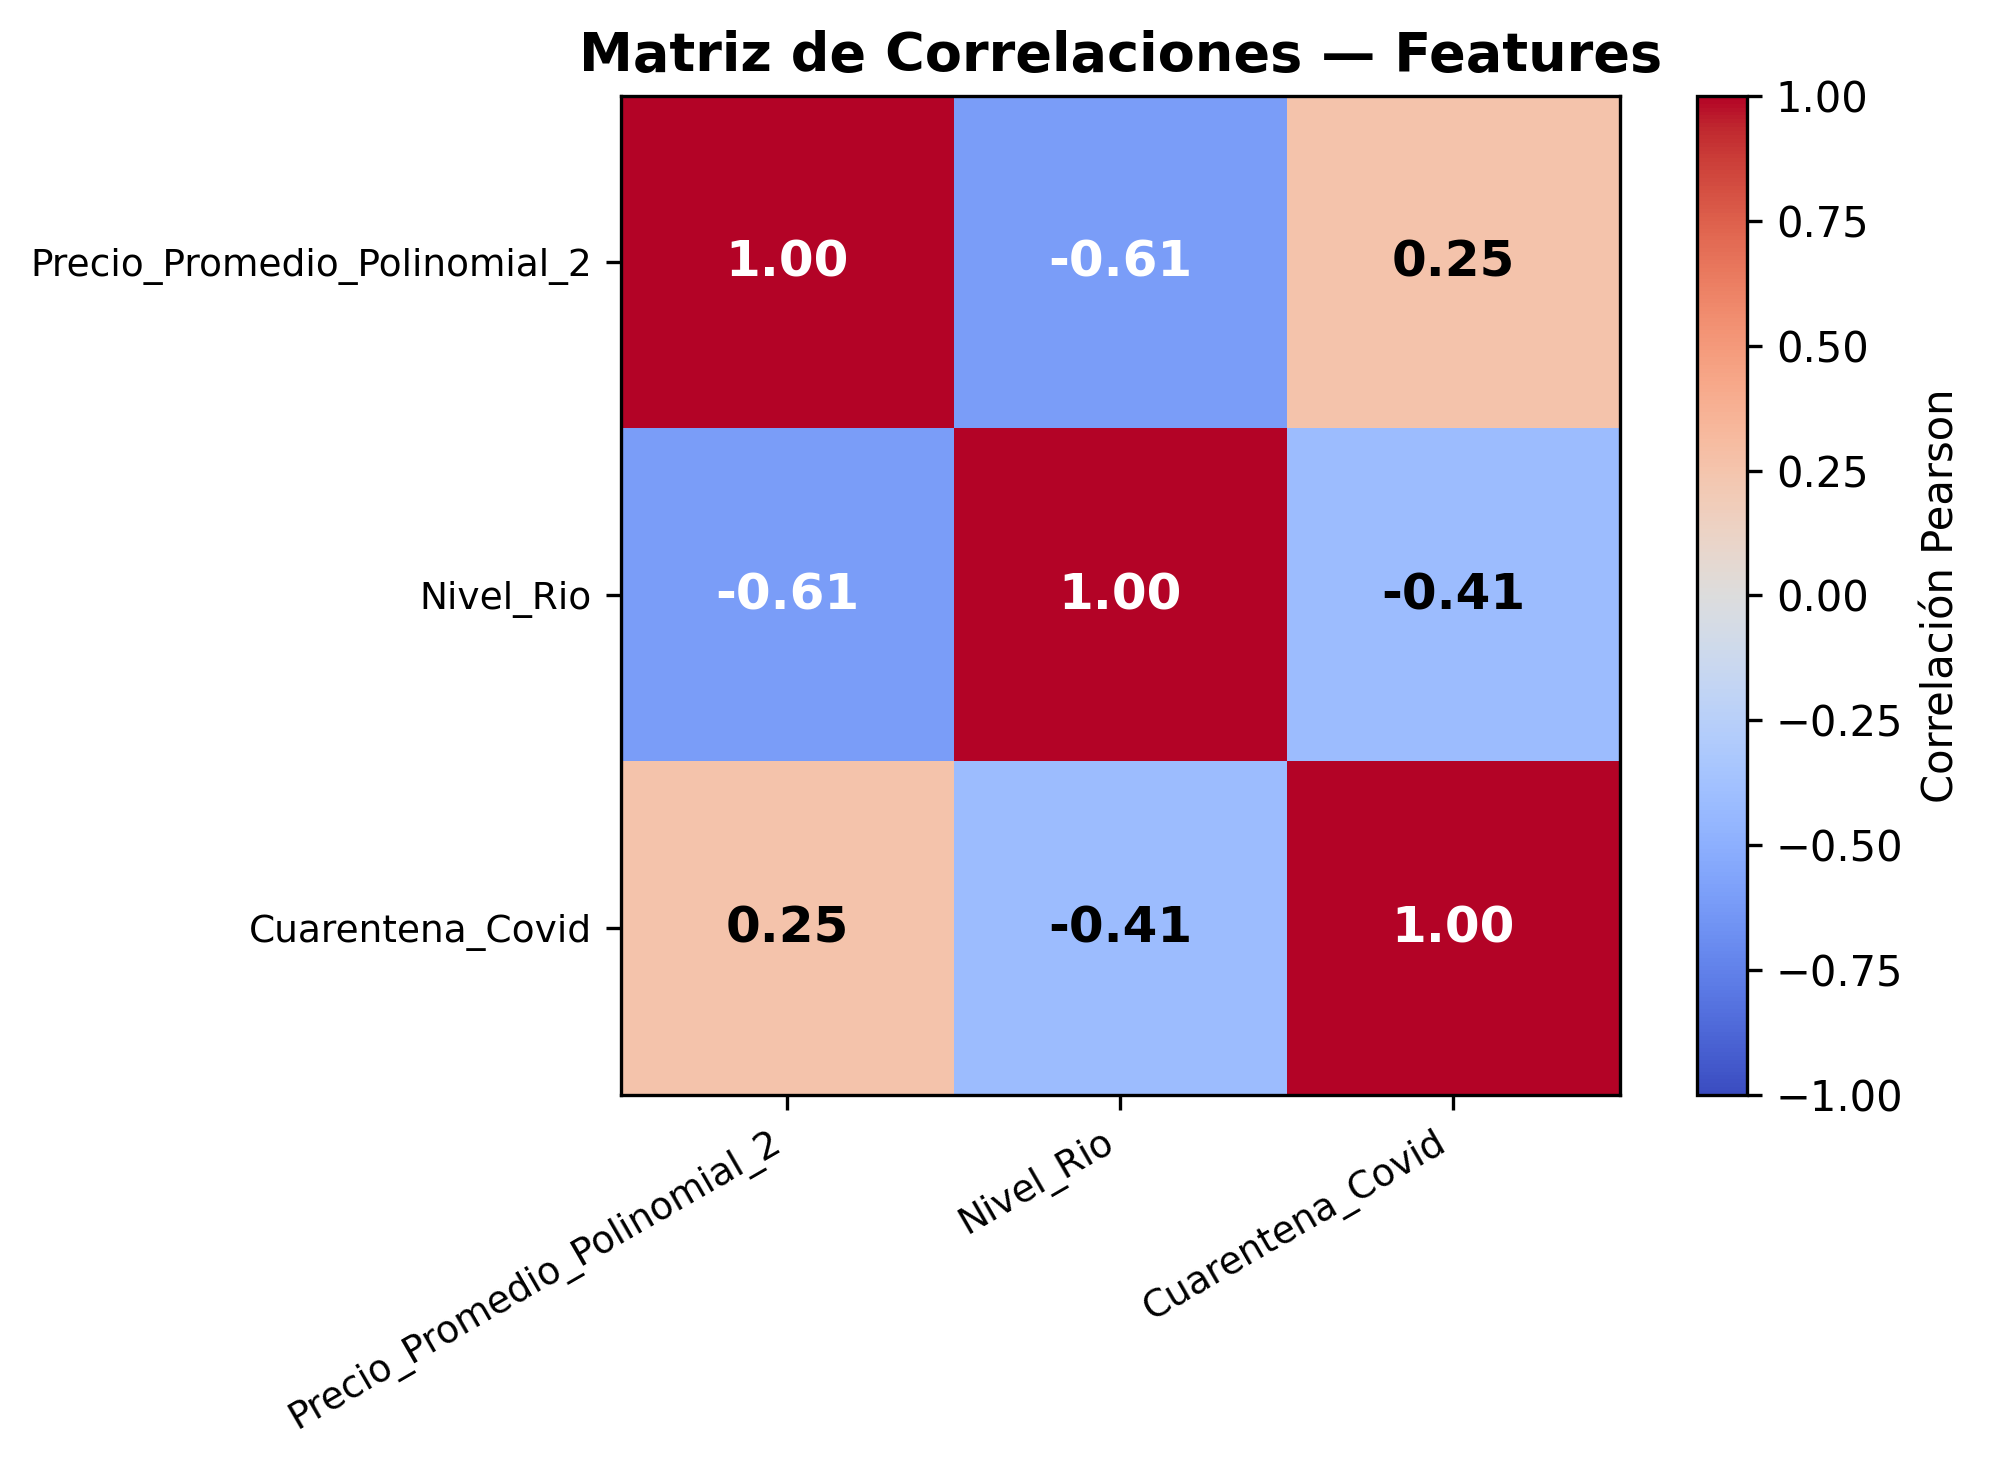
\includegraphics[width=\textwidth]{predicciones/prediccion_ladrillo_lstm/resultados_sin_covid/eda_correlaciones_heatmap.png}
    \caption{Mapa de calor de correlaciones entre las variables de entrada del modelo LSTM para ladrillo.}
    \label{fig:lstm_ladrillo_eda_corr}
\end{figure}

% ------ LADRILLO SIN COVID ------
\clearpage
\subsubsection{Escenario sin Efecto Pandémico}

\paragraph{Hiperparámetros y Arquitectura}

\justify
La búsqueda con Optuna (261 ensayos, 480,9 min) convergió a una arquitectura LSTM \textbf{bidireccional} con una capa de 64 unidades ocultas, lo que permite al modelo procesar la secuencia en ambas direcciones y capturar dependencias pasadas y futuras dentro de la ventana de entrada. Se incorporaron \textit{dropout} de 0,2 y \textit{dropout} recurrente de 0,05 como mecanismos de regularización, junto con el optimizador Adam, tasa de aprendizaje $\text{lr}=0{,}006317$, regularización L2 $\lambda=7{,}35 \times 10^{-6}$, \textit{lookback} de 4 meses y \textit{scheduler} StepLR. La Tabla~\ref{tab:lstm_ladrillo_sc_hiper} detalla estos parámetros.

\begin{table}[htbp]
\centering
\caption{Hiperparámetros óptimos del modelo LSTM para ladrillo --- escenario sin pandemia (Optuna: 261 ensayos).}
\label{tab:lstm_ladrillo_sc_hiper}
\begin{tabular}{ll}
\toprule
\textbf{Hiperparámetro} & \textbf{Valor} \\
\midrule
Capas LSTM          & 1 \\
Unidades ocultas    & 64 \\
Bidireccional       & Sí \\
Dropout             & 0,2 \\
Dropout recurrente  & 0,05 \\
Optimizador         & Adam \\
Tasa de aprendizaje & 0,006317 \\
Regularización L2   & $7{,}35 \times 10^{-6}$ \\
Lookback            & 4 meses \\
Batch size          & 4 \\
Scheduler           & StepLR \\
Parámetros entrenables & 36.993 \\
\bottomrule
\end{tabular}
\end{table}

\paragraph{Curva de Aprendizaje}

\begin{figure}[htbp]
    \centering
    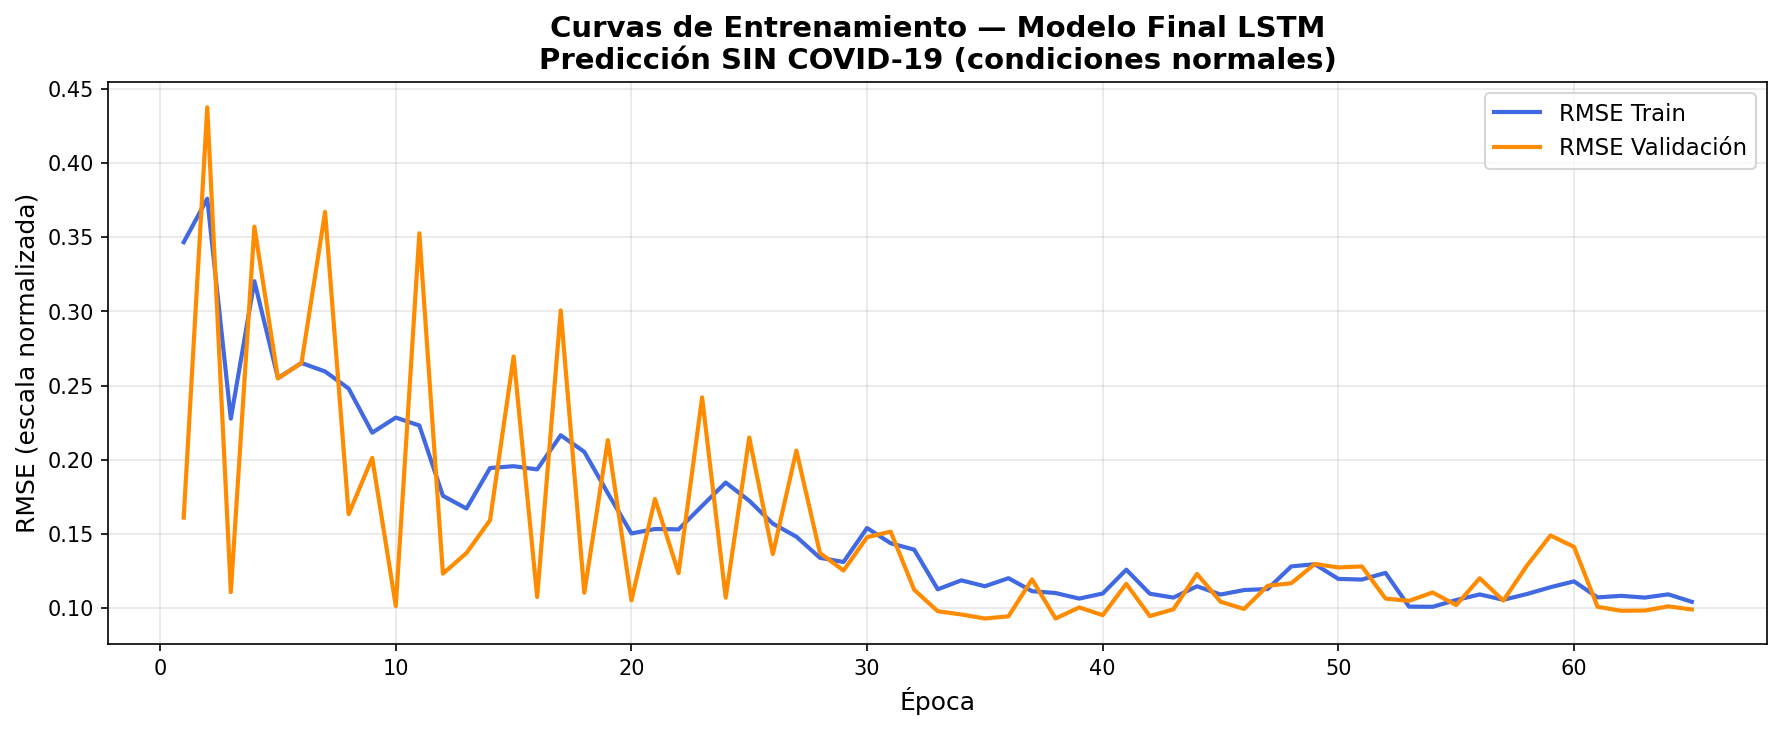
\includegraphics[width=0.85\textwidth]{predicciones/prediccion_ladrillo_lstm/resultados_sin_covid/final_01_curvas_entrenamiento.png}
    \caption{Curva de aprendizaje del modelo LSTM para ladrillo --- escenario sin pandemia.}
    \label{fig:lstm_ladrillo_curva_sc}
\end{figure}

\paragraph{Métricas de Evaluación}

\begin{table}[htbp]
\centering
\caption{Desempeño del modelo LSTM para ladrillo --- escenario sin pandemia: RMSE en train, val y test.}
\label{tab:lstm_ladrillo_sc_metricas}
\begin{tabular}{lrrr}
\toprule
\textbf{Métrica} & \textbf{Train} & \textbf{Val} & \textbf{Test} \\
\midrule
RMSE (Gs.) & 13,76 & 12,53 & 6,32 \\
\bottomrule
\end{tabular}
\end{table}

\justify
El RMSE de prueba de 6,32~Gs.\ representa un error relativo inferior al 2\,\% del rango histórico de la serie (Gs.~428--700), evidenciando una capacidad predictiva excelente. El hecho de que sea incluso menor que el de entrenamiento (13,76~Gs.) indica que el período de prueba presenta menor volatilidad que el período de entrenamiento.

\paragraph{Evaluación sobre el Conjunto de Prueba}

\begin{figure}[htbp]
    \centering
    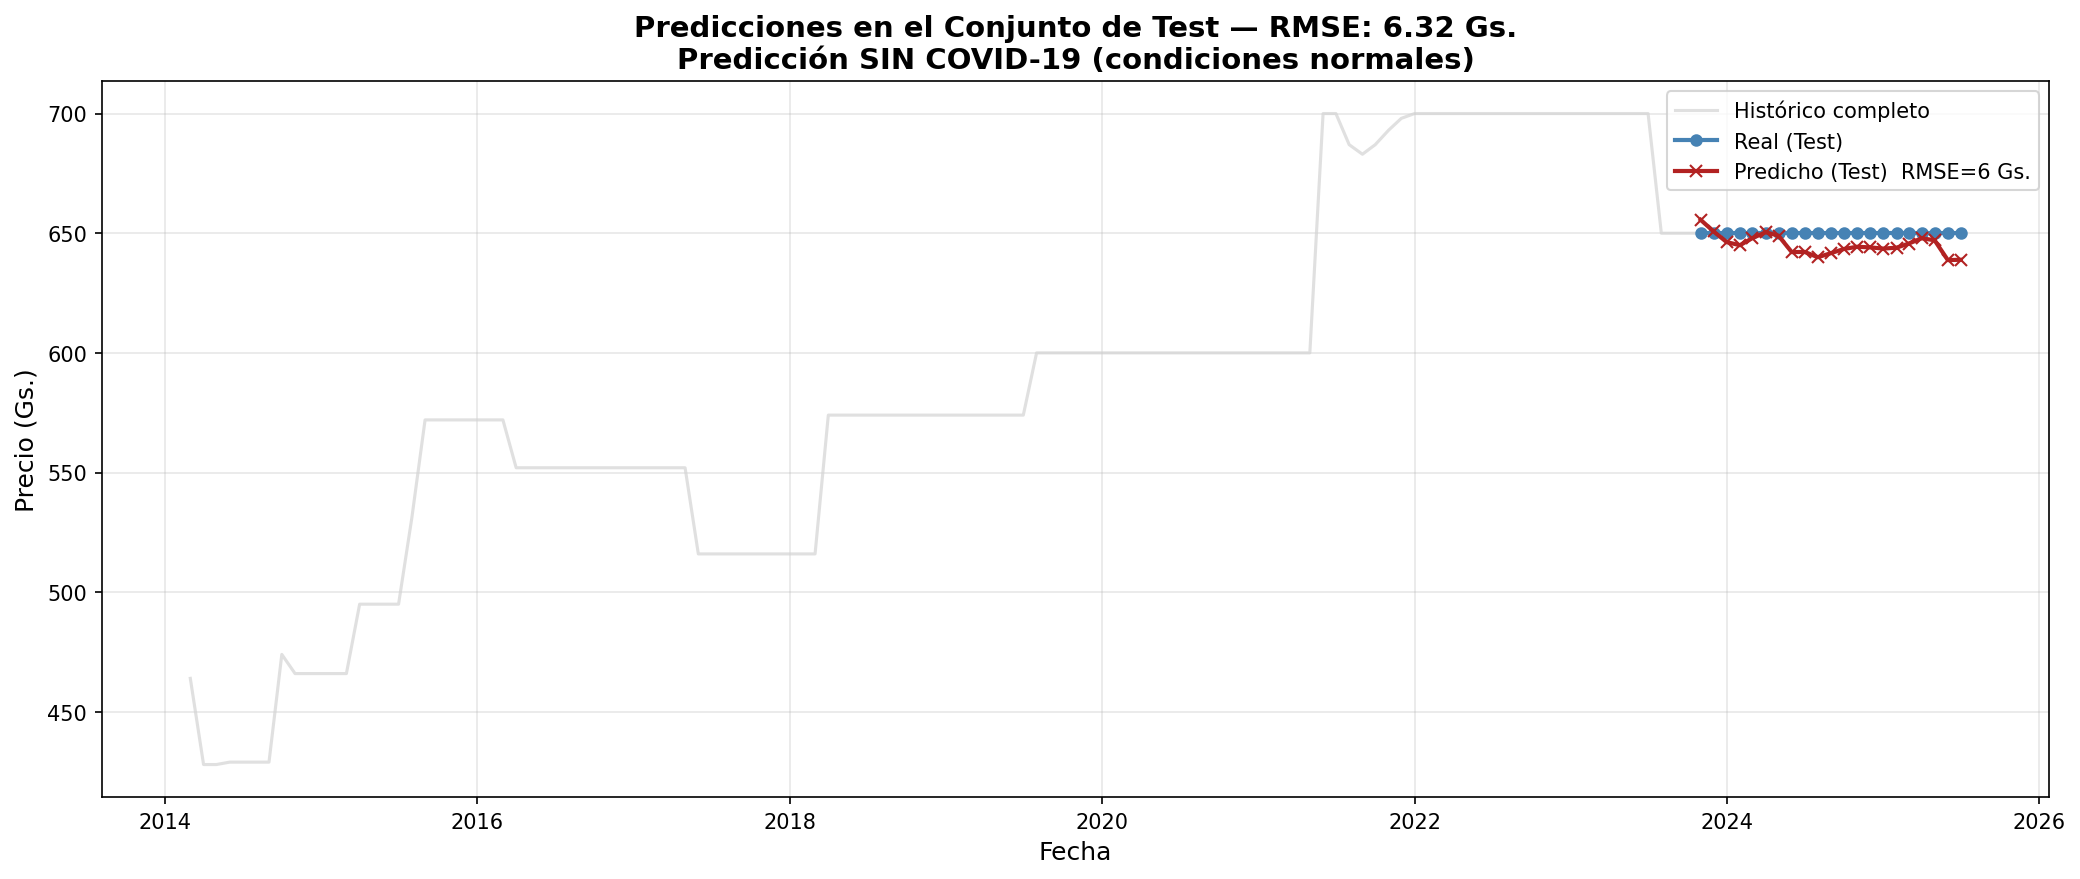
\includegraphics[width=\textwidth]{predicciones/prediccion_ladrillo_lstm/resultados_sin_covid/final_02_prediccion_test_serie.png}
    \caption{Predicción LSTM vs.\ valores reales del precio del ladrillo --- escenario sin pandemia, conjunto de prueba.}
    \label{fig:lstm_ladrillo_test_sc}
\end{figure}

\begin{figure}[htbp]
    \centering
    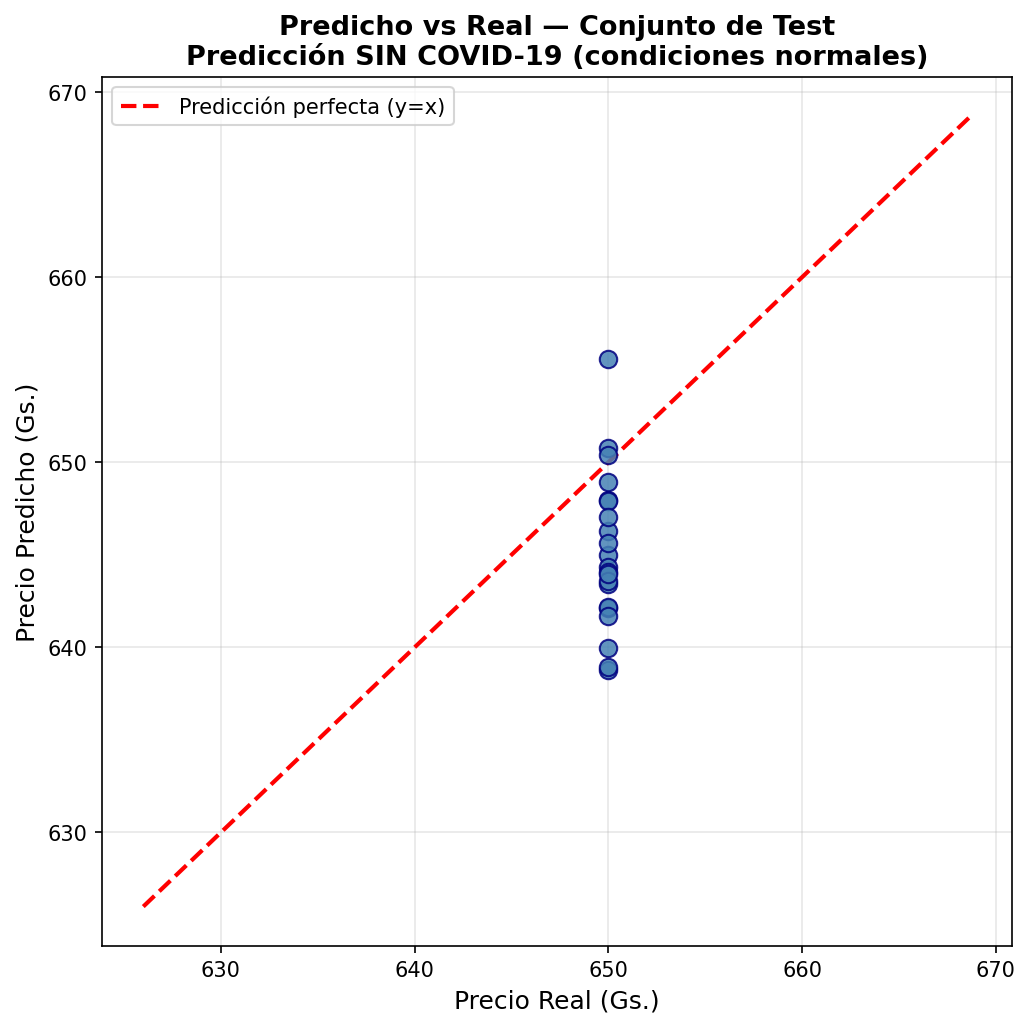
\includegraphics[width=0.7\textwidth]{predicciones/prediccion_ladrillo_lstm/resultados_sin_covid/final_03_scatter_test.png}
    \caption{Diagrama de dispersión: precio predicho vs.\ real del ladrillo --- escenario sin pandemia.}
    \label{fig:lstm_ladrillo_scatter_sc}
\end{figure}

\begin{figure}[htbp]
    \centering
    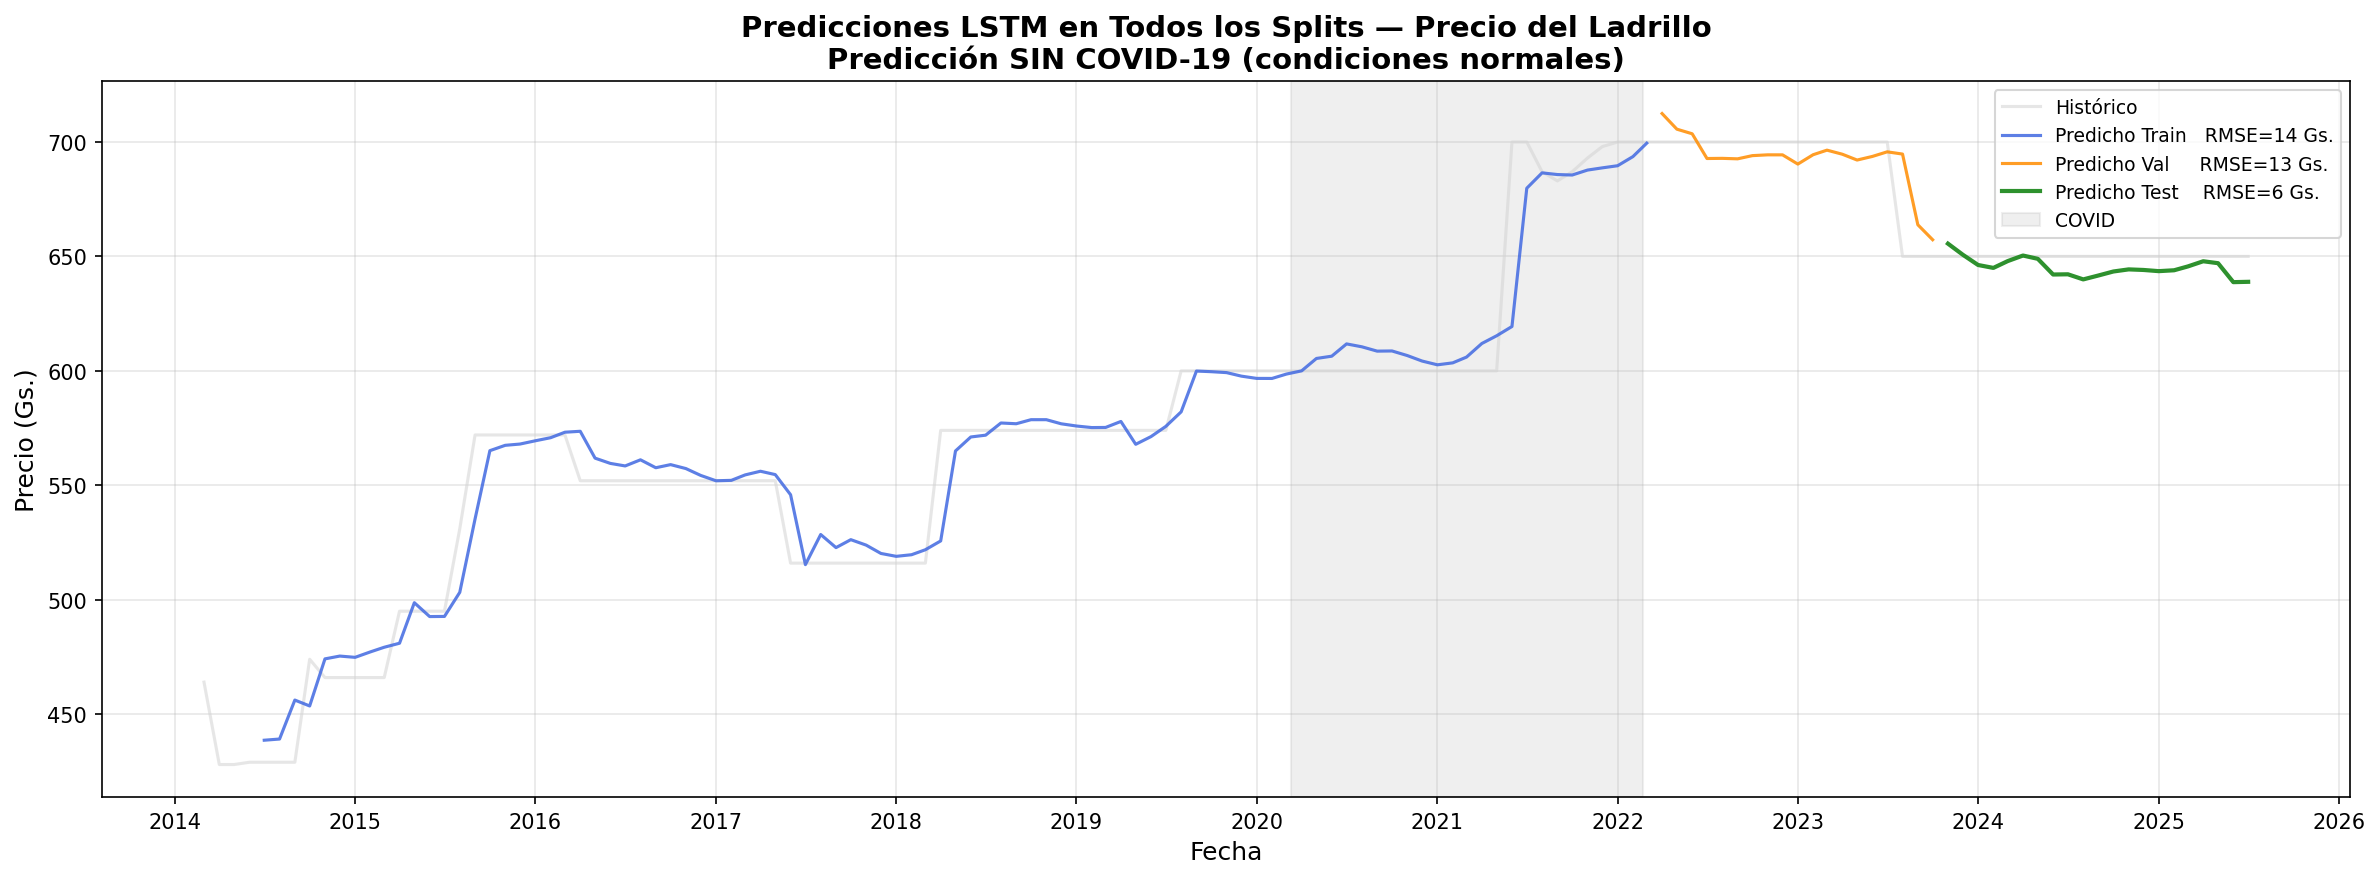
\includegraphics[width=\textwidth]{predicciones/prediccion_ladrillo_lstm/resultados_sin_covid/final_05_todos_splits.png}
    \caption{Ajuste del modelo LSTM del ladrillo sobre las tres particiones --- escenario sin pandemia.}
    \label{fig:lstm_ladrillo_splits_sc}
\end{figure}

\clearpage
\paragraph{Análisis de Residuos}

\begin{figure}[htbp]
    \centering
    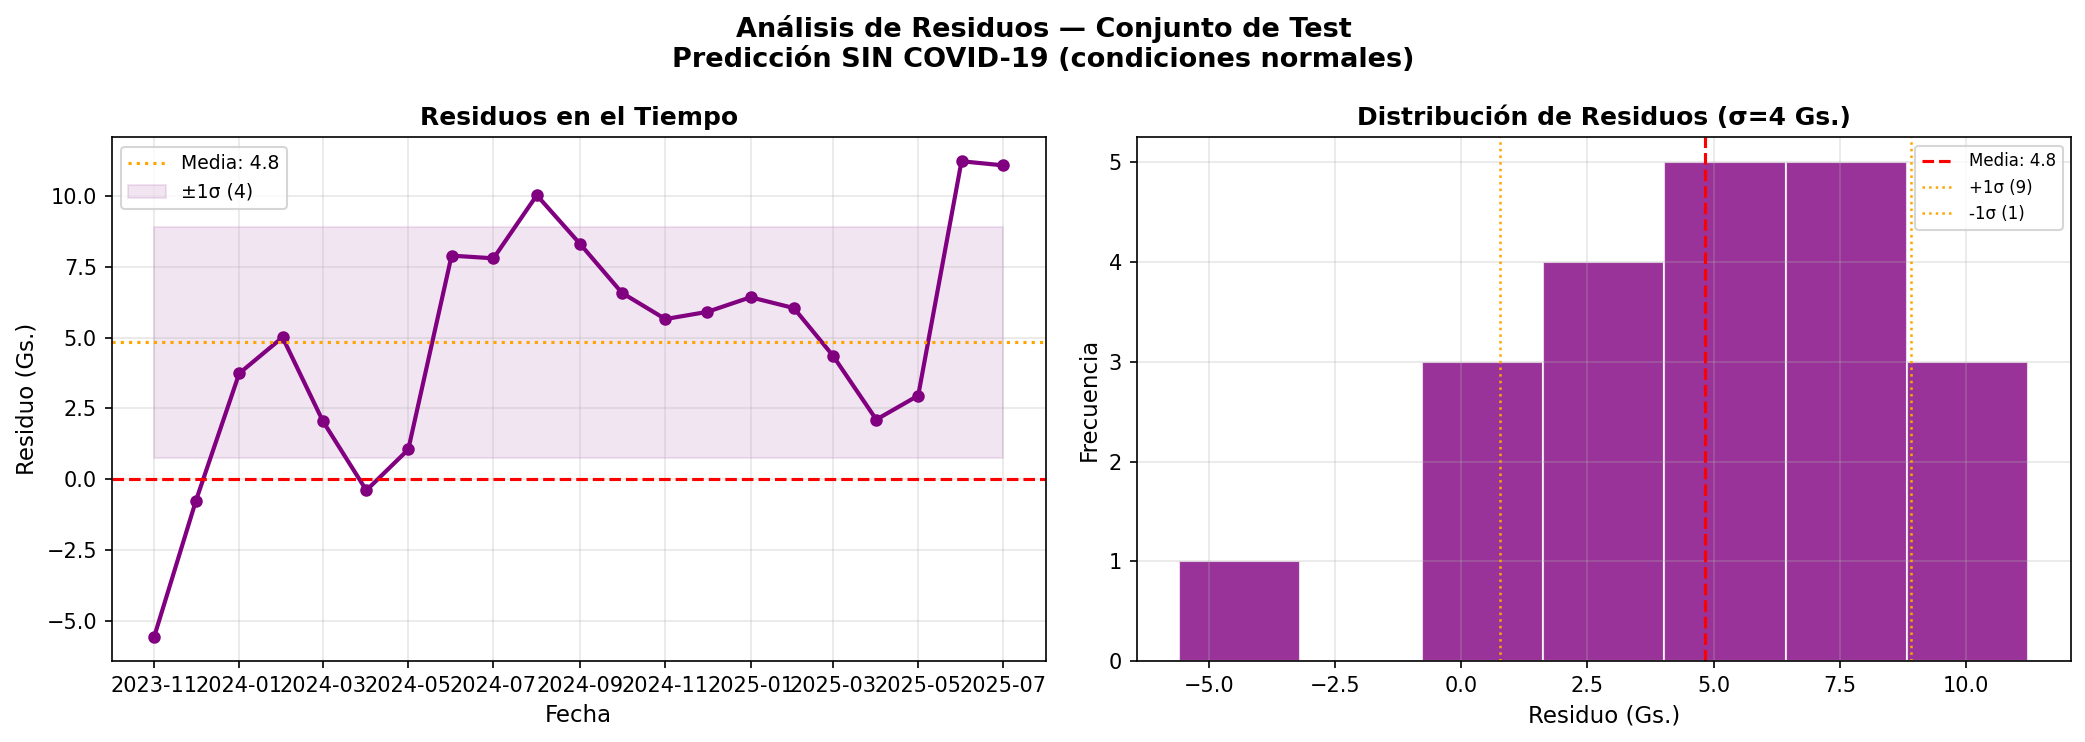
\includegraphics[width=\textwidth]{predicciones/prediccion_ladrillo_lstm/resultados_sin_covid/final_04_residuos.png}
    \caption{Residuos del modelo LSTM para ladrillo sobre el conjunto de prueba --- escenario sin pandemia.}
    \label{fig:lstm_ladrillo_res_sc}
\end{figure}

\begin{figure}[htbp]
    \centering
    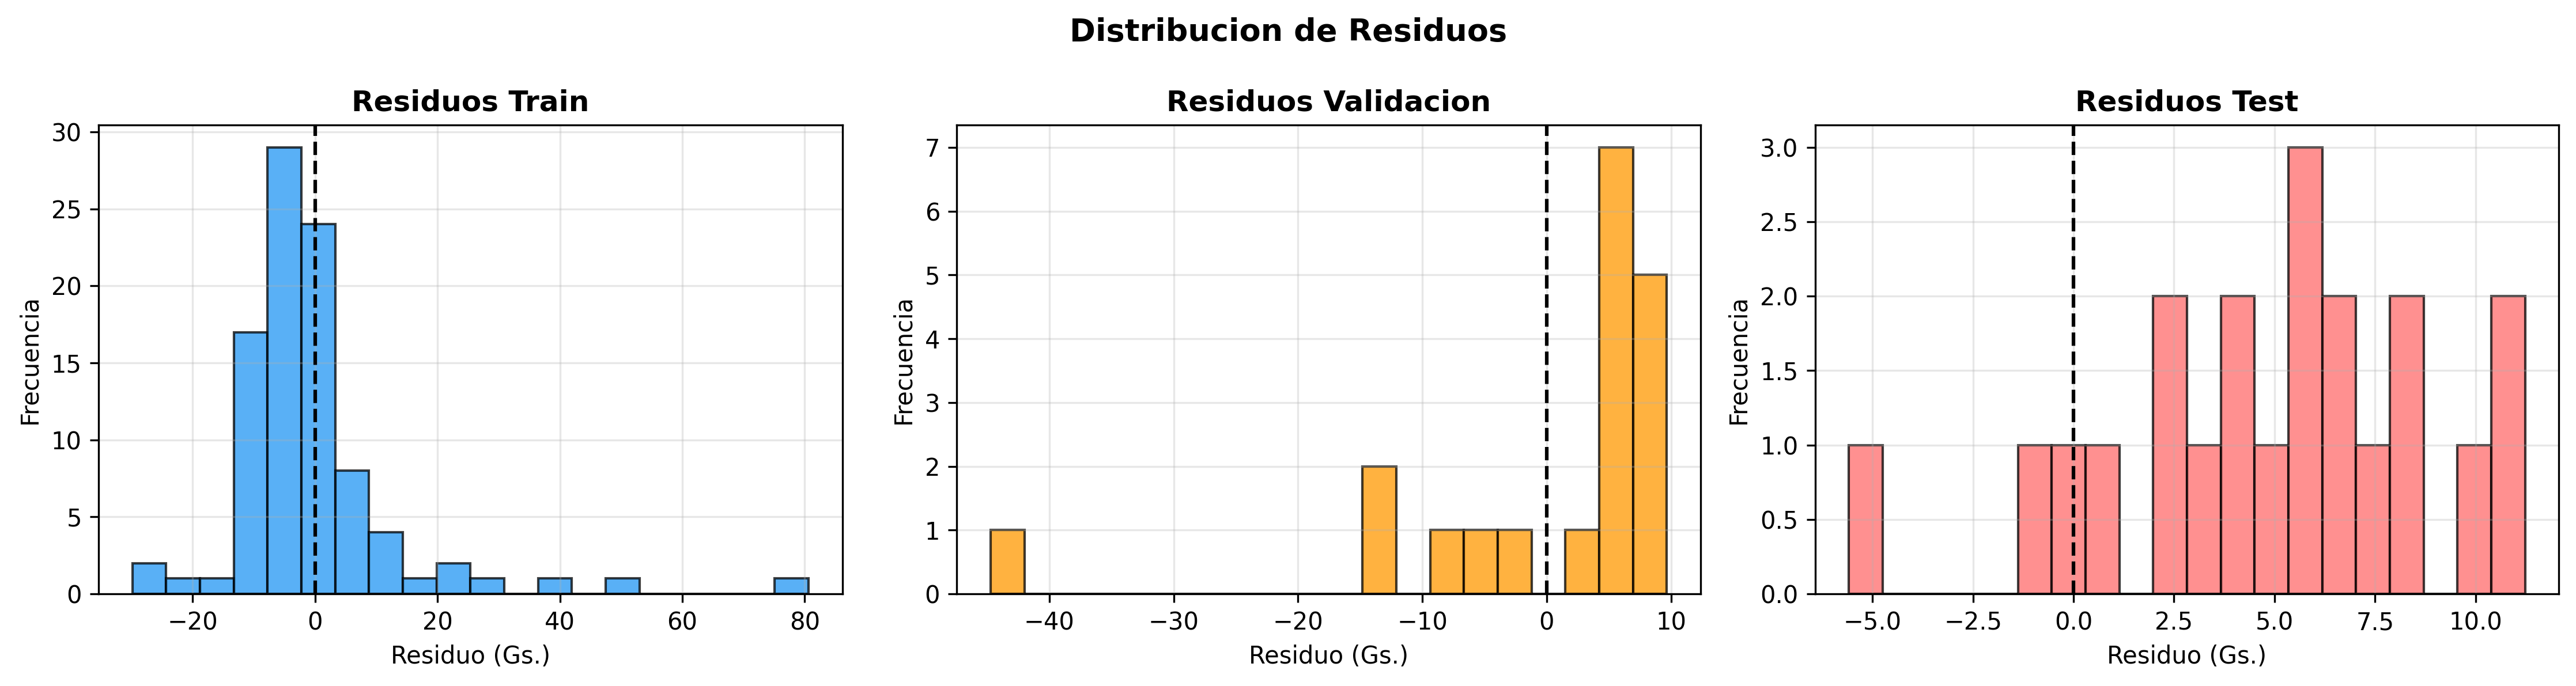
\includegraphics[width=0.75\textwidth]{predicciones/prediccion_ladrillo_lstm/resultados_sin_covid/residuos_histograma.png}
    \caption{Histograma de residuos del modelo LSTM para ladrillo --- escenario sin pandemia.}
    \label{fig:lstm_ladrillo_reshist_sc}
\end{figure}

\begin{figure}[htbp]
    \centering
    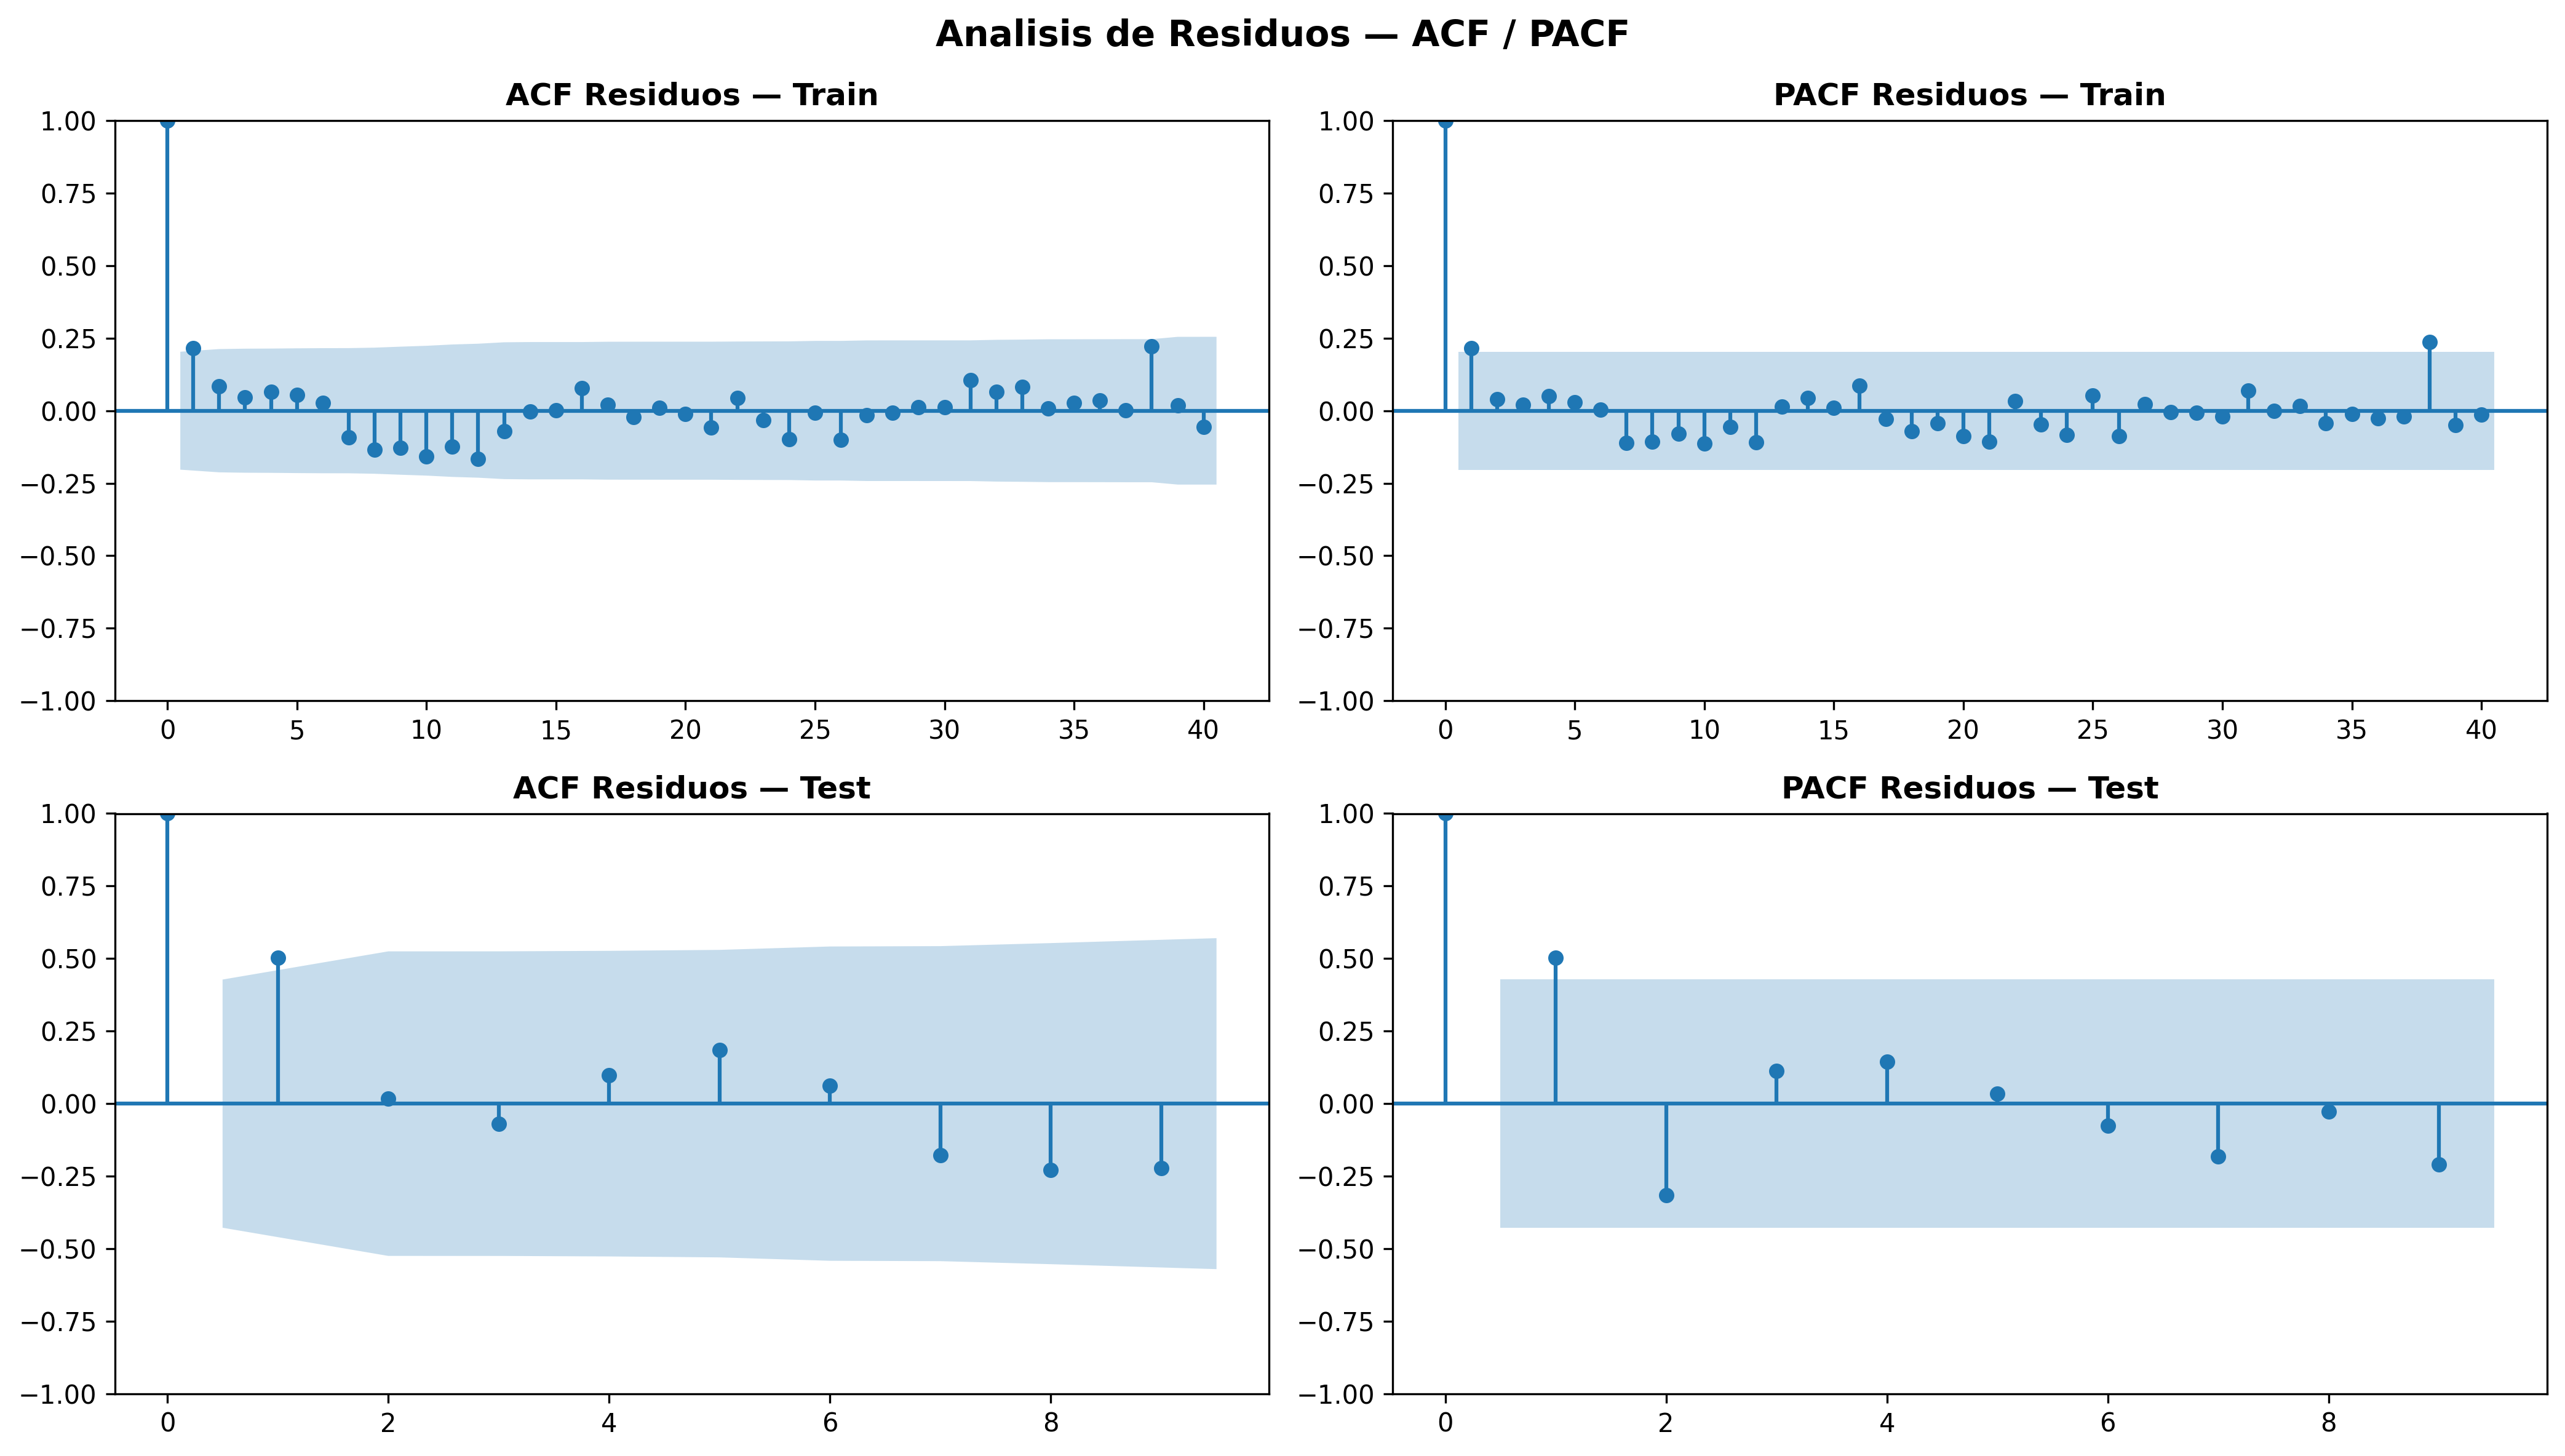
\includegraphics[width=\textwidth]{predicciones/prediccion_ladrillo_lstm/resultados_sin_covid/residuos_acf_pacf.png}
    \caption{ACF y PACF de los residuos del modelo LSTM para ladrillo --- escenario sin pandemia.}
    \label{fig:lstm_ladrillo_resacf_sc}
\end{figure}

\justify
El test de Ljung-Box sobre los residuos del conjunto de prueba muestra un $p$-valor de 0,237 a 10 rezagos (no rechaza $H_0$) y un $p$-valor de $1{,}05 \times 10^{-5}$ a 20 rezagos (rechaza $H_0$). Esto indica que los residuos se comportan como ruido blanco en el corto plazo, aunque existen patrones de dependencia en rezagos más distantes, posiblemente asociados a estacionalidad no capturada completamente.

\clearpage
\paragraph{Pronóstico a 24 Meses}

\begin{figure}[htbp]
    \centering
    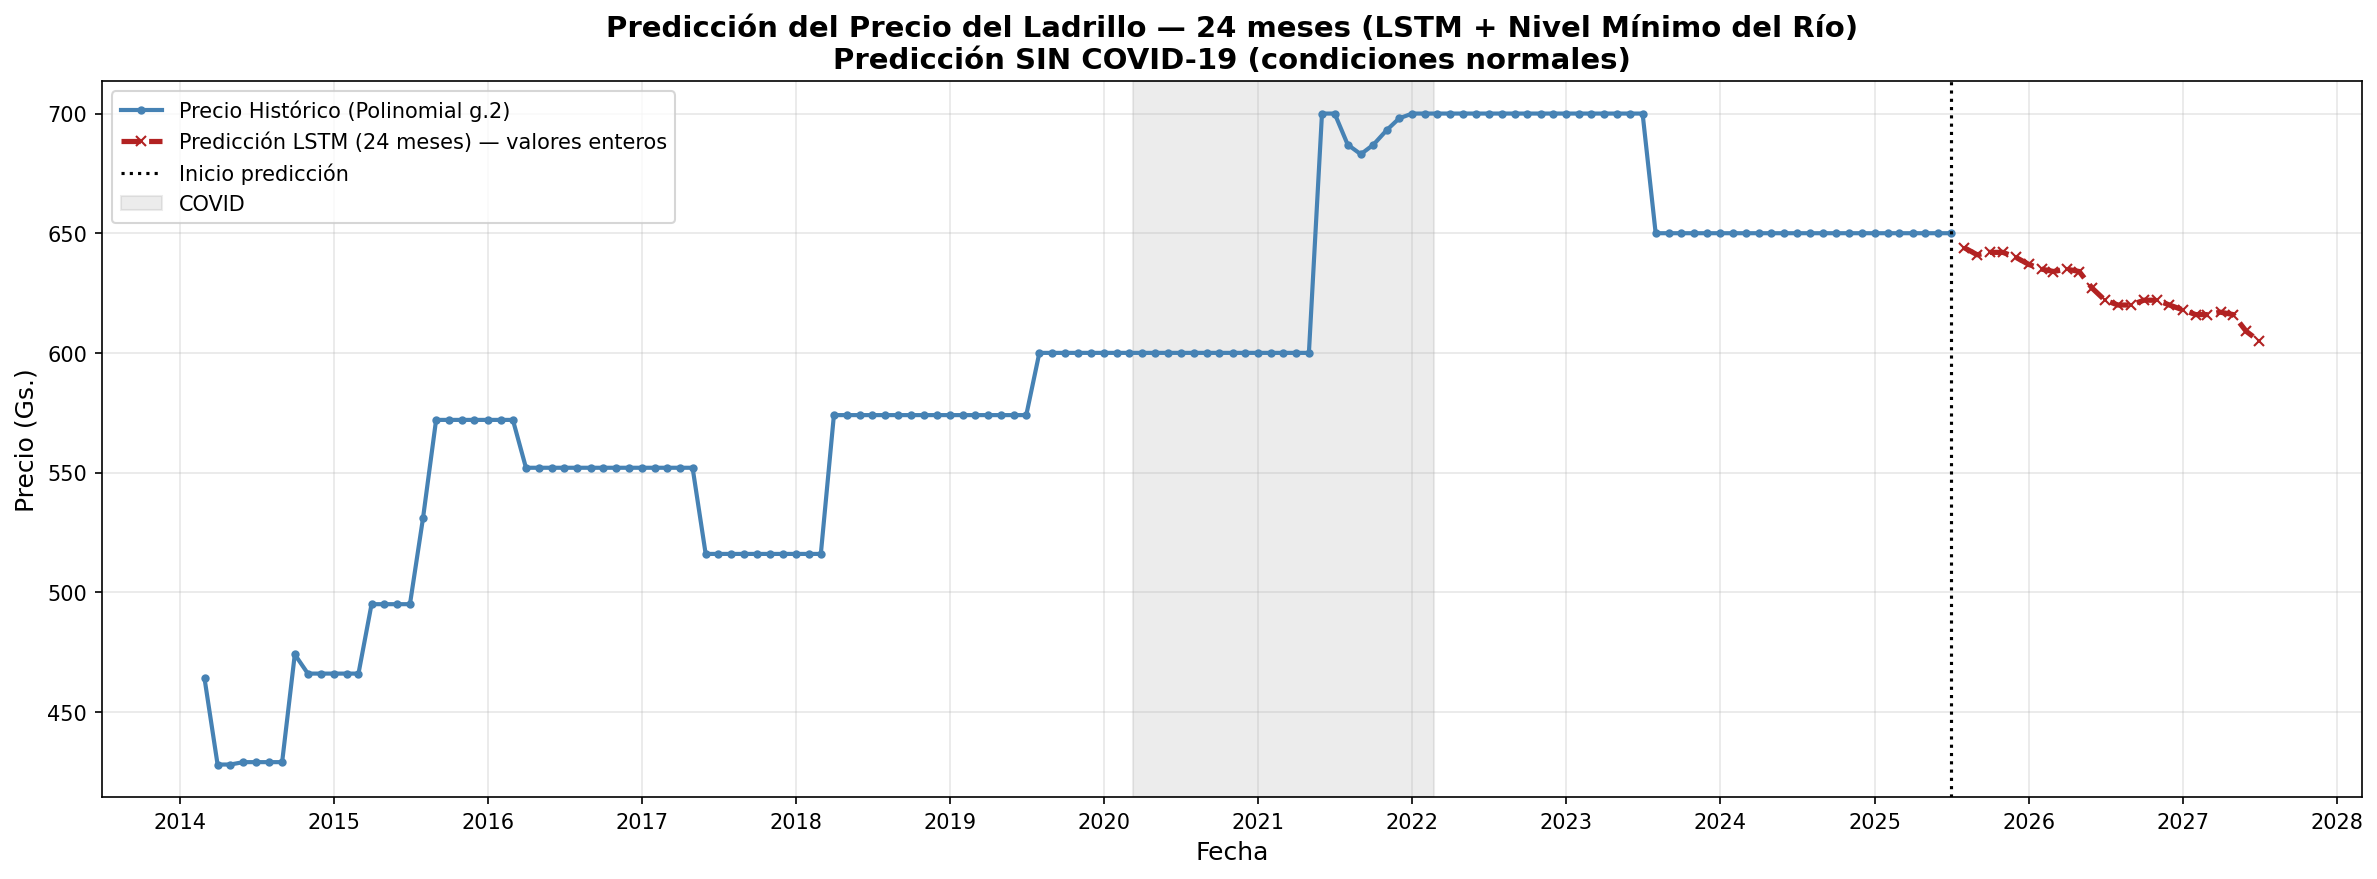
\includegraphics[width=\textwidth]{predicciones/prediccion_ladrillo_lstm/resultados_sin_covid/final_06_prediccion_futura_completa.png}
    \caption{Pronóstico LSTM a 24 meses del precio del ladrillo --- escenario sin pandemia, con IC al 95\,\%.}
    \label{fig:lstm_ladrillo_pred_sin_covid}
\end{figure}

\begin{figure}[htbp]
    \centering
    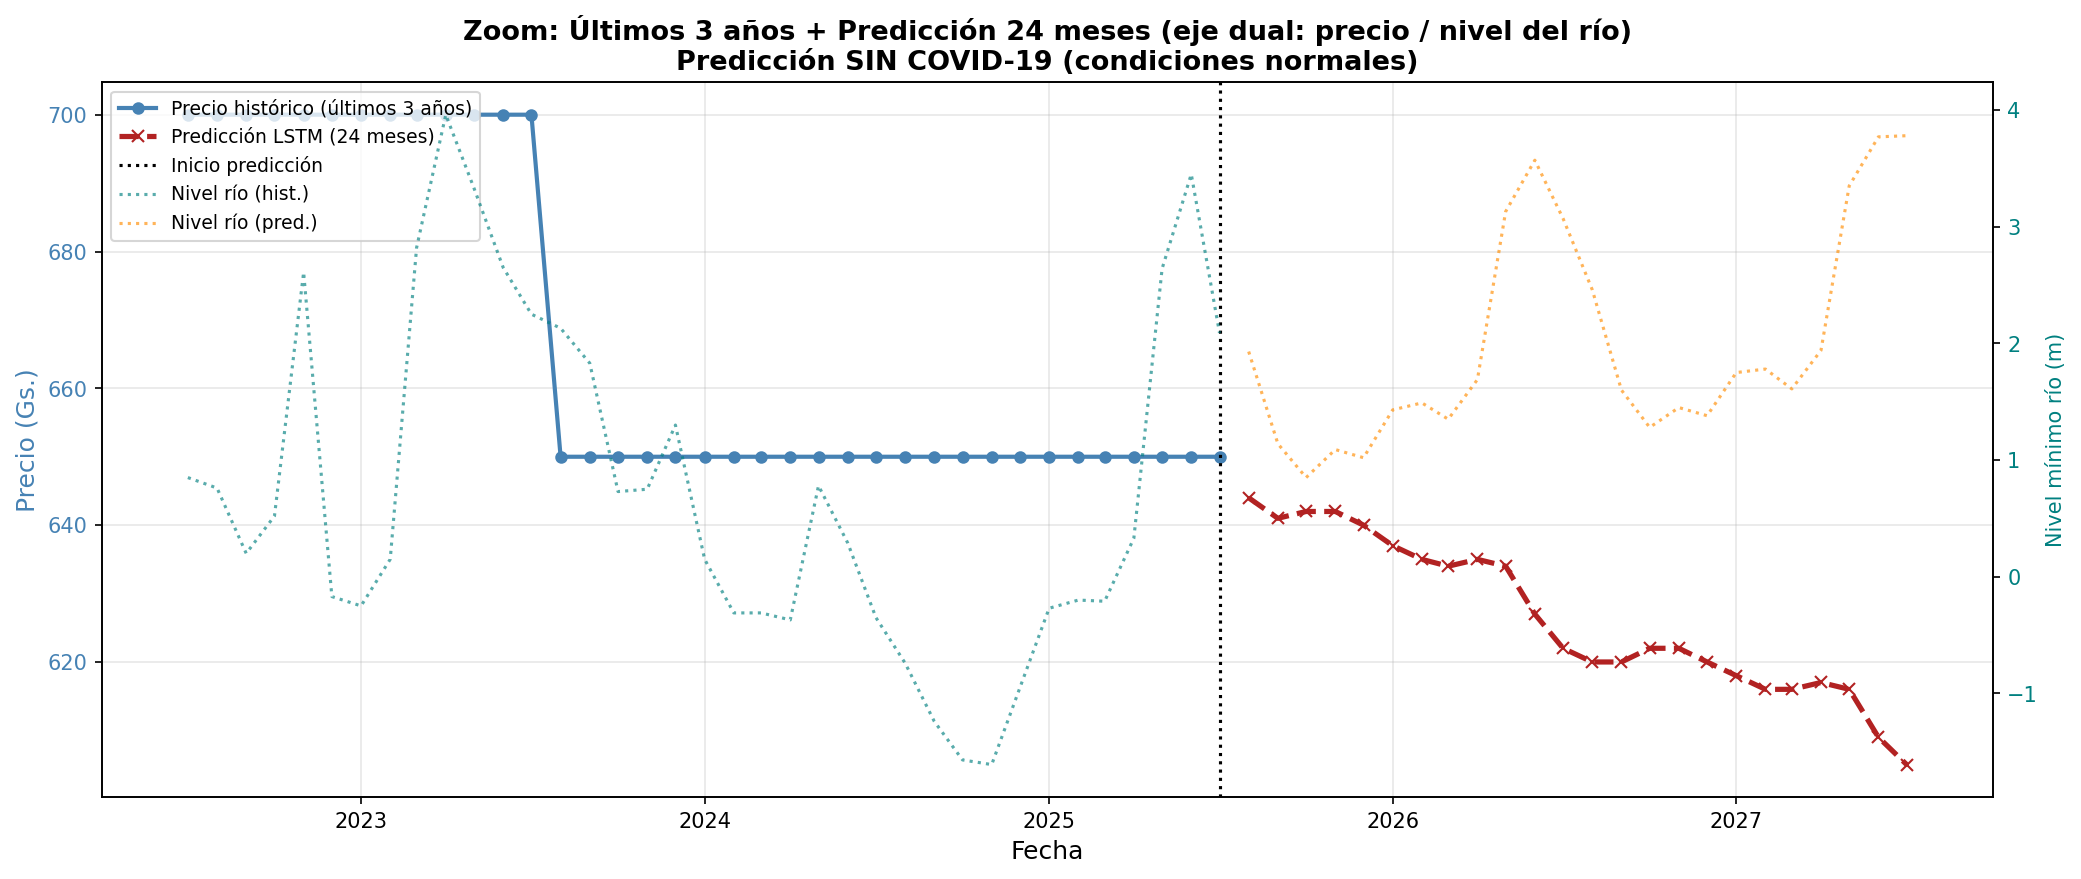
\includegraphics[width=\textwidth]{predicciones/prediccion_ladrillo_lstm/resultados_sin_covid/final_07_prediccion_zoom_dual.png}
    \caption{Detalle de la transición histórico--pronóstico LSTM del ladrillo --- escenario sin pandemia.}
    \label{fig:lstm_ladrillo_zoom_sin_covid}
\end{figure}

\begin{figure}[htbp]
    \centering
    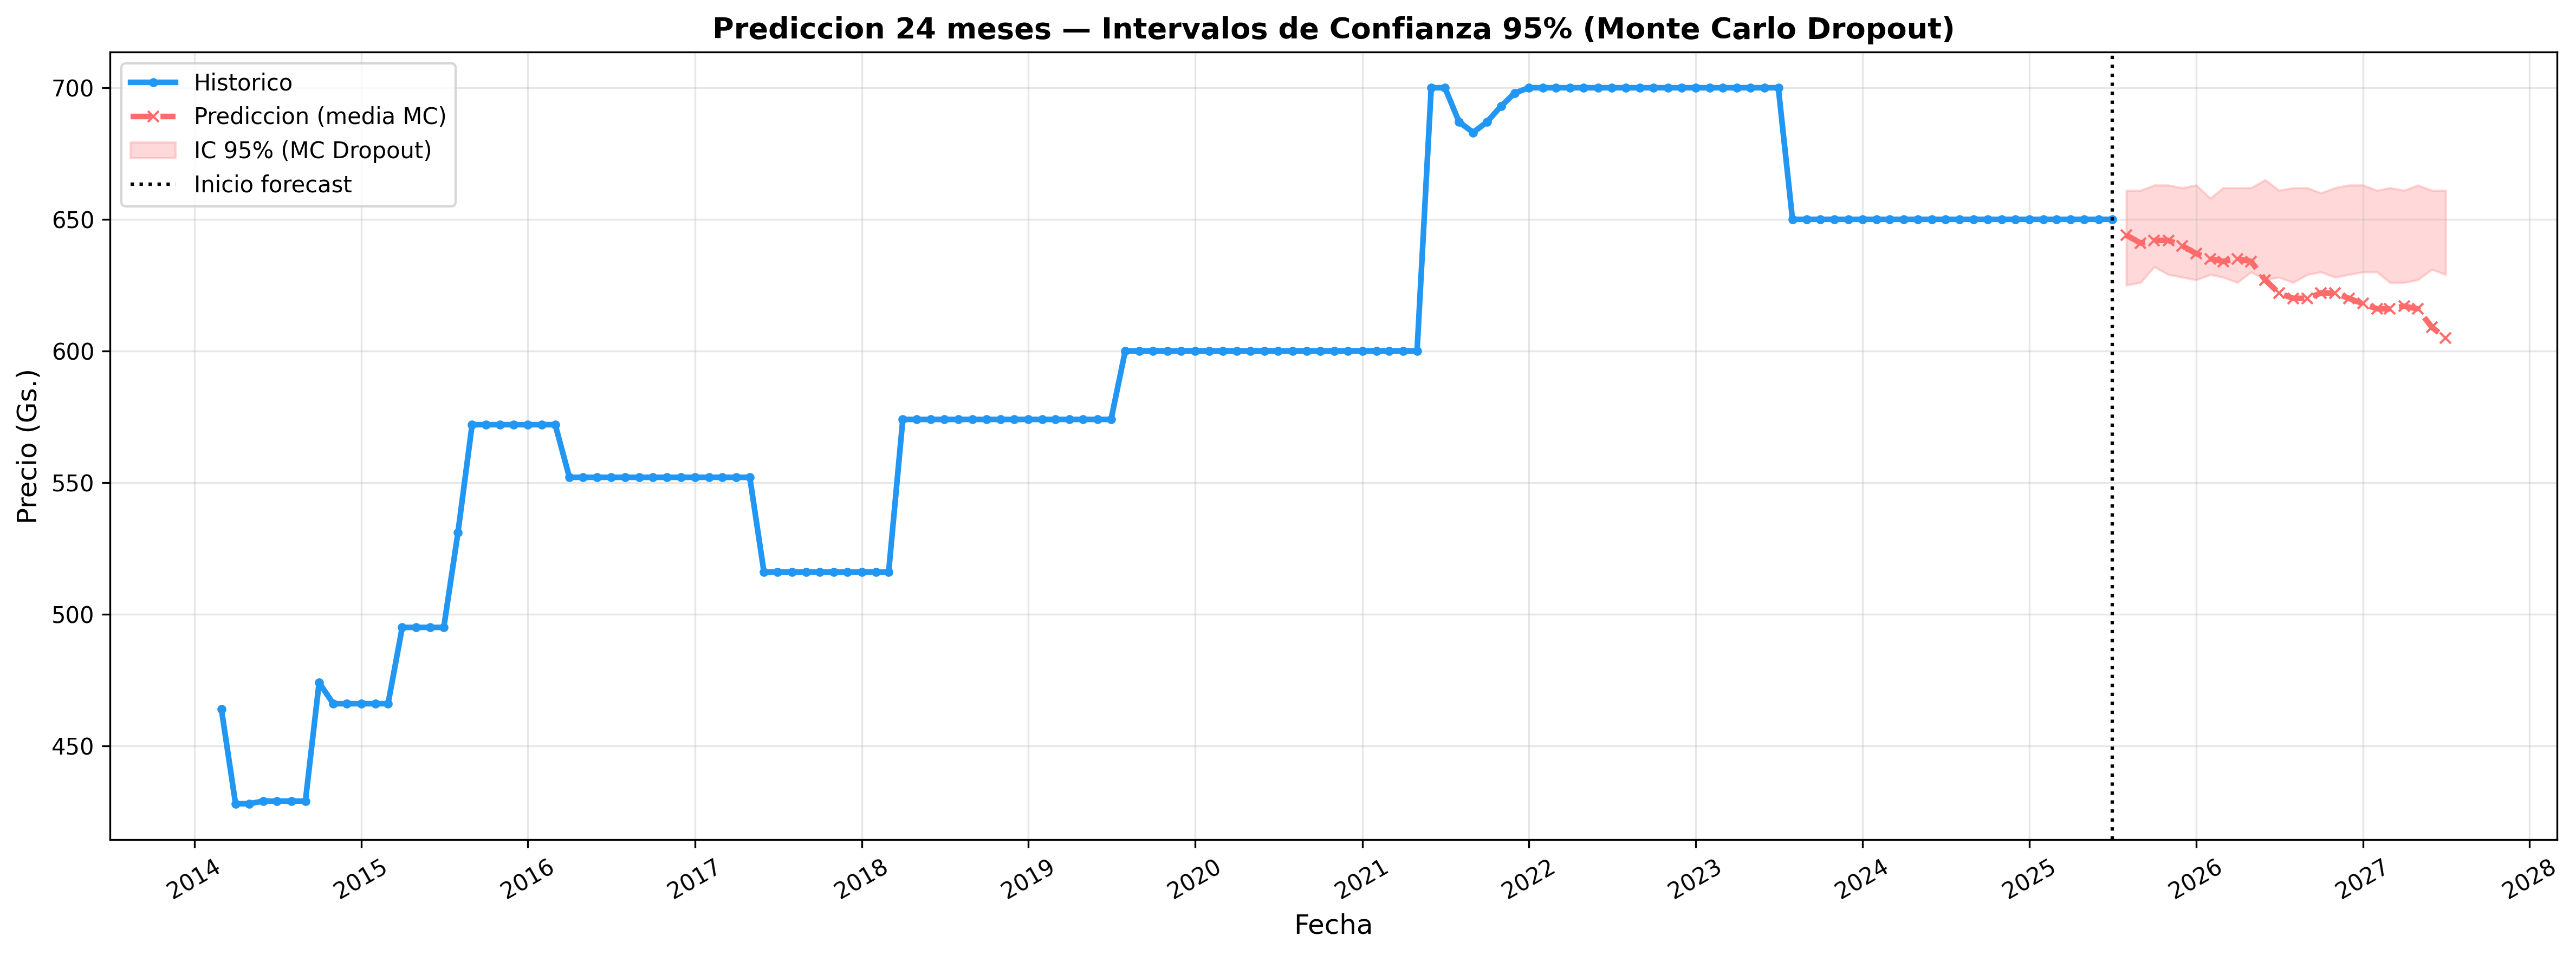
\includegraphics[width=\textwidth]{predicciones/prediccion_ladrillo_lstm/resultados_sin_covid/forecast_ic_monte_carlo.png}
    \caption{IC Monte Carlo Dropout del pronóstico LSTM para ladrillo --- escenario sin pandemia.}
    \label{fig:lstm_ladrillo_ic_mc_sin_covid}
\end{figure}

\justify
Bajo el escenario sin pandemia, el rango de precios predicho se sitúa entre Gs.~605 y Gs.~644 a lo largo del horizonte de 24 meses, un rango estrecho que refleja la estabilidad relativa del precio del ladrillo en condiciones normales de mercado.

% ------ LADRILLO CON COVID ------
\clearpage
\subsubsection{Escenario con Efecto Pandémico}

\paragraph{Hiperparámetros y Arquitectura}

\justify
Para el escenario con efecto pandémico, la búsqueda con Optuna convergió a una arquitectura diferente: una capa LSTM \textbf{unidireccional} con 64 unidades ocultas, sin \textit{dropout} ni planificador de tasa de aprendizaje. El optimizador fue Adam con $\text{lr}=0{,}001$, regularización L2 $\lambda=10^{-5}$, \textit{lookback} de 6 meses y \textit{batch size} de 4. La Tabla~\ref{tab:lstm_ladrillo_cc_hiper} detalla estos parámetros.

\begin{table}[htbp]
\centering
\caption{Hiperparámetros del modelo LSTM para ladrillo --- escenario con pandemia.}
\label{tab:lstm_ladrillo_cc_hiper}
\begin{tabular}{ll}
\toprule
\textbf{Hiperparámetro} & \textbf{Valor} \\
\midrule
Capas LSTM          & 1 \\
Unidades ocultas    & 64 \\
Bidireccional       & No \\
Dropout             & 0,0 \\
Dropout recurrente  & 0,0 \\
Optimizador         & Adam \\
Tasa de aprendizaje & 0,001 \\
Regularización L2   & $10^{-5}$ \\
Lookback            & 6 meses \\
Batch size          & 4 \\
Scheduler           & Ninguno \\
Parámetros entrenables & 18.497 \\
\bottomrule
\end{tabular}
\end{table}

\paragraph{Curva de Aprendizaje}

\begin{figure}[htbp]
    \centering
    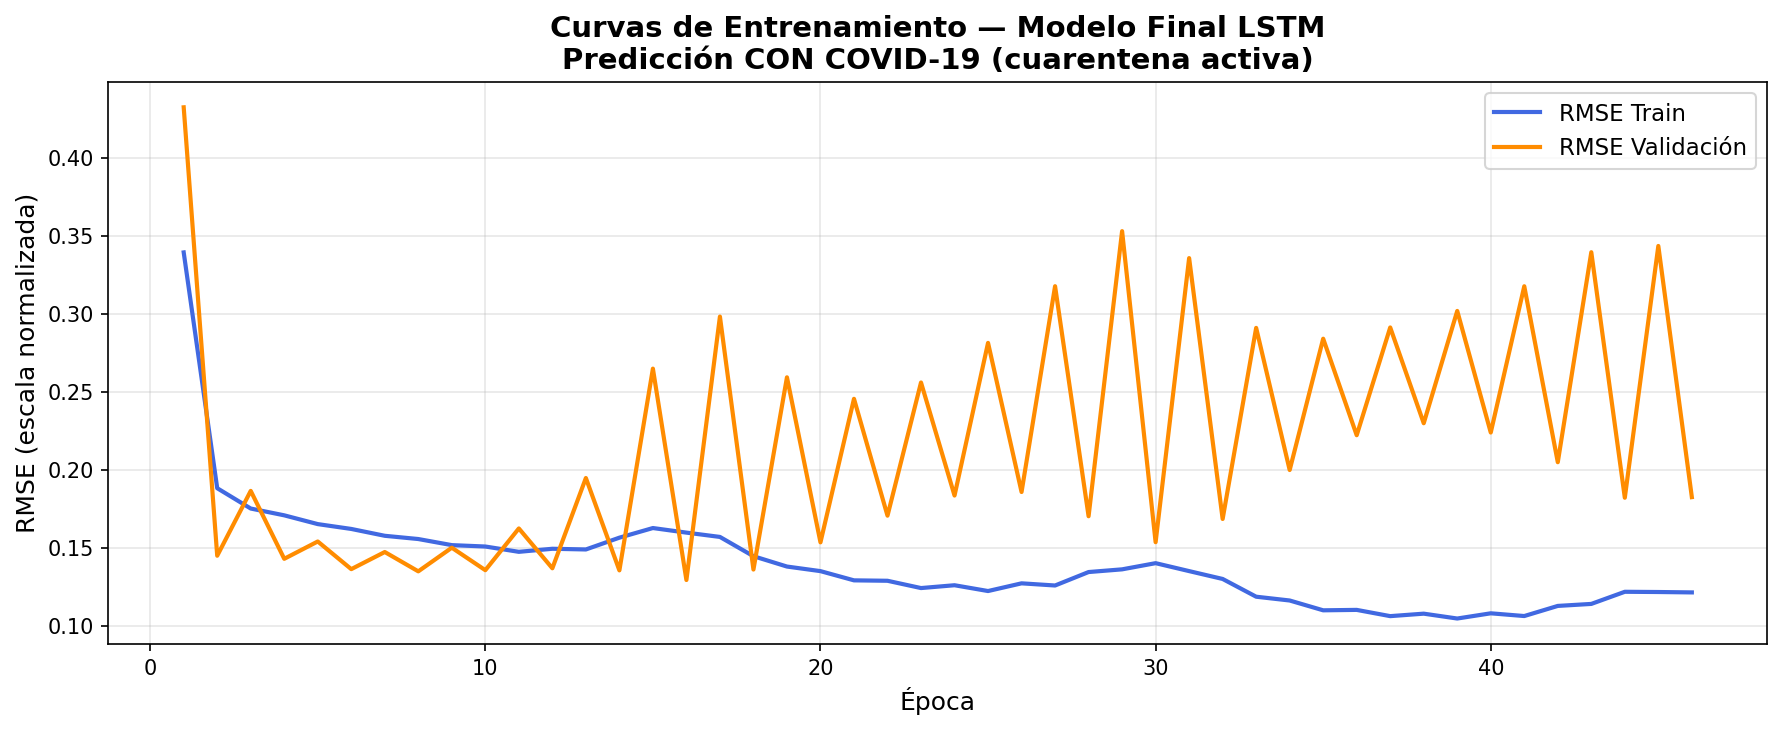
\includegraphics[width=0.85\textwidth]{predicciones/prediccion_ladrillo_lstm/resultados_con_covid/final_01_curvas_entrenamiento.png}
    \caption{Curva de aprendizaje del modelo LSTM para ladrillo --- escenario con pandemia.}
    \label{fig:lstm_ladrillo_curva_cc}
\end{figure}

\paragraph{Métricas de Evaluación}

\begin{table}[htbp]
\centering
\caption{Desempeño del modelo LSTM para ladrillo --- escenario con pandemia: RMSE en train, val y test.}
\label{tab:lstm_ladrillo_cc_metricas}
\begin{tabular}{lrrr}
\toprule
\textbf{Métrica} & \textbf{Train} & \textbf{Val} & \textbf{Test} \\
\midrule
RMSE (Gs.) & 18,59 & 17,54 & 9,13 \\
\bottomrule
\end{tabular}
\end{table}

\justify
El RMSE de prueba de 9,13~Gs.\ es superior al obtenido en el escenario sin pandemia (6,32~Gs.), lo que refleja que la arquitectura unidireccional más simple ---con el efecto pandémico incluido en el entrenamiento--- no logra el mismo nivel de ajuste que el modelo bidireccional optimizado para el escenario sin pandemia. No obstante, representa un error relativo inferior al 3\,\% del rango histórico de la serie, que sigue siendo aceptable para la predicción de precios de materiales de construcción.

\paragraph{Evaluación sobre el Conjunto de Prueba}

\begin{figure}[htbp]
    \centering
    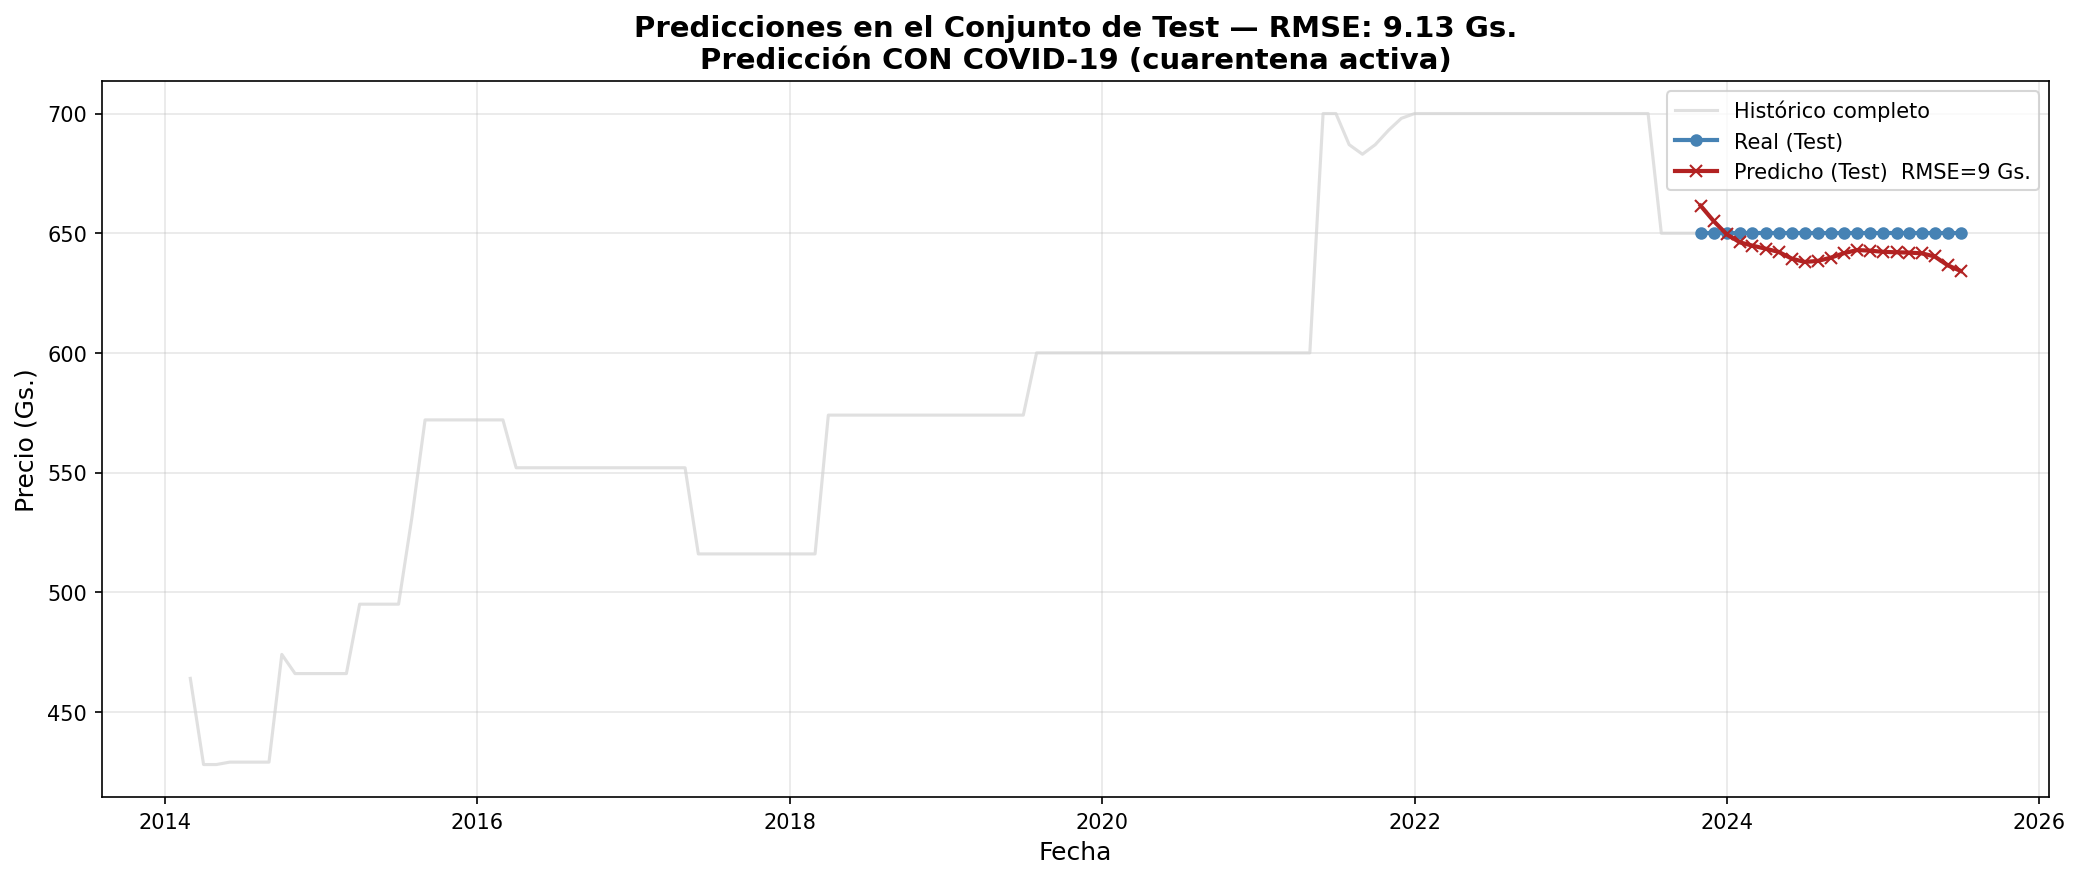
\includegraphics[width=\textwidth]{predicciones/prediccion_ladrillo_lstm/resultados_con_covid/final_02_prediccion_test_serie.png}
    \caption{Predicción LSTM vs.\ valores reales del precio del ladrillo --- escenario con pandemia, conjunto de prueba.}
    \label{fig:lstm_ladrillo_test_cc}
\end{figure}

\begin{figure}[htbp]
    \centering
    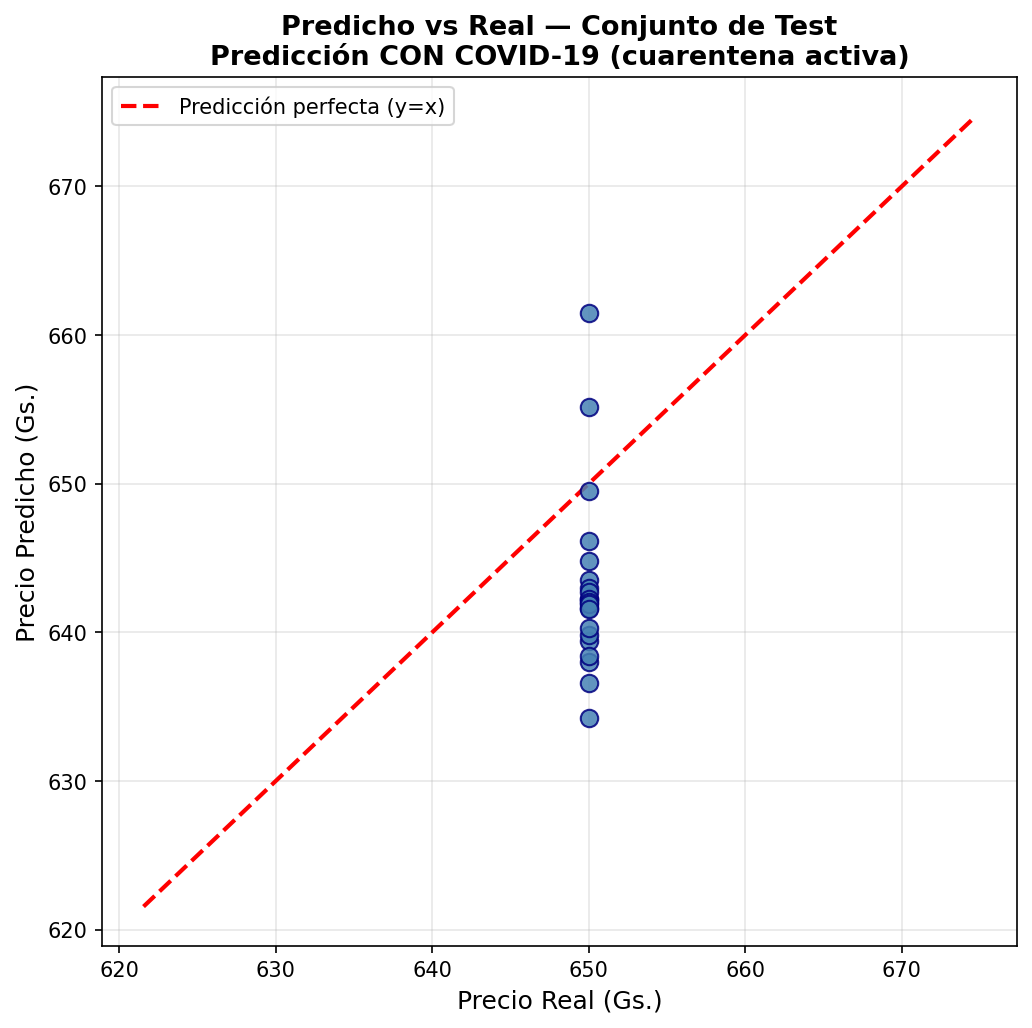
\includegraphics[width=0.7\textwidth]{predicciones/prediccion_ladrillo_lstm/resultados_con_covid/final_03_scatter_test.png}
    \caption{Diagrama de dispersión: precio predicho vs.\ real del ladrillo --- escenario con pandemia.}
    \label{fig:lstm_ladrillo_scatter_cc}
\end{figure}

\begin{figure}[htbp]
    \centering
    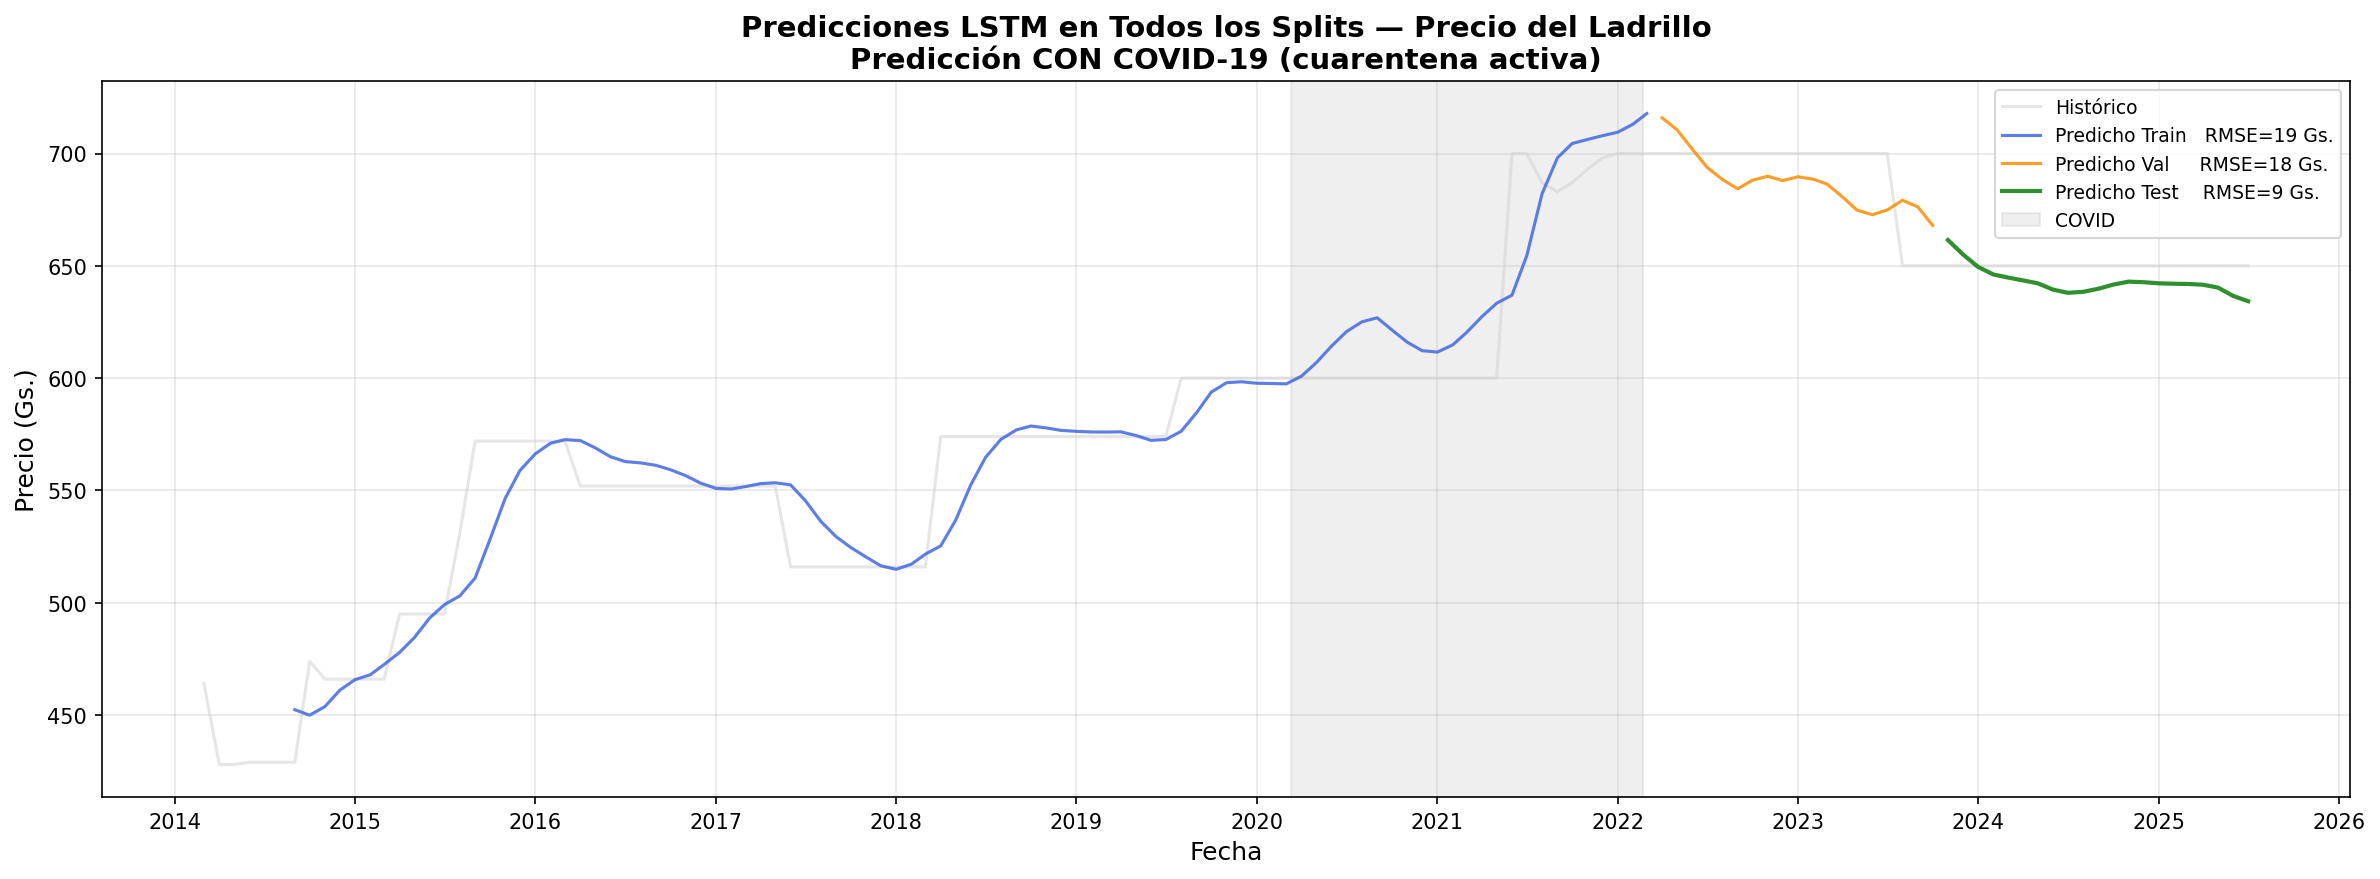
\includegraphics[width=\textwidth]{predicciones/prediccion_ladrillo_lstm/resultados_con_covid/final_05_todos_splits.png}
    \caption{Ajuste del modelo LSTM del ladrillo sobre las tres particiones --- escenario con pandemia.}
    \label{fig:lstm_ladrillo_splits_cc}
\end{figure}

\clearpage
\paragraph{Análisis de Residuos}

\begin{figure}[htbp]
    \centering
    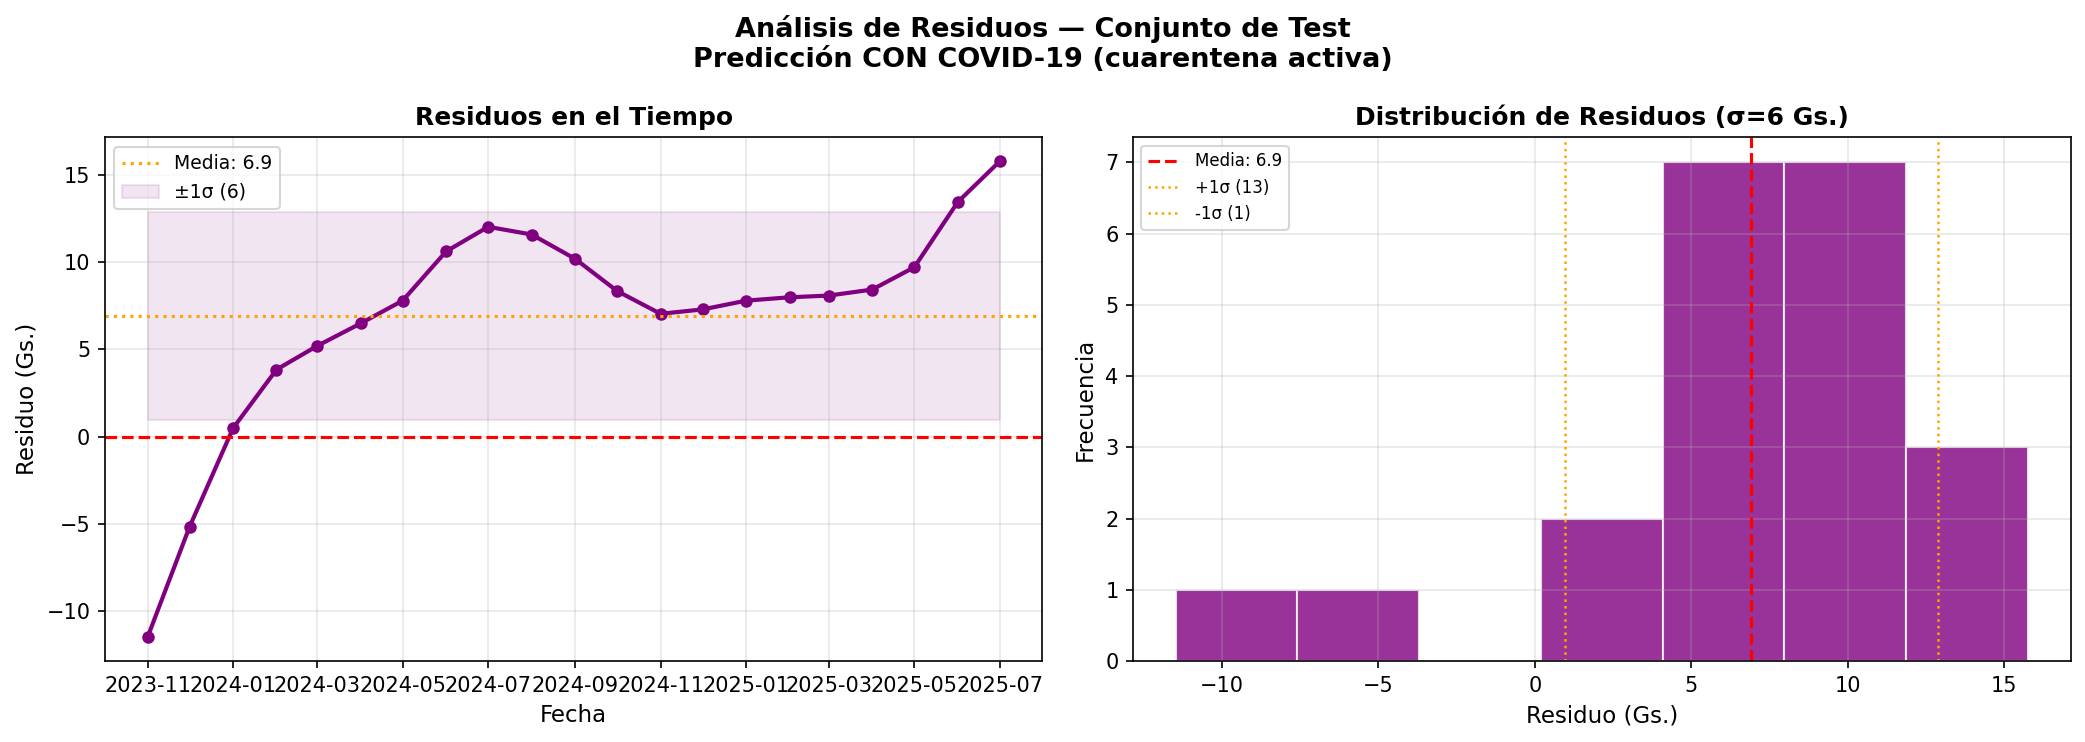
\includegraphics[width=\textwidth]{predicciones/prediccion_ladrillo_lstm/resultados_con_covid/final_04_residuos.png}
    \caption{Residuos del modelo LSTM para ladrillo sobre el conjunto de prueba --- escenario con pandemia.}
    \label{fig:lstm_ladrillo_res_cc}
\end{figure}

\begin{figure}[htbp]
    \centering
    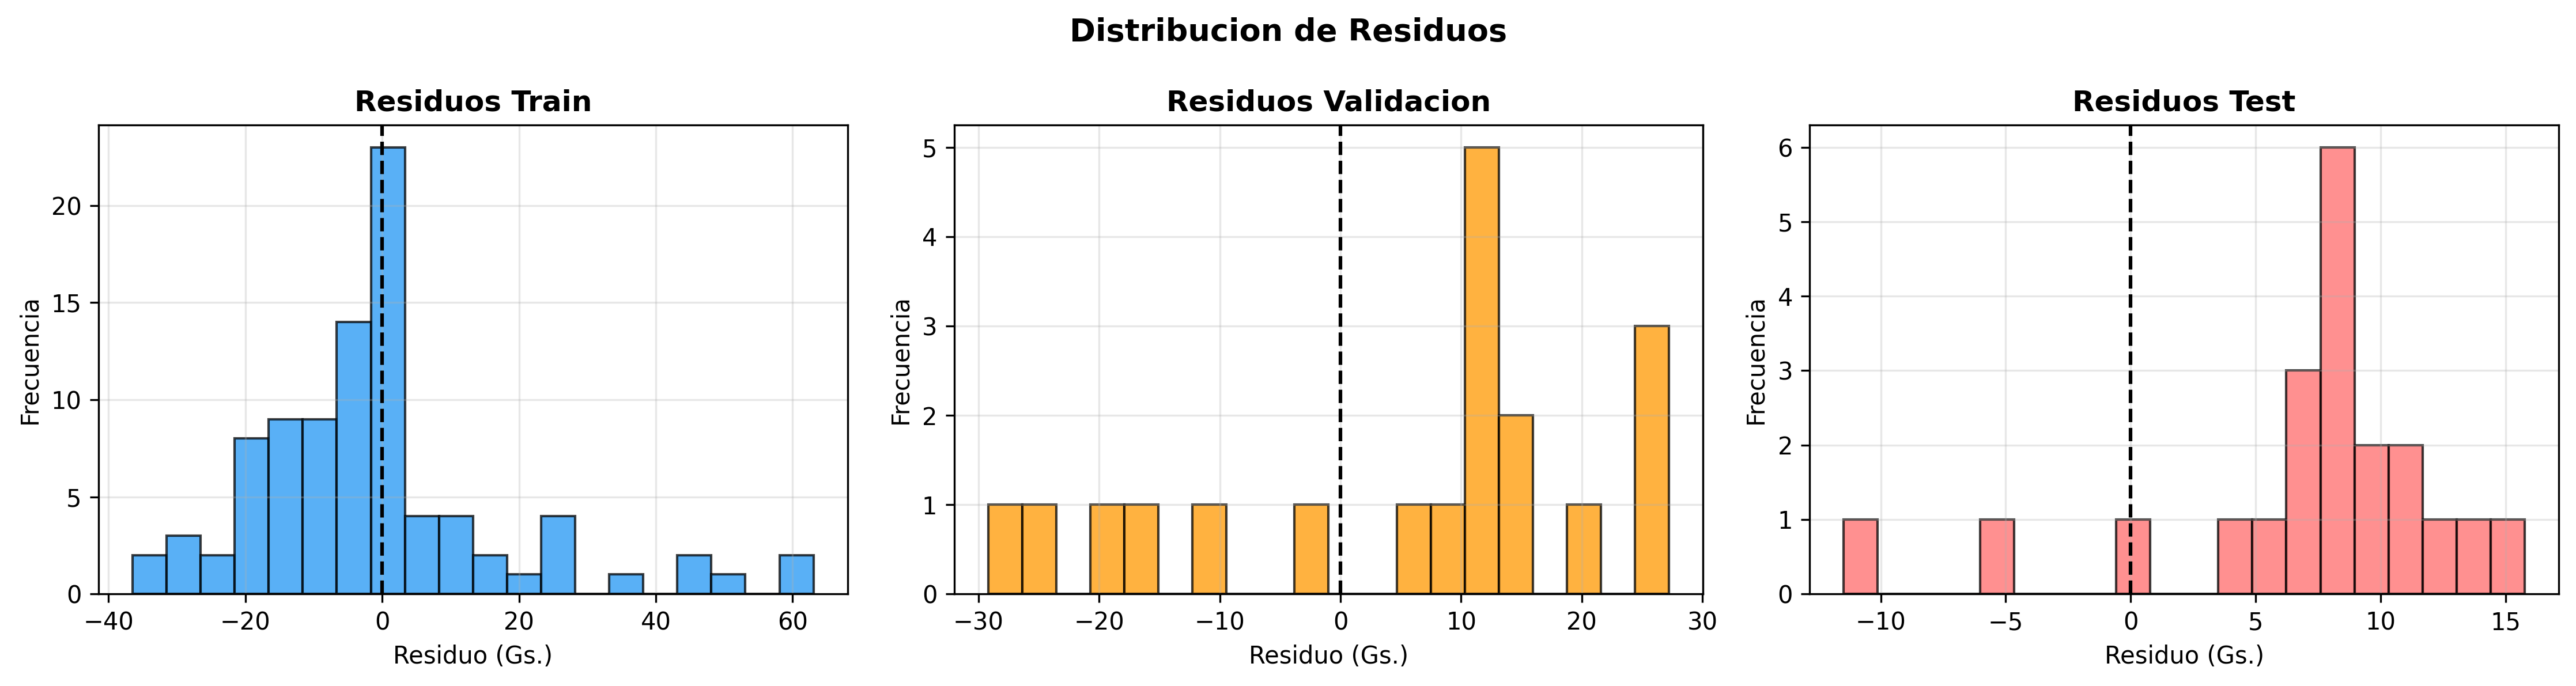
\includegraphics[width=0.75\textwidth]{predicciones/prediccion_ladrillo_lstm/resultados_con_covid/residuos_histograma.png}
    \caption{Histograma de residuos del modelo LSTM para ladrillo --- escenario con pandemia.}
    \label{fig:lstm_ladrillo_reshist_cc}
\end{figure}

\begin{figure}[htbp]
    \centering
    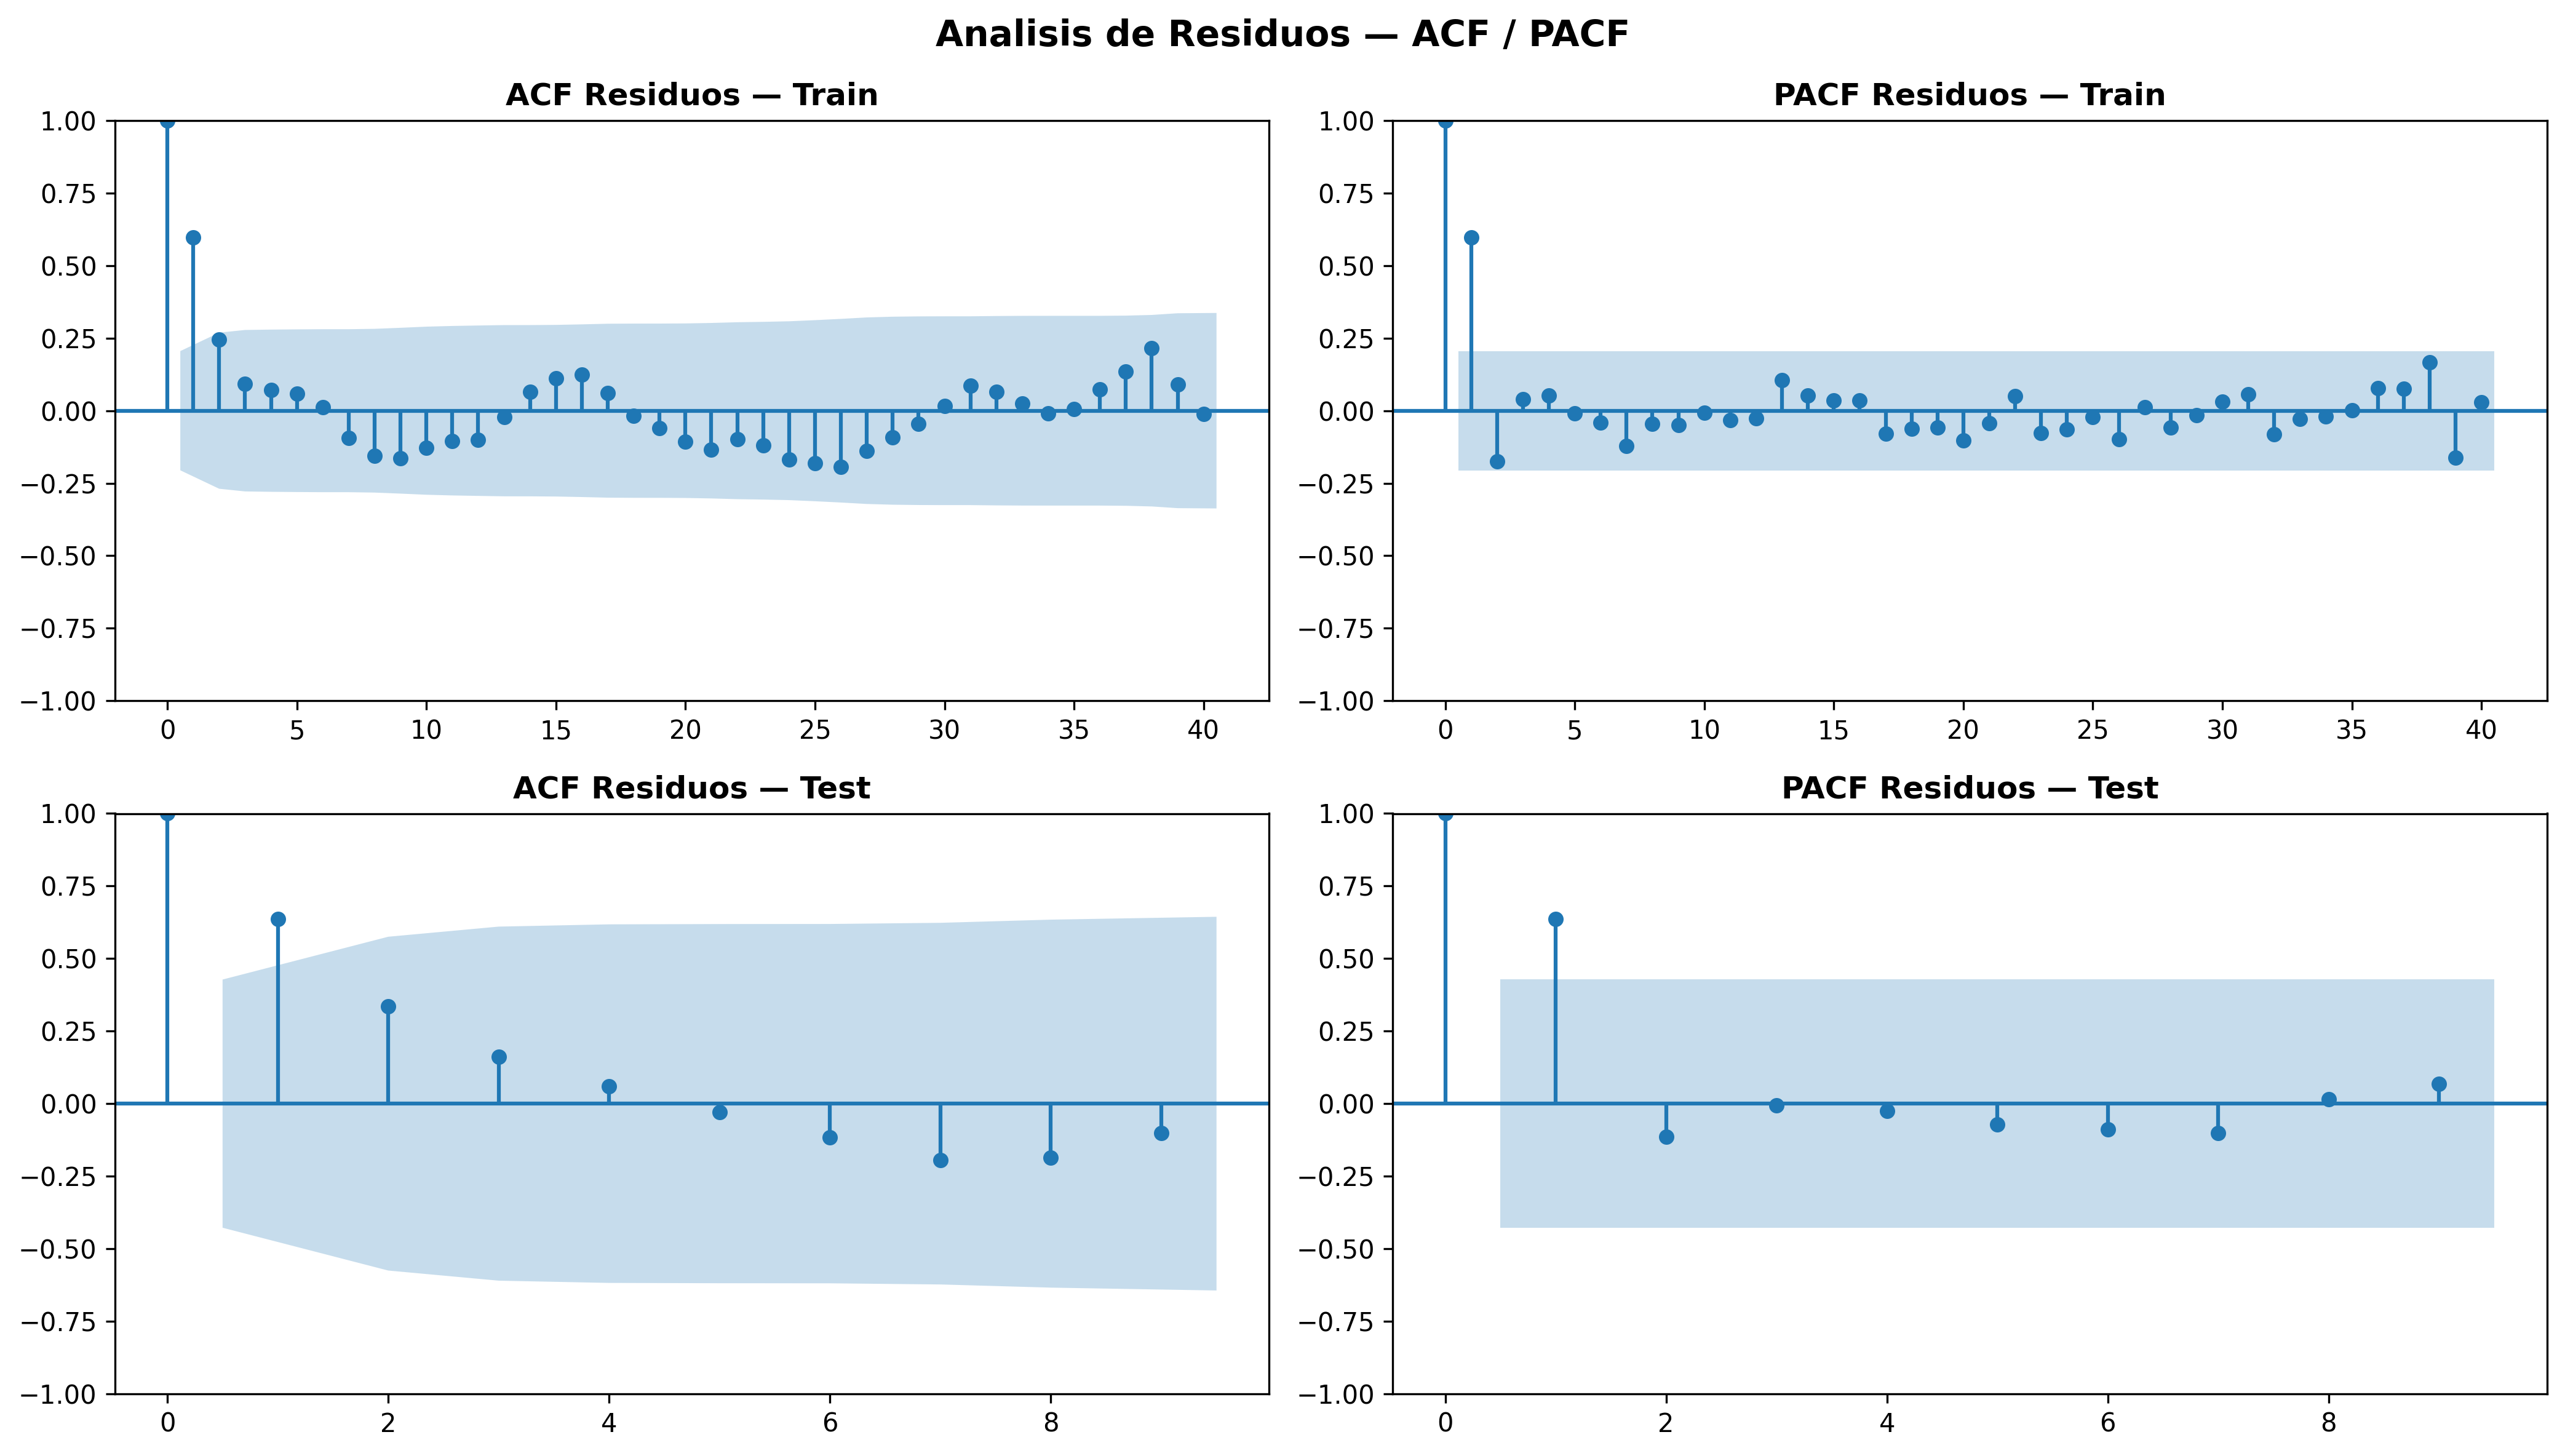
\includegraphics[width=\textwidth]{predicciones/prediccion_ladrillo_lstm/resultados_con_covid/residuos_acf_pacf.png}
    \caption{ACF y PACF de los residuos del modelo LSTM para ladrillo --- escenario con pandemia.}
    \label{fig:lstm_ladrillo_resacf_cc}
\end{figure}

\justify
El test de Ljung-Box sobre los residuos del conjunto de prueba muestra un $p$-valor de 0,077 a 10 rezagos (no rechaza $H_0$) y un $p$-valor de $6{,}70 \times 10^{-9}$ a 20 rezagos (rechaza fuertemente $H_0$). Al igual que en el escenario sin pandemia, los residuos se comportan como ruido blanco en los primeros rezagos pero muestran dependencia en rezagos más distantes.

\clearpage
\paragraph{Pronóstico a 24 Meses}

\begin{figure}[htbp]
    \centering
    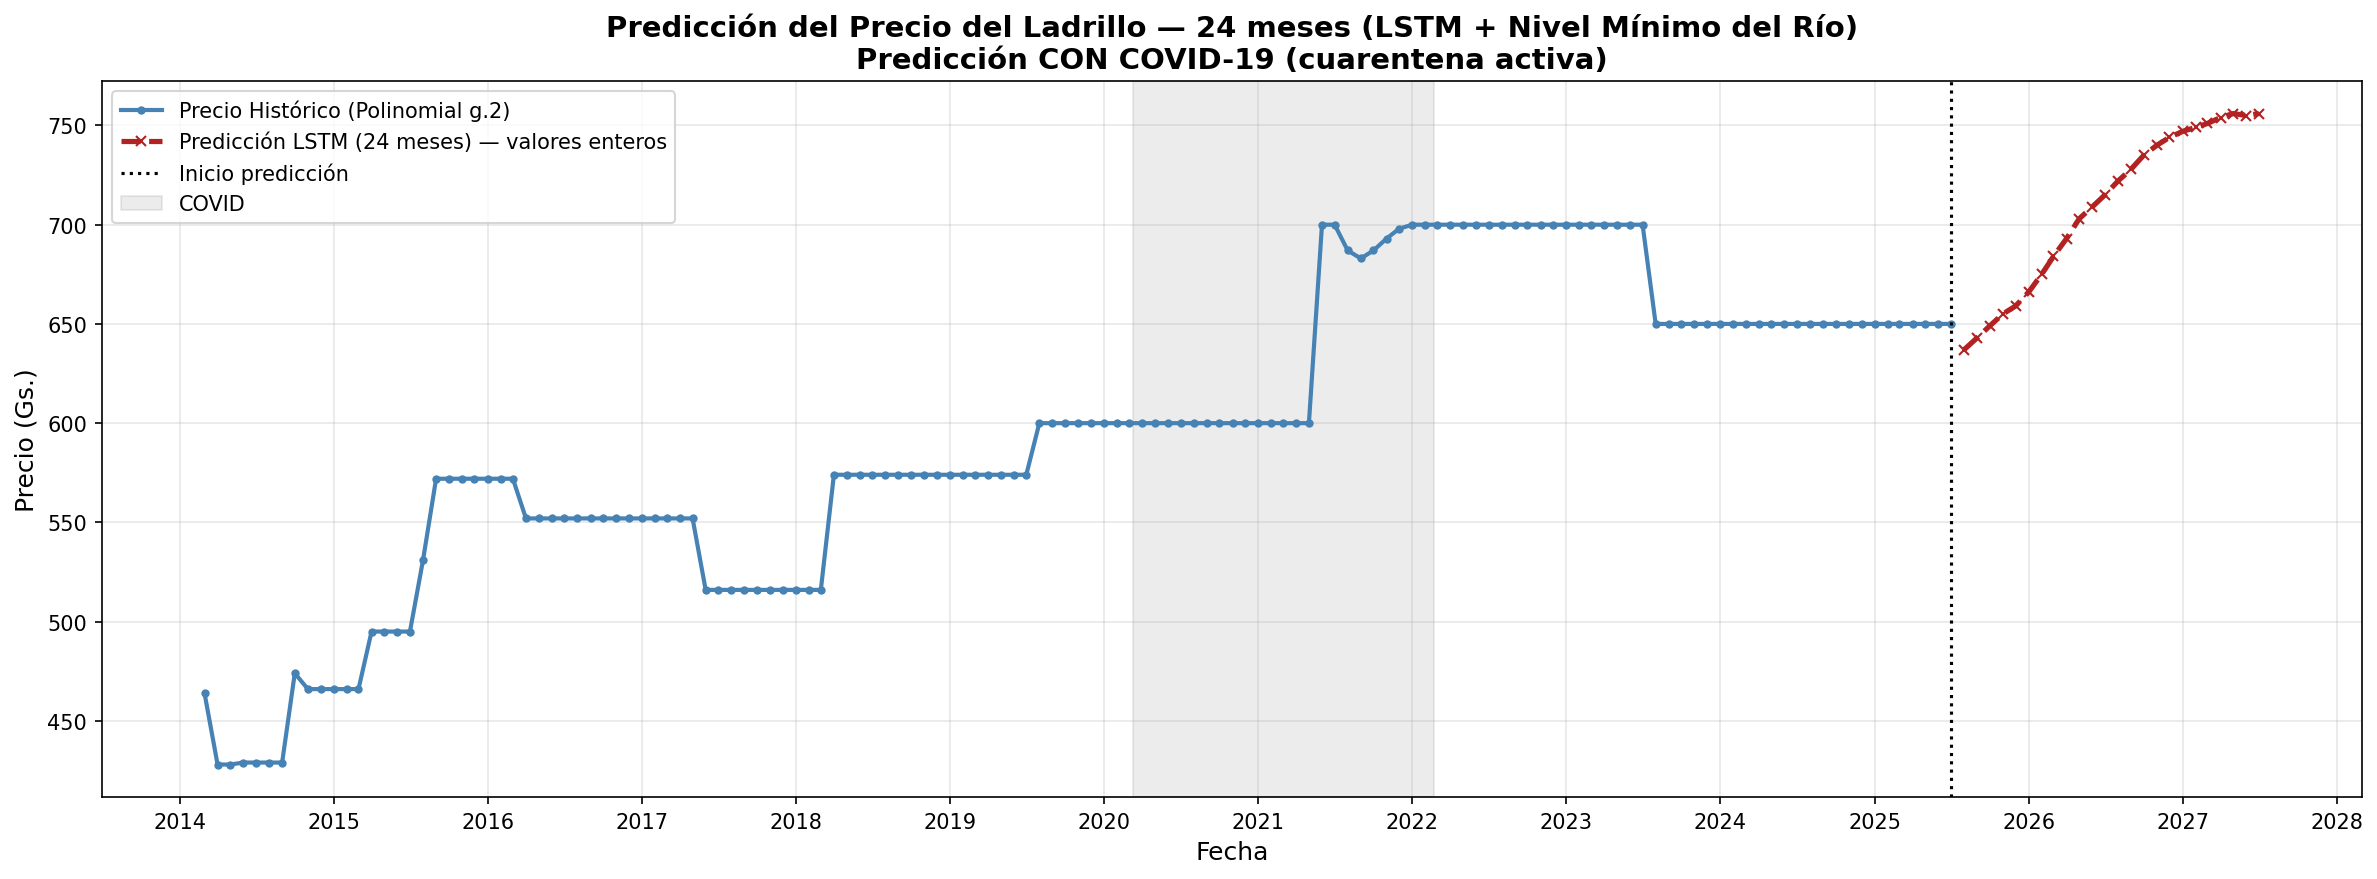
\includegraphics[width=\textwidth]{predicciones/prediccion_ladrillo_lstm/resultados_con_covid/final_06_prediccion_futura_completa.png}
    \caption{Pronóstico LSTM a 24 meses del precio del ladrillo --- escenario con pandemia, con IC al 95\,\%.}
    \label{fig:lstm_ladrillo_pred_con_covid}
\end{figure}

\begin{figure}[htbp]
    \centering
    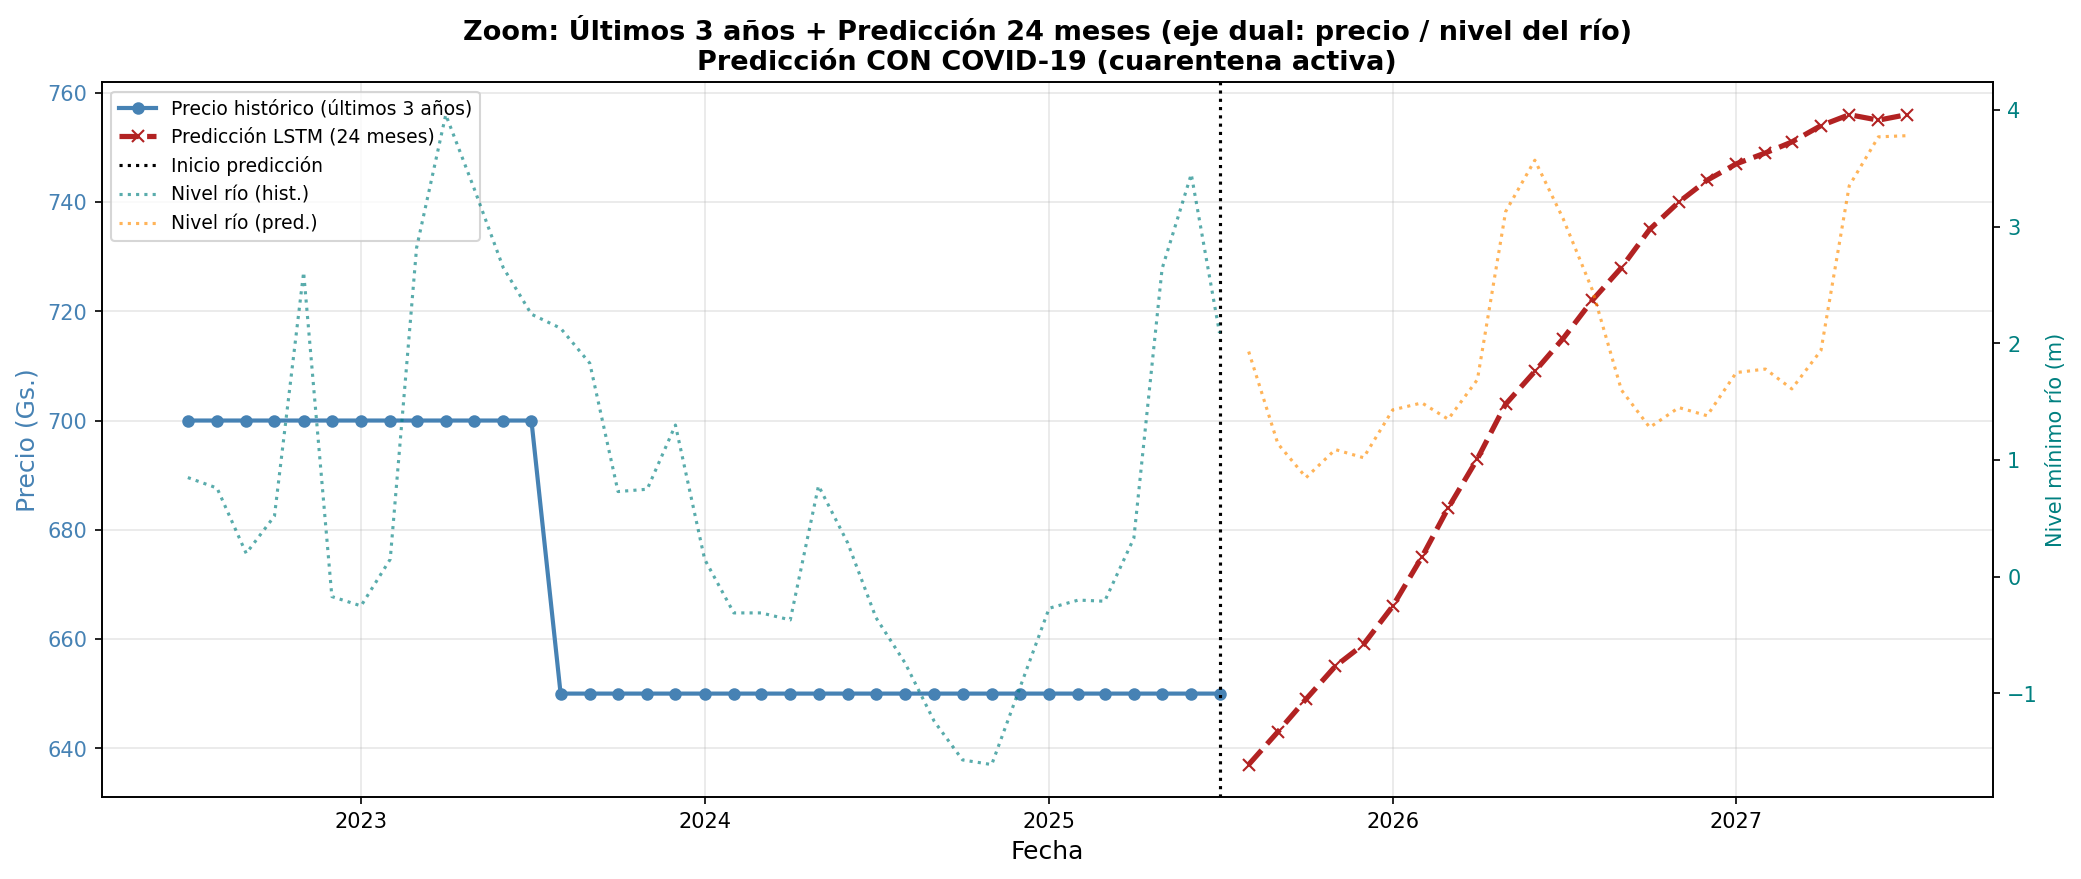
\includegraphics[width=\textwidth]{predicciones/prediccion_ladrillo_lstm/resultados_con_covid/final_07_prediccion_zoom_dual.png}
    \caption{Detalle de la transición histórico--pronóstico LSTM del ladrillo --- escenario con pandemia.}
    \label{fig:lstm_ladrillo_zoom_con_covid}
\end{figure}

\begin{figure}[htbp]
    \centering
    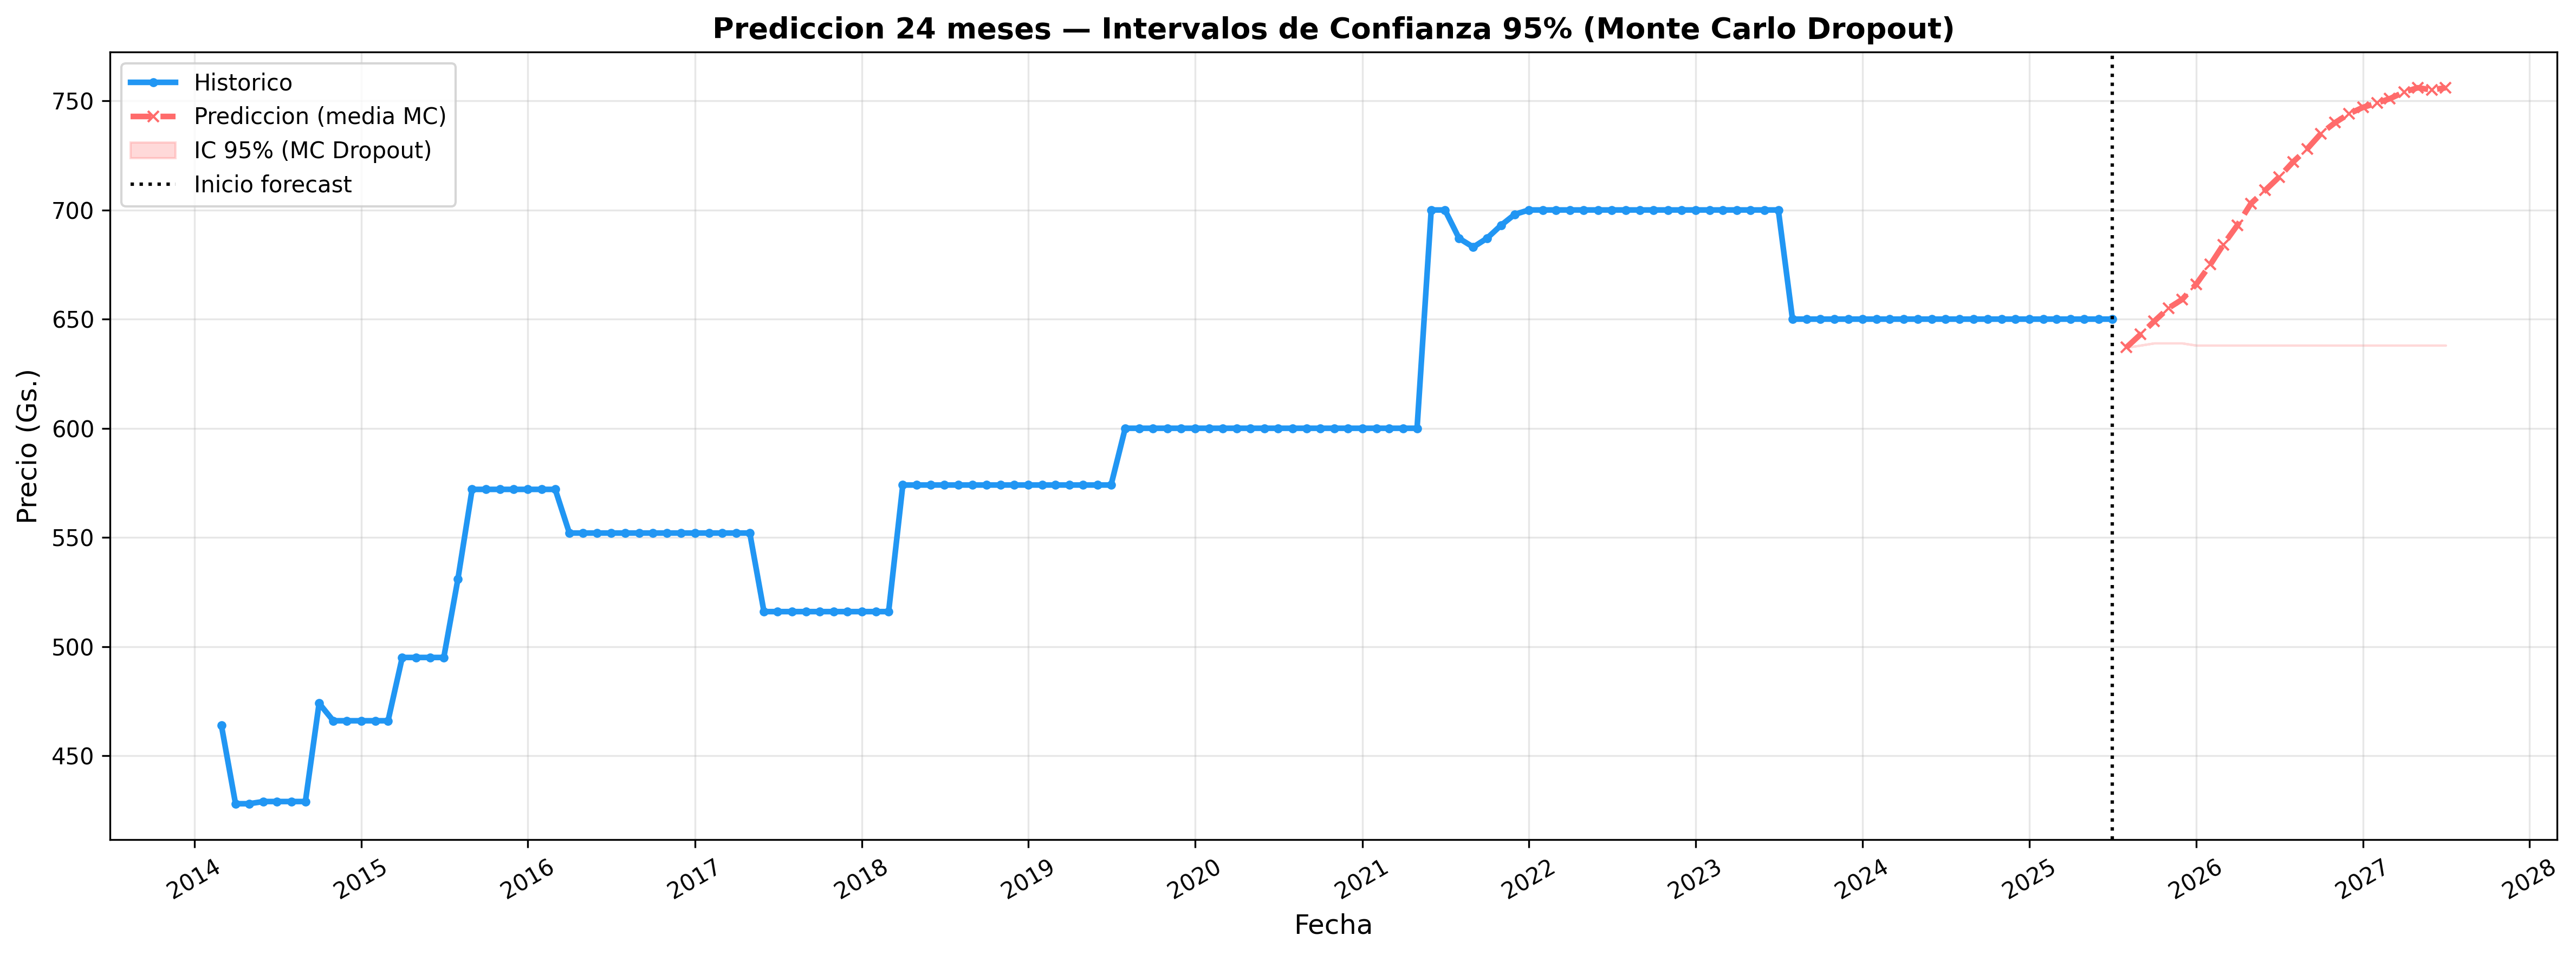
\includegraphics[width=\textwidth]{predicciones/prediccion_ladrillo_lstm/resultados_con_covid/forecast_ic_monte_carlo.png}
    \caption{IC Monte Carlo Dropout del pronóstico LSTM para ladrillo --- escenario con pandemia.}
    \label{fig:lstm_ladrillo_ic_mc_con_covid}
\end{figure}

\justify
Bajo el escenario con efecto pandémico, el rango de precios predicho se sitúa entre Gs.~637 y Gs.~756, con una dispersión considerablemente mayor que en el escenario sin pandemia. La comparación entre ambos escenarios muestra que el efecto pandémico eleva el precio máximo predicho del ladrillo de Gs.~644 a Gs.~756, un incremento del 17,4\,\% en el límite superior del rango. Este resultado indica que el modelo LSTM identifica un impacto alcista de las disrupciones pandémicas sobre el precio del ladrillo, aunque proporcionalmente menor que el efecto observado en el cemento (29,7\,\%). La menor magnitud puede atribuirse a que el ladrillo, como material de producción predominantemente local con cadenas de suministro más cortas, es menos sensible a las disrupciones logísticas internacionales.
